\documentclass[11pt]{report}
\usepackage[T1]{fontenc}
\usepackage{graphicx}
\usepackage{caption}
\usepackage{graphicx}
\usepackage{subcaption}
\usepackage[polish]{babel}
\usepackage[utf8]{inputenc}
\usepackage{lmodern}
\usepackage[pdftex]{graphicx}
\usepackage{alltt}
\usepackage{url}
\selectlanguage{polish}
\usepackage{amsmath}
\usepackage[top=3cm, bottom=3cm, left=3cm, right=3cm]{geometry}
\usepackage[chapter]{algorithm}
\usepackage{algorithmic}

\title{System do automatyzacji procesu składania planu zajęć z wykorzystaniem algorytmów genetycznych}
\author{
	Katarzyna Śmietanka \\
	Filip Czajkowski \\
	Tomasz Dziopa\\
	Paweł Jastrzębski
}
\begin{document}

%
% przeczytaj: http://en.wikibooks.org/wiki/LaTeX/Document_Structure
%

\maketitle
\tableofcontents


\chapter{Wstęp}

\section{Kontekst zagadnienia}
\textit{Katarzyna Śmietanka}
\par Problem układania planu zajęć dotyczy wielu instytucji głównie związanych ze szkolnictwem, od szkoły podstawowej aż do szkół wyższych. Zadanie sprowadza się do przygotowania graficznego rozkładu zajęć: dla poszczególnych klas - uczniów uczęszczających do danej klasy, planu zajęć dla każdego z uczących nauczycieli oraz rozkładu zajęć odbywających się w poszczególnych salach. Układanie planów zajęć nawet dla niewielkiej szkoły wymaga dużego wysiłku oraz nakładu czasowego. Problem staje jeszcze bardziej skomplikowany dla szkół ponadgimnazjalnych, do których uczęszcza więcej uczniów a tym samym jest więcej klas, nauczycieli oraz realizowanych przedmiotów. Ponadto, istnieje wiele wariantów tego problemu; na niektórych uczelniach, gdzie studenci sami mogą wybierać zajęcia, złożoność problemu jest o wiele większa. Trudność problemu związana jest z podstawowymi kryteriami, które musi spełniać plan zajęć aby był właściwy: dwa różne zajęcia, na które zapisany jest minimum jeden student nie mogą się odbywać w tym samym czasie, dwa różne zajęcia w tym samym czasie nie mogą odbywać się w tej samej sali oraz nauczyciel w danym momencie może nauczać tylko jednego przedmiotu. Rozszerzeń tych ograniczeń jest wiele, a uwzględnienie każdego z nich, często konieczne do stworzenia realnego planu zajęć jest niezbędne. Wprowadzanie kolejnych ograniczeń znacznie utrudnia problem, który i tak jest stosunkowo skomplikowany.
\par Pomysł tematu pracy inżynierskiej wyniknął z przyglądania się na przestrzeni naszej edukacji planom zajęć, które często odbiegały od idealnego według naszej opinii. Plan zajęć często zawierał sporo przerw między obowiązkowymi zajęciami, zajęcia zaczynały się bardzo wcześnie lub kończyły bardzo późno, co w znacznym stopniu utrudniało powrót do domu bądź też dopasowanie innych pozauczelnianych zajęć do naszego planu.
\par Problem ułożenia planu zajęć podejmowany był w wielu pracach naukowych również na Politechnice Gdańskiej, co świadczy o tym że ułożenie bezkonfliktowego planu zajęć jest problemem stosunkowo trudnym do rozwiązania a zarazem bardzo ciekawym, ponieważ w bezpośredni sposób dotyczy każdej uczącej się osoby. Dlatego też na przestrzeni wielu lat powstało wiele różnych podejść do tego problemu od algorytmów klasycznych poprzez różnego typu algorytmy sztucznej inteligencji.
\par Problem układania graficznych rozkładów nie tylko związany jest ze szkolnictwem, ale również dotyczy układania rozkładów jazdy komunikacji miejskiej \cite{com}, planu zajęć dla pracowników \cite{worker} oraz terminarza zawodów sportowych \cite{sport}.
\section{Cel}
\par Celem naszej pracy jest stworzenie systemu do automatyzacji procesu układania planów zajęć z wykorzystaniem Algorytmu Genetycznego (Genetic Algorithm).  W przeciągu ostatnich lat pojawiły się nowe podejścia, algotymy rozwiązujące problem układania planu zajęć, które postawiły algorytm genetyczny w nowym świetle. Chęć głębszego zapoznania się z postawionym przed nami problemem sprawiła, że zdecydowaliśmy się na rozszerzenie zagadnienia tematu naszej pracy inżynierskiej o kolejne implementacje algorytmów: Algorytm Roju Cząsteczek (Particle Swarm Optimization) oraz Algorytm Adaptacyjny Tabu (Adaptive Tabu Search). Ponadto w celu urzeczywistnienia problemu zdecydowaliśmy się na przystosowanie działania naszych algorytmów do realych danych, uzyskanych z jednej z gdyńskich szkół ponadgimnazjalnych.
\par Implementacja algorytmów: Genetycznego, Roju Cząsteczek oraz Adaptacyjnego Tabu postawiła nas przed ciekawą możliwością porównania działania tych algorytmów, co jak się okazuje nie jest łatwym zadaniem.
\section{Zakres pracy}
\par Na realizację postawionego celu składa się:
\begin{enumerate}
\item System do automatyzacji procesu układania planu zajęć
\begin{enumerate}
\item Frontend — aplikacja kliencka, odpowiadająca za interakcję z użytkownikiem: wprowadzanie danych wejściowych, wybór algorytmu do generowania planu zajęć oraz wizualizacja wygenerowanego planu zajęc w Ext JS Calendar.
\item Backend - generowanie planu zajęć z danych prowadzonych przez użytkownika 
\end{enumerate}
\item Implementacja algorytmów
\begin{enumerate}
\item Algorytm Genetyczny
\item Algorytm Roju Cząsteczek
\item Algorytm Adaptacyjny Tabu
\end{enumerate}
\item Przetworzenie danych szkolnych do zaimplementowanych algorytmów
\item Porównanie działania algorytmów

\end{enumerate}


\section{Podział zadań i obowiązków}
\begin{enumerate}
\item Tomasz Dziopa 
\begin{itemize}
\item Implementacja Algorytmu Adaptacyjnego Tabu
\item Przystosowanie działania algorytmu (ATS) do danych szkolnych
\item Implementacja systemu do automatyzacji procesu układania planów zajęć: stworzenie interfejsu użytkownika, wizualizacja wygenerowanych planów w Ext JS Calendar
\end{itemize}
\item Paweł Jastrzębski
\begin{itemize}
\item Implementacja Algorytmu Roju Cząsteczek
\item Implementacja systemu do automatyzacji procesu układania planów zajęć: stworzenie formularza do dodawania zadań, list do wyświetlania zadań, zdalne uruchamianie zadań poprzez rozproszoną kolejkę 
\end{itemize}
\item Filip Czajkowski
\begin{itemize}
\item Implementacja Algorytmu Genetycznego
\item Przystosowanie działania algorytmu (GA) do danych szkolnych
\item Przygotowanie dokumentacji dla Systemu do automatyzacji procesu układania planów zajęć
\end{itemize}
\item Katarzyna Śmietanka
\begin{itemize}
\item Implementacja Algorytmu Adaptacyjnego
\item Przystosowanie działania algorytmu (ATS) do danych szkolnych
\item Przetworzenie danych szkolnych do struktury zaimplementowanych algorytmów
\item Porównanie działania algorytmów, przygotowanie wizualizacji danych wejściowych
\end{itemize}
\end{enumerate}
\section{Środowisko pracy i narzędzia}
\paragraph{} Przy tworzeniu pracy inżynierskiej korzystaliśmy z repozytorium git w serwisie github.com \cite{github} z podpiętym narzędziem typu \textit{continuous integration} o nazwie travis \cite{travis}. Praktycznie cały kod został napisany w języku Python w wersji interpretera 2.7.6. Do testów jednostkowych użyto modułu \verb#nosetests#, aplikacja webowa została oparta o framework \verb#django# w wersji 1.6 i rozproszoną kolejkę zadań \verb#celery# \cite{celery}.
\paragraph{} 

<<<<<<< HEAD

\chapter{Opis problemu układania planu zajęć}
\textit{Tomasz Dziopa}
\paragraph{}Układanie planu zajęć można sformułować jako problem przydzielenia zdarzeń do przedziałów czasowych i zasobów, w taki sposób, żeby nie naruszyć odpowiednio skonstruowanych ograniczeń. Ograniczenia można podzielić na:
\begin{itemize}
\item ,,twarde'' - naruszenie ich powoduje, że utworzony plan zajęć jest niepoprawny,
\item ,,miękkie'' - naruszenia ich wyznaczają jakość utworzonego poprawnego planu zajęć. Im więcej naruszeń, tym jakość planu jest niższa.
\end{itemize}
\paragraph{}W przypadku problemu układania planu zajęć na uczelni problem możemy sprowadzić do następującej postaci:
\begin{itemize}
\item zdarzeniami będą powtarzające się zajęcia - wykłady, laboratoria, lekcje
\item zasobami będą sale, w których są prowadzone zajęcia i wykładowcy
\item ograniczenia twarde najczęściej uwzględniają:
	\begin{itemize}
	\item zajęcia dla jednej klasy nie mogą odbywać się w tym samym czasie,
	\item wykładowca nie może prowadzić równocześnie dwóch różnych zajęć,
	\item w jednej sali mogą odbywać się tylko jedne zajęcia,
	\item niektóre zajęcia muszą odbywać się w sali przystosowanej do specyfiki zajęć 
	\end{itemize}
\item ograniczenia miękkie definiuje się odrębnie dla placówek zależnie od ich priorytetów
\end{itemize}



%Problem układania planu zajęć jest niezwykle ważnym problemem. Jest obecny w wielu dziedzinach, gdyż przy niewielkich modyfikacjach można przenieść go na problem ustalania rozkładów jazdy, czy planowania grafiku pracowników, gdzie znalezienie lepszego rozwiązania prowadzi do oszczędności czasu i zasobów. 
\section{Klasyfikacja problemu}
\subsection{Problem NP-zupełny}
\paragraph{}Problem układania planu zajęć jest klasyfikowany jako NP-zupełny, co można w łatwy sposób udowodnić poprzez redukcję problemu k-kolorowania wierzchołkowego grafu $G(V, E)$, gdzie $V$ zawiera zdarzenia, a $E$ konflikty między nimi, do decyzyjnej wersji problemu układania planu zajęć (czy da się skonstruować plan zajęć obejmujący $k$ przedziałów czasowych) 
\paragraph{}Problem k-kolorowania wierzchołkowego to problem decyzyjny, który polega na odpowiedzi na pytanie, czy dany graf da się pokolorować wierzchołkowo na dokładnie $k$ kolorów. Przypomnijmy, że w każdym poprawnym pokolorowaniu każde dwa wierzchołki połączone ze sobą krawędzią muszą mieć przyporządkowane różne kolory. W grafie $G(V,E)$ krawędziami połączone są zdarzenia, które nie mogą odbywać się w tym samym czasie. Jeżeli przyjmiemy, że kolorom w pokolorowaniu odpowiadają poszczególne przedziały czasowe otrzymujemy redukcję w czasie wielomianowym ze względu na liczbę wierzchołków i krawędzi do problemu k-kolorowania wierzchołkowego grafu. Bardziej formalny dowód na tą redukcję, jak i inne redukcje z innych problemów NP-zupełnych zawiera \cite{npcomplete}.


\section{Przegląd algorytmów}
\subsection{Metaheurystyki}
\paragraph{}Problem układania planu zajęć jest NP-zupełny, więc nie istnieje deterministyczny algorytm, który zwracałby dokładny wynik w czasie wielomianowym. Konieczne jest więc zastosowanie \textbf{metaheurystyk} - niedeterministycznych algorytmów, które wspomagają przeszukiwanie przestrzeni rozwiązań, w celu znalezienia najlepszego rozwiązania. Metaheurystyki często bazują na obserwacjach różnych procesów zachodzących w naturze. Znane są zastosowania różnego rodzaju metaheurystyk do rozwiązania naszego problemu.
\subsubsection{Algorytm genetyczny}
\paragraph{} Być może najbardziej popularne i uniwersalne rozwiązanie. Proces optymalizacji rozwiązania odwzorowuje sposób ewolucji genetycznej osobników przystosowujących się do środowiska, w którym przebywają. Swoje odwzorowanie mają zatem metody selekcji lepiej przystosowanych osobników, którzy dożyją następnego pokolenia, operacja krzyżowania osobników w celu stworzenia potomstwa czy też mutacja wprowadzająca drobne zmiany w materiale genetycznym. Algorytm iteracyjne polepsza swoje rozwiązanie coraz dokładniej przeszukując przestrzeń możliwych rozwiązań. Czynnik losowy odgrywa dużą rolę w wymienionych wcześniej procesach, co nie gwarantuje bardzo skutecznych rezultatów.
\subsubsection{Algorytm wyszukiwania harmonicznego}
Jedno z najnowszych rozwiązań (powstałe w 2001 roku). Naśladuje proces poszukiwania harmonii przez grających razem muzyków, której jakość jest miarą rozwiązania. Przechowując w pamięci najlepsze dotychczasowe współbrzmienia oraz tworząc nowe (losowe) wysokości odgrywanych dźwięków, muzycy poprawiają wzajemną harmonię. Rozwiązanie to początkowo zebrało wiele pozytywnych recenzji i zakładano, że może wnieść wiele skutecznych rozwiązań w dziedzinie problemów optymalizacyjnych, lecz nadzieje te zostały porzucone ze względu na duże podobieństwa do pozostałych algorytmów ewolucyjnych.
\subsubsection{Algorytm optymalizacji rojem cząsteczek}
Metoda ta stara się naśladować zachowania występujące w przyrodzie. Jest to technika ewolucyjna wzorowana na sposobie poruszania się i inteligencji roju owadów poszukującego optymalnego miejsca do pożywienia się. Dokładniejszy opis algorytmu znajduje się w punkcie 4.2.

\subsubsection{Algorytm symulowanego wyżarzania}
\paragraph{} Metoda przeszukiwania iteracyjnego zainspirowana procesem wyżarzania w przemyśle metalowym. Przechowujemy specjalną zmienną, która symuluje malejącą ,,temperaturę'' otoczenia. W każdej iteracji przeglądamy sąsiadów i z prawdopodobieństwem proporcjonalnym do ,,temperatury'' akceptujemy rozwiązanie gorsze od aktualnego.


\subsubsection{Algorytm Tabu Search}
\paragraph{} Metoda iteracyjnego przeszukiwania najlepszego rozwiązania, która bazuje na liście tabu - liście ruchów zabronionych, których nie można wykonać przez określoną liczbę iteracji. Dokładny opis algorytmu znajduje się w punkcie 4.1.3.

\subsection{Hiperheurystyki}
\paragraph{}Nieco innym podejściem do rozwiązania problemu układania planu zajęć jest zastosowanie hiperheurystyki. \textbf{Hiperheurystyka} to algorytm, który ma za zadanie odnalezienie najlepszej metaheurystyki mającej na celu znaleźć optymalne rozwiązanie. Przykładem hiperheurystyki może być algorytm Adaptive Tabu Search, opisany szerzej w punkcie 4.1, gdzie metaheurystykami niskiego poziomu są procedury Tabu Search dla dwóch struktur sąsiedztwa, a metaheurystyką jest iteracyjne przeszukiwanie lokalne, które steruje głębokością procedury Tabu Search i wprowadza operator zaburzeń rozwiązania.
\paragraph{}Innym przykładem hiperheurystyki jest algorytm opisany w \cite{gbhh}. Autorzy jako metaheurystyki niskiego poziomu wybrali 5 różnych kolejności, w których można rozpatrywać wierzchołki grafu kursów i konfliktów między nimi. Metaheurystyka wysokiego poziomu - w tym przypadku Tabu Search, gdzie lista Tabu przechowuje kombinacje dwuelementowe metaheurystyk niskiego poziomu - wybiera dwie metaheurystyki, które nie występują na liście Tabu, przyporządkowywuje według nich kolejne kursy i porównuje wynik z najlepszym.

\subsection{Algorytmy \textit{state-of-the-art}}

\paragraph{} Inną grupą algorytmów, na które można się natknąć w literaturze są algorytmy tzw. \textit{state-of-the-art} - wielofazowe algorytmy, które kolejnych fazach wykonują po kilka różnych metaheurystyk. Przykładem takiego algorytmu jest algorytm, który wygrał konkurs ITC w 2003 roku, opisany w \cite{kostuch}.


\section{Przegląd powstałych systemów}



\subsection{aSc TimeTables}
Rozbudowane komercyjne narzędzie, które umożliwia automatyczne wygenerowanie planu zajęć na podstawie zebranych wymagań. Posiada bardzo zaawansowane możliwości edycji wygenerowania planu, wprowadzania zastępstw nauczycieli i wizualizacji. Możliwości sterowania generowaniem są ograniczone - można ustalić czas generowania (krótki - długi - bardzo długi) i stopień spełniania warunków. Program jest adresowany do dyrektorów i osób zarządzających planami lekcji, jego obsługa jest bardzo prosta. Wadą jest scentralizowane wprowadzanie ograniczeń, nieestetyczny interfejs i cena 
(od 499 USD za wersję podstawową, do 3995 USD za wersję z rozszerzonym wsparciem i generowaniem planów dla poszczególnych uczniów)
\begin{figure}[H]
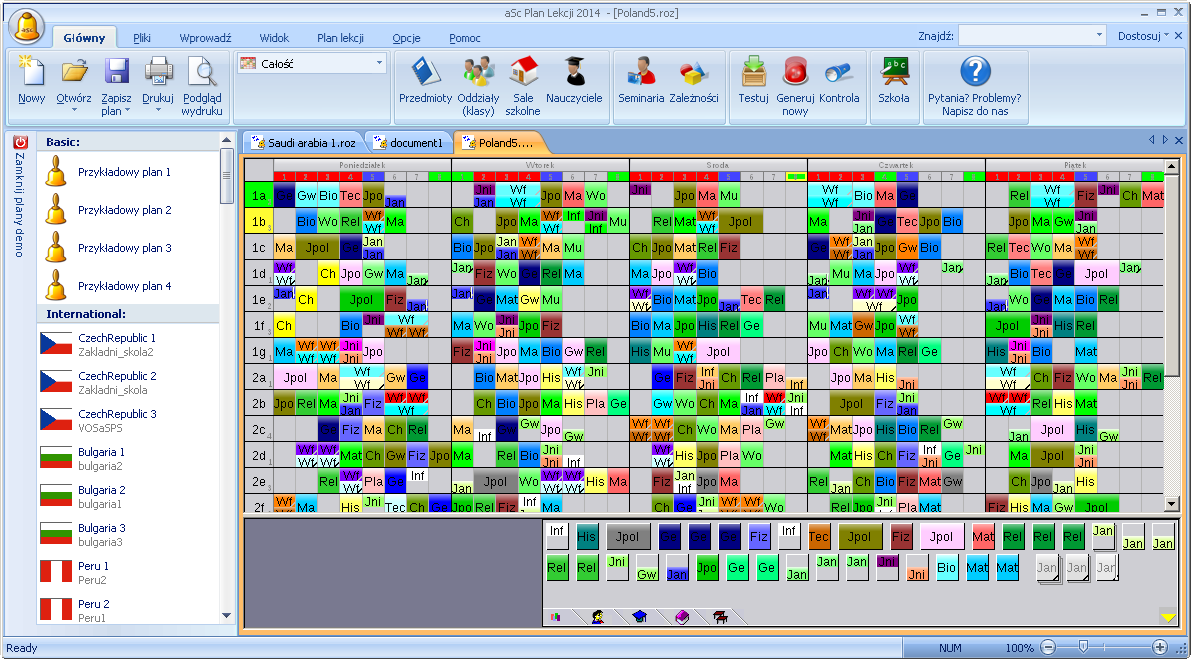
\includegraphics[width=15cm]{img/asc2.png}
\caption{Zrzut ekranu z programu aSc. Przy przenoszeniu zajęć konfliktujące okresy podświetlają się na czerwono}
\end{figure}

\subsection{Mimosa}
Komercyjny program, który umożliwia wprowadzanie ograniczeń, automatyczne generowanie planu zajęć i optymalizowanie już istniejącego planu. Interfejs aplikacji jest nieczytelny i chaotyczny, cały program sprawia wrażenie przestarzałego. Nie można sterować procesem generowania, który jest realizowany w bardzo szybki sposób, jednak dla przykładowych danych nie przydziela wszystkich zajęć, pomimo tego, że jest to możliwe. Aplikacja jest uniwersalna, można dostosowywać problem do własnych potrzeb, jednak bez uprzedniego przeszkolenia jest to bardzo trudne. Najtańsza licencja na jedno stanowisko kosztuje 500 euro.
\begin{figure}[H]
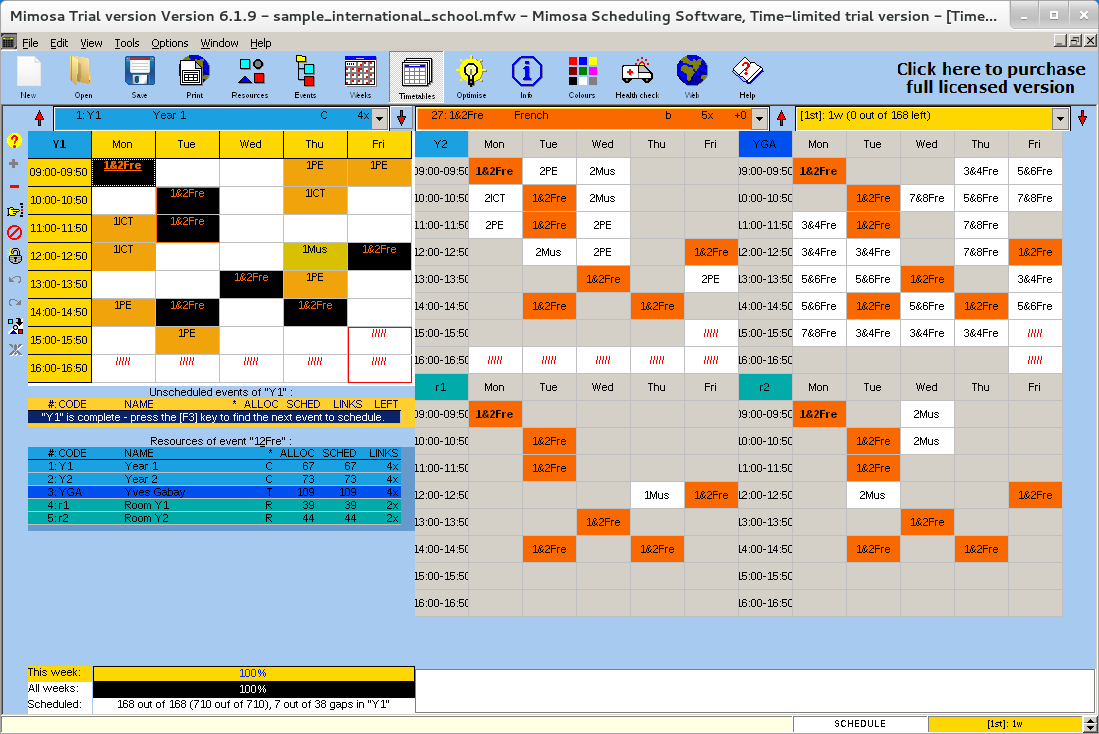
\includegraphics[width=15cm]{img/mimosa.png}
\caption{Zrzut ekranu z widoku planu zajęć programu Mimosa}
\end{figure}
\subsection{FET - Free Evolutionary Timetable}
Jest to program darmowy, stworzony dla platformy Linux, rozpowszechniany na zasadach licencji GNU GPL. Napisany w C++ z wykorzystaniem biblioteki Qt, dane pobiera z plików w formacie XML. W swojej początkowej formie opierał się na algorytmie genetycznym, który jednak poczynając od wersji 5.0.0 wydanej w 2007 roku został zastąpiony autorską heurystyką nazwaną przez autora \emph{rekursywnym zamienianiem}. Naśladuje on proces manualnego układania planu zajęć i okazał się dużo szybszy i wydajniejszy dla złożonych problem w porównaniu ze swoim poprzednikiem. Jego rozbudowany interfejs umożliwia śledzenie procesu ewolucji najlepszego rozwiązania.
\subsection{Tablix}
Jest to polski produkt typu \emph{open source}, jego autorem jest Tomasz Solc. Program powstał w technologii języka C z użyciem pakietu PVM, który umożliwia zrównoleglenie obliczeń, co znacząco przyspiesza działanie algorytmu. Dane wejściowe muszą znajdować się w plikach XML. Głównym mechanizmem, na którym opiera się program jest zrównoleglony algorytm genetyczny. Zastosowania stworzonego jądra systemu mogą dotyczyć najróżniejszych problemów optymalizacyjnych, lecz w swojej pierwotnej implementacji zostało przystosowane do problemu układania planu zajęć. Nie posiada natomiast interfejsu graficznego, który umożliwiałby edycję danych lub wizualizację wyników.


\chapter{Specyfikacja problemu}
\textit{Filip Czajkowski, Katarzyna Śmietanka} \\
\paragraph{}Specyfikacja problemu układania planu zajęć różni się bardzo w kontekście konkretnego przypadku. Dlatego też chcieliśmy, aby nasze implementacje opierały się na dobrze opisanym przypadku, który umożliwi jasne określenie wymagań względem naszych rozwiązań i pozwoli na ich jednoznaczne porównanie. Okazało się, że odbywający się co kilka lat międzynarodowy konkurs na najlepsze rozwiązanie w tej dziedzinie bardzo dobrze spełnia te założenia.
\section{International Timetabling Competition 2007}
\textit{Filip Czajkowski} \\
\subsection{Opis konkursu}
\paragraph{International Timetabling Competition (ITC)}\cite{itc} to międzynarodowy konkurs w dziedzinie układania planów zajęć organizowany przez międzynarodowe środowisko akademickie. Jego celem jest lepsze poznanie problemu rozkładania zajęć lub egzaminów na uczelni, z którym zmagają się od bardzo dawna i wciąż potrzebują stosowania lepszych rozwiązań. W 2007 roku odbyła się jego druga edycja, w której można było startować w dowolnej z trzech kategorii: 
\begin{itemize}
\item Układanie rozkładu sesji egzaminacyjnej na uczelni. W tym przypadku zakłada się, że wszyscy studenci zapisani na swoje zajęcia muszą mieć możliwość wzięcia udziału we wszystkich dotyczących ich egzaminach. Plan powstaje zatem po zapisaniu się wszystkich studentów na wybrane przez siebie przedmioty.
\item Tworzenie planu zajęć dla studentów zapisanych na konkretne zajęcia. W tym przypadku rozkład wszystkich zajęć obowiązujących przez cały semestr jest generowany w momencie, gdy studenci wybrali już przedmioty, na które zajęcia chcą uczęszczać. Ten model rozwiązania jest dostosowany do elastycznych programów nauczania, które uczelnie coraz częściej stosują.
\item Układanie planu zajęć dla każdego planu nauczania. Tworzony jest tygodniowy rozkład lekcji, które są przyporządkowane do poszczególnych programów nauczania, a także muszą spełniać ograniczenia czasowe narzucone przez władze uczelni. Udostępnione przykładowe dane przedmiotów, sal oraz wykładowców pochodzą z Uniwersytetu Udine we Włoszech.
\end{itemize}
W przewidzianym przedziale czasowym można było nadsyłać rozwiązania, które można było testować na części udostępnionych zestawach danych. Niedozwolone było stosowanie zrównoleglenia obliczeń w stosowanych rozwiązaniach. Ostatecznie, zwycięzcy w każdej z kategorii zostali ogłoszeni podczas konferencji w Montrealu w 2008 roku i każdy z nich otrzymał nagrodę pieniężną w wysokości 500\pounds .
\subsection{Konkurs a praca inżynierska}
\par Poszukując informacji o implementowanych przez nas algorytmach optymalizacyjnych w kontekście układania planu zajęć, natknęliśmy się na informacje o konkursie ITC w 2007 roku. Wspólnie stwierdziliśmy, że skorzystanie ze zdefiniowanych w nim ograniczeń i wymagań względem generowanego planu a także określona funkcja oceny rozwiązania bardzo pomoże nam zaprojektować nasze algorytmy oraz jednoznacznie je porównać. Nasze implementacje były tworzone pod kątem trzeciej kategorii konkursu, czyli rozkładu zajęć przedmiotów zawierających się we wcześniej zdefiniowanych programach nauczania.
\section{Sformułowanie problemu}

Celem jest stworzenie tygodniowego harmonogramu wykładów dla kilku kursów, z określoną liczbą dostępnych sal i przedziałów czasowych, w których mogą odbywać się zajęcia. Każdy wykład będący w programie danego kursu musi być przypisany do określonego przedziału czasu i sali tak by spełniał wejściowe ograniczenia. 
\subsection{Jednostki problemu}
\begin{itemize}
\item{\textbf{Dni, przedziały, okresy} - dzień podzielony jest na określoną liczbę przedziałów czasowych, okres para złożona z dnia i przedziału czasowego.}
\item{\textbf{Kursy i wykładowcy} - każdy kurs składa się z określonej liczby zajęć, które muszą być rozłożone w różnym czasie, na które uczęszcza określona liczna studentów i prowadzone są one przez konkretnego wykładowcę. Dla każdego kursu określona jest minimalna liczba dni, na które powinny być rozłożone zajęcia oraz okresy w których dane wykłady (zajęcia) nie mogą się odbywać.}
\item{\textbf{Sale wykładowe} - sale wykładowe mają ograniczoną liczbę dostępnych miejsc w pomieszczeniu.}
\item{\textbf{Program nauczania} - składa się z kilku kursów, na które uczęszcza grupa studentów.}
\end{itemize}
\subsection{Ograniczenia}
\subsubsection{Ograniczenia twarde}
Plan jest wykonywalny - czyli możliwy do realizacji, jeżeli żadne z wymienionych poniżej ograniczeń nie jest naruszone.
\begin{itemize}
\item  ${H_{1}}$ \textbf{Wykłady} - każdy kurs wchodzący w skład programu nauczania musi być przypisany do różnego okresu.
\item  ${H_{2}}$ \textbf{Zajętość sali} - żadne dwa wykłady nie mogą odbywać się w tym samym okresie w jednym pomieszczeniu.
\item  ${H_{3}}$ \textbf{Konflikty pomiędzy kursami} - zajęcia z tego samego programu nauczania bądź nauczanie przez tego samego wykładowcę muszą odbywać się w różnym czasie.
\item  ${H_{4}}$ \textbf{Dostępność wykładowcy} - zajęcia nie mogą się odbywać w czasie, w którym dany wykładowca nie może prowadzić zajęć.
\item ${H_{5}}$ \textbf{Typ sali} - każde z zajęć powinno odbywać się w odpowiedniej sali przystosowanej do przeprowadzania zajęć (odpowiednim typie sali) [*] - ograniczenie to dotyczy tylko $Szkolne\ dane\ wejściowe$
\end{itemize}
\subsubsection{Ograniczenia miękkie}
Ograniczenia te w bezpośredni sposób nie wpływają na wykonywalność planu zajęć, ale na jakość wygenerowanego planu zajęć, określoną na podstawie funkcji oceny.
\begin{itemize}
\item  ${S_{1}}$ \textbf{Wielkość sali} - liczba studentów uczęszczających na zajęcia w danej sali musi być mniejsza bądź równa liczbie dostępnych miejsc.
\item  ${S_{2}}$ \textbf{Stabilność pomieszczenia} - zajęcia wchodzące w skład jednego kursu powinny odbywać się w jednej tej samej sali, jeżeli jest to niemożliwe liczba sal w których odbywają się te zajęcia powinna być jak najmniejsza.
\item  ${S_{3}}$ \textbf{Minimalna liczba dni} - minimalna liczba dni na które powinny być rozłożone zajęcia z danego kursu.
\item  ${S_{4}}$ \textbf{Zwartość zajęć} - zajęcia wchodzące w skład jednego programu nauczania powinny odbywać się w jak najmniejszych odstępach czasowych między sobą. [*] - dotyczy to tylko $Danych\ konkursowych$
\end{itemize}
\subsection{Funkcja oceny - dla danych konkursowych}
\label{funkcjaOceny}
\textbf{Ograniczenia twarde} - podczas oceny końcowej wygenerowanego planu zajęć zliczane są poszczególne naruszenia ograniczeń twardych:\\
\begin{enumerate}
\item \textbf{Zajęcia / Wykłady} - naruszenie występuje w przypadku gdy zajęcia nie są przypisane do planu zajęć
\item \textbf{Zajętość sali} - naruszenie występuje gdy zostaną przypisane więcej niż jedne zajęcia do sali w tym samym czasie
\item \textbf{Konflikty} - naruszenie wystąpi wtedy, gdy dwa zajęcia będące w konflikcie odbywają się w tym samym czasie (tzn. ci sami studenci uczęszczają na te zajęcia lub prowadzone są przez tego samego wykładowcę)
\item \textbf{Dostępność} - naruszenie występuje gdy zajęcia odbywają się w czasie, w którym niedostępny jest wykładowca 
\end{enumerate} 

\textbf{Ograniczenia miękkie} - zliczanie punktów kary
\begin{enumerate}
\item \textbf{Wielkość sali} - Jeżeli liczba studentów jest większa niż liczba dostępnych miejsc w sali to za każdego dodatkowego studenta punkt kary pomnożony przez współczynnik ${a_{1} = 1}$ 
\item \textbf{Minimalna liczba dni}
Jeżeli liczba dni podczas których odbywają się zajęcia jest mniejsza niż minimalna liczba dni, podczas których powinny odbywać się zajęcia to do kary doliczamy różnicę między minimalną liczbą dni a liczbą dni, w których zajęcia się odbywają pomnożoną o współczynnik $a_{2} = 5$ 
\item \textbf{Zwartość zajęć}
Za każde zajęcia w planie, które nie przylegają do żadnych innych zajęć z tego samego programu nauczania, punkt kary pomnożony o współczynnik ${a_{3} = 2}$
\item \textbf{Stabilność pomieszczenia}
Te same zajęcia powinny odbywać się w jak najmniejszej liczbie różnych pomieszczań, za każde nowe pomieszczenie punkt kary pomnożony o współczynnik ${a_{4} = 1}$
\end{enumerate}

\subsection{Matematyczny zapis przestrzeni rozwiązań} \cite{tabu}
\par Na problem składa się ${n}$ kursów ${C = \{c_{1}, c_{2},...,c_{n}\}}$ które powinny być przydzielone do ${p}$ różnych okresów ${T = \{t_{1}, t_{2},...,t_{p}\}}$ oraz ${m}$ pomieszczeń w których mogą odbywać się zajęcia ${R = \{r_{1}, r_{2},...,r_{m}\}}$. Okres jest to para składająca się z dnia i przedziału czasowego (${d}$ - liczba dni a ${h}$ - liczba dziennych przedziałów czasowych, czyli ${p = d * h}$). Każdy z kursów składa się z ${n}$ zajęć ${L = \{l_{1},l_{2},...,l_{n}\}}$. Kursy wchodzą w skład ${s}$ programów nauczania ${CR = \{cr_{1}, cr_{2}, ..., cr_{s}\}}$, na program nauczania składają się kursy, na które uczęszczają ci sami studenci. 

\section{Dane wejściowe}
\label{sec:input_format}
\subsection{Konkursowe dane wejściowe}
\par Dane wejściowe zostały uzyskane z konkursu International Timetabling Competition 2007
\par Dane wejściowe są plikami tekstowymi, w których zawarte są ogólne informacje takie jak: liczba kursów, liczba dostępnych pomieszczeń, liczba dni na które mają być rozłożone zajęcia, liczba programów nauczania oraz ograniczenia precyzujące w jakich terminach nie mogą odbywać się zajęcia z danego kursu. Kolejno sprecyzowane są kursy, pomieszczenia, programy nauczania oraz ograniczenia w zadanym poniżej formacie:
\begin{verbatim}
Kursy: <Id Kurs> <Nauczyciel> <Liczba zajęć> <Minimalna liczba dni> <liczba studentów>
Sale: <Id Sala> <Pojemność sali>
Program nauczania: <Id Program Nauczania> <Liczba Kursów> <Ids Kursy>
Ograniczenia: <Id Kurs> <Dzień> <Okres>
\end{verbatim}
\begin{enumerate}
\item Każdy z kursów z danych wejściowych zawiera unikalny identyfikator, liczbę zajęć, która musi się odbyć w ramach tego kursu, minimalną liczbę dni oraz liczbę studentów, którzy uczęszczają na te zajęcia. 
\item Sale zawierają unikalny identyfikator oraz informację o maksymalnej liczbie studentów, która się zmieści w sali.
\item Na program nauczania składa się określona liczba kursów, których identyfikatory zawarte są w opisie programu nauczania  \verb#<Ids Kursy>#

\item W ramach ograniczeń umieszczona jest informacja o kursie \verb#<Id Kurs>#
 który nie może odbyć się w danym dniu w danym okresie.
\end{enumerate}
\subsection{Szkolne dane wejściowe}
\par Dane z roku szkolnego 2013/2014 uzyskane z jednej ze szkół gdyńskich ponadgimnazjalnych, która jest połączeniem szkoły zawodowej, technikum oraz liceum.
\par Dane zostały przystosowane do formatu ,,Konkursowych danych wejściowych'' rozszerzając je o pojęcie typu sali. Szczegółowy proces przetworzenia danych został opisany w sekcji ,,Etapy przetwarzania danych szkolnych''.
\begin{verbatim}
Kursy: <Id Kurs> <Nauczyciel> <Liczba zajęć> <Minimalna liczba dni> 
	   <liczba studentów><Typ sali>
Sale: <Id Sala> <Pojemność sali> <Typ sali>
Program nauczania: <Id Program Nauczania> <Liczba Kursów> <Ids Kursy>
Ograniczenia: <Id Kurs> <Dzień> <Okres>
\end{verbatim}
Rozszerzenie formatu danych wejściowych:
\begin{enumerate}
\item Wprowadzono \verb#<Typ sali>#, który przyjmuje poniżej zdefiniowane wartości:
\begin{verbatim}
n - zwykła sala lekcyjna
w - sala warsztatowa
l - biblioteka
o - poza szkołą
e - sala gimnastyczna / boisko szkolne / basen 
c - sala laboratoryjna (komputerowa)
\end{verbatim}
\item Został wprowadzony \verb#<Typ sali># dla każdego z kursów określający w jakich rodzajach sal mogą odbywać się zajęcia z tego kursu.
\end{enumerate}

\chapter{Projekt systemu}
\section{Cele systemu}
\paragraph{}Wytworzony system miał na celu umożliwić wygenerowanie rozkładu zajęć na podstawie dostępnych danych opisujących daną placówkę edukacyjną. Główny wysiłek został położony na implementację algorytmów, które plan układają, natomiast aplikacja webowa miała służyć jako prosty interfejs do ich wywoływania. Poprzez zastosowanie kilku algorytmów do rozwiązania tego problemu, system umożliwiać miał porównanie ich wydajności. Dodatkowo miał także udostępniać wizualną prezentację powstałego planu dla danego programu nauczania, aby móc go ocenić pod kątem praktycznego zastosowania.
\section{Wymagania}
\paragraph{}Powstały system miał narzucone następujące ograniczenia techniczne:
\begin{itemize}
\item Aplikacja po stronie klienta jest dostępna z poziomu przeglądarki z obsługą JavaScript i wymaga jedynie aktywnego połączenia z serwerem. Za stronę wizualną odpowiadać będą:
\begin{enumerate}
\item framework JavaScript \emph{ExtJS 4.2} z komponentem \emph{Ext JS Calendar}
\item style i widoki \emph{Bootstrap 3.0.3}.
\end{enumerate}
\item Aby uruchomić algorytmy po stronie serwera, potrzebne jest posiadanie zainstalowanych następujących komponentów:
\begin{enumerate}
\item kompilator języka \emph{Python 2.7}
\item środowisko wytwórcze aplikacji internetowych w języku Python \emph{Django 1.6}
\item system rozproszonego kolejkowania zadań \emph{Celery 3.1}
\item system komunikacji kolejek systemowych \emph{RabbitMQ 3}
\item obsługa bazy danych \emph{SQLite3}
\end{enumerate}
\end{itemize}
\paragraph{}Wymagania funkcjonalne:
\begin{itemize}
\item Konieczność logowania się w celu korzystania z systemu.
\item Wywołanie procesu generowania planu zajęć z możliwością wyboru algorytmu.
\item Możliwość ustawienia limitu czasowego na czas działania procesu.
\item Pobieranie z pliku tekstowego wedle ustalonego wzorca zestawu ograniczeń opisujących potrzeby rozkładu zajęć.
\item Podgląd listy wykonanych wcześniej zadań oraz stanu uruchomionych obecnie procesów.
\item Wybranie z listy zadań konkretnego przypadku i odczytanie informacji o przyporządkowanych zajęciach do poszczególnych kursów.
\item Pobranie wygenerowanego rozkładu zajęć w formie pliku \emph{.CSV}.
\item W widoku zakończonego zadania możliwość wybrania z listy programów nauczania dowolnego z nich i wizualizacji planu w komponencie kalendarza.
\end{itemize}
\section{Zastosowanie}
\paragraph{}Wytworzony system może mieć zastosowanie dwojga rodzaju. Pierwsze z nich należy do pola naukowo - badawczego i szczególnie pod tym kątem było projektowane. Dotyczy ono samego zagadnienia układania planu zajęć, umożliwia porównanie zastosowanych trzech metod pod kątem np. czasu pracy czy samej efektywności procesu. Drugim obszarem zastosowań jest platforma biznesowa, choć dość ograniczona w tym przypadku. Posiadając dane na temat jakiejś placówki dydaktycznej w odpowiednim formacie będziemy mogli ułożyć dla niej realny rozkład zajęć. Udostępniany przez system sposób wizualizacji wynikowego planu umożliwia poddanie go trafnej ocenie przydatności przez człowieka.
\subsection{Przypadki użycia}
\begin{itemize}
\item{\textbf{Aktorzy}} - Wszyscy mogą korzystać z systemu w ten sam sposób, więc istnieje jeden aktor, podstawowy użytkownik systemu. Natomiast aby przeprowadzić jakąkolwiek operację konieczne jest zalogowanie się na wcześniej utworzone konto.
\end{itemize}
\paragraph{}Przypadki użycia systemu, pod których kątem zostały zdefiniowane wymagania i wytworzony cały system prezentują się następująco.
\begin{center}
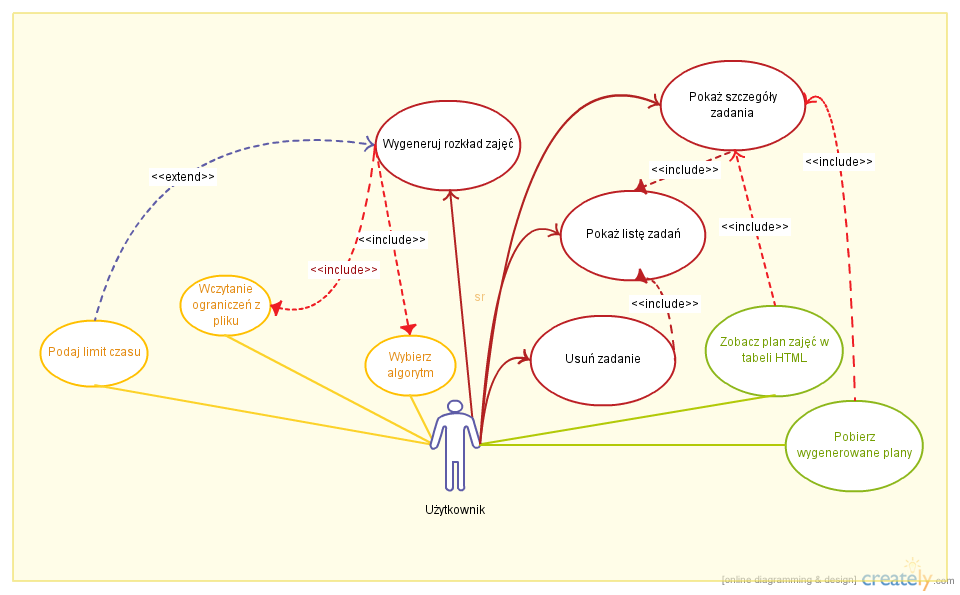
\includegraphics[width=0.8\textwidth]{img/InzynierkaUseCase.png}
\end{center}
\begin{enumerate}
\item \textbf{Wygeneruj rozkład zajęć} - Po zalogowaniu z górnego menu wybrać opcję \emph{Add task} i wyświetli się widok umożliwiający wyspecyfikowanie nowego zadania generującego rozkład zajęć.
\item \textbf{Podaj limit czasu} - Po wybraniu z menu opcji \emph{Add task} możliwe będzie wpisanie limitu na czas działania algorytmu w sekundach.
\item \textbf{Wczytanie ograniczeń z pliku} - Po wybraniu z menu opcji \emph{Add task} widoczny będzie formularz umożliwiający wybór pliku ze zdefiniowanym problemem.
\item \textbf{Wybierz algorytm} - Po wybraniu z menu opcji \emph{Add task} w widocznym formularzu dostępna jest lista trzech algorytmów, które będę sterować procesem generacji planu.
\item \textbf{Pokaż szczegóły zadania} - Po wybraniu zadania z listy poprzez kliknięcie \emph{Details} ukarze się widok ze szczegółami dotyczącymi konkretnego planu.
\item \textbf{Pokaż listę zadań} - Po wybraniu z menu opcji \emph{List all tasks} pokaże się lista dotychczas wykonanych zadań.
\item \textbf{Usuń zadanie} - Po wybraniu z menu opcji \emph{List all tasks} pokaże się lista zadań, a każde z nich będzie można usunąć poprzez kliknięcie na przycisk \emph{Delete}, co wywoła następnie odświeżenie listy.
\item \textbf{Zobacz plan zajęć w tabeli HTML} - Po wybraniu konkretnego zadania z widoku listy, dla każdego elementu z listy programów nauczania zawartych w planie, dostępny będzie przycisk wywołujący wizualizację wygenerowanego dla niego planu w postaci komponentu kalendarza.
\item{Pobierz wygenerowane plany} - Po wybraniu konkretnego zadania z widoku listy, dostępny będzie przycisk umożliwiający pobranie wszystkich planów w postaci arkuszy w pliku \emph{.csv}.
\end{enumerate}
\section{Architektura systemu}
\paragraph{} Ogólna architektura systemu oparta jest na modelu klient - serwer. Wszystkie operacje logiczne są wykonywane po stronie serwera, natomiast część kliencka odpowiada jedynie za pobranie danych i prezentację wyników. W części serwera zawarte są następujące komponenty.
\begin{enumerate}
\item Oprogramowanie obsługi serwera wykonane w środowisku \emph{Python}, które generuje widok strony internetowej, odbiera żądania klienta itd.
\item Moduł odpowiedzialny za wyświetlanie planów zajęć na podstawie informacji zawartych w pliku wynikowym algorytmu.
\item Baza danych \emph{SQLite} zawierająca informacje o użytkownikach systemu oraz wykonanych zadaniach.
\item Moduły generujące plany zajęć realizujące poszczególne algorytmy wykonane w technologii \emph{Python}.
\item Komponent \emph{Celery} realizujący zadania z kolejki zadań wywołujący wskazane algorytmy.
\end{enumerate}
\begin{figure}[H]
  \caption{Diagram komponentów systemu}
  \centering
    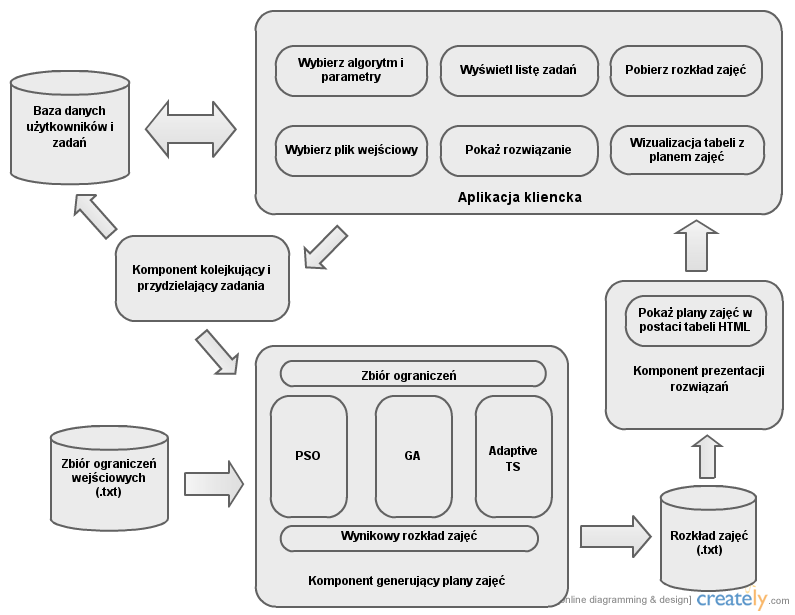
\includegraphics[width=0.8\textwidth]{img/ComponentsDiagram.png}
\end{figure}
\section{Rozwiązania implementacyjne}
\paragraph{Komunikacja} - schemat komunikacji w systemie po stronie serwera podczas wywołania zadania generującego plan prezentuje poniższy diagram.
\begin{figure}[H]
  \caption{Diagram komunikacji po stronie serwera}
  \centering
    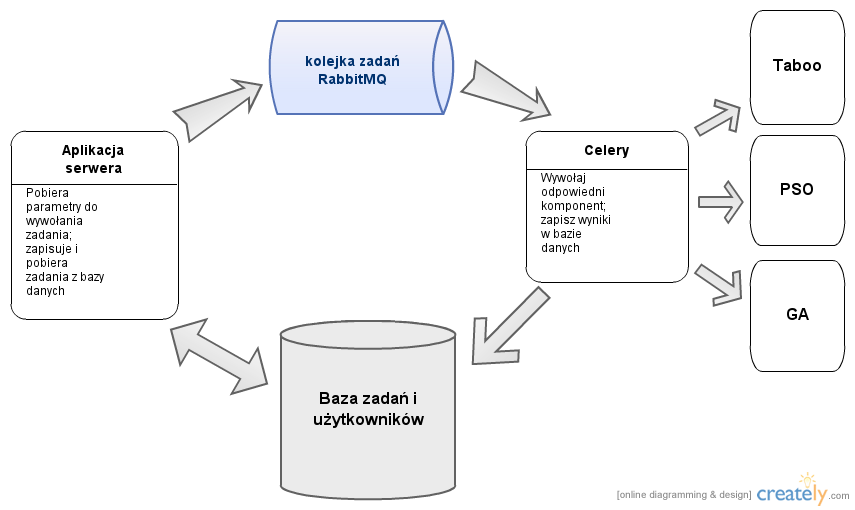
\includegraphics[width=0.8\textwidth]{img/SystemCommunication.png}
\end{figure}
Gdy użytkownik prześle plik wejściowy i parametry wykonania, następuje wywołanie procedury wytworzenia planu zajęć. Aplikacja serwera przekazuje wiadomość o potrzebie wykonania zadania wraz z informacją jaki algorytm wywołać i gdzie znajduje się plik wejściowy. Zlecone zadania są zapamiętywane w kolejce systemowej. Następnie, gdy obiekt wywołujący zadania jest wolny, podbiera z kolejki zadanie i następnie wywołuje odpowiedni komponent wskazany przez typ stosowanego algorytmu. Po wykonaniu zadania zapisuje zwrócony plan zajęć do pliku i dodaje w bazie danych wpis o kolejnym zakończonym zadaniu. Dzięki tej informacji aplikacja kliencka może później pobrać informacje o wygenerowanym planie.
\paragraph{}W celu zapisywania wygenerowanych planów, została stworzona  na serwerze określona struktura plików. Istnieją dwa foldery \emph{input} oraz \emph{output}, w których składowane są pliki odpowiednio z danymi wejściowymi dla algorytmu oraz z planem wynikowym. Rozróżniane są dzięki swojej nazwie, która odpowiada numerowi identyfikującemu zadanie w bazie danych.
\paragraph{} Implementacja samych komponentów generujących plan wedle trzech algorytmów powstawała przy współudziale czterech osób. Stąd współdzielą one część kodu, ale też niektóre stosowane struktury są odmienne. Szczegółowe opisy struktur poszczególnych rozwiązań znajdują się w rozdziale dotyczącym opisu algorytmów i ich implementacji (\ref{algorytmy}).
\paragraph{} Aplikacja webowa została napisana we frameworku Django, który opiera sie na wariancie wzorca MVC, nazwanym MVP - Model-View-Presenter. Dzięki wbudowanemu ORM zdefiniowane obiekty modeli mapują się na strukturę bazy danych w wybranym przez nas systemie bazodanowym - SQLite. 

%%%%%%%%%%%%%%%%% SCHEMAT BAZY
\paragraph{}Każda akcja w systemie, dostępna pod odpowiednio zdefiniowanym adresem URL, jest przetwarzana przez odpowiedni kontroler, a następnie renderowana w odpowiadającym jej widoku. Dodatkowo, do obsługi kalendarza zostało stworzone API zwracające wygenerowany plan zajęć dla wybranego programu nauczania, zserializowany do formatu JSON.  
\paragraph{}Komponent kalendarza jest osadzony jako skrypt Javascript, który tworzy odpowiednio skonfigurowany obiekt kalendarza Ext JS Calendar. Kalendarz jako źródło danych wykorzystuje pobierane przez RESTowe API listy zdarzeń - plany zajęć dla programów nauczania.


\chapter{Opis zaimplementowanych algorytmów}

\section{Adaptive tabu search (ATS)}
\textit{Katarzyna Śmietanka, Tomasz Dziopa}
\subsection{Rozszerzenie sformułowania problemu }
Rozszerzenie specyfikacji problemu z sekcji 3.2.4.
\par Problem definiujemy w postaci macierzy ${X}$  rozmiaru ${p \times m}$ gdzie ${x_{i,j}}$ ($x$ - unikalna etykieta zajęć) oznacza przypisanie danych zajęć do ${t_{j}}$ okresu oraz sali ${r_{i}}$. Jeżeli w danym czasie w danej sali nie odbywają się zajęcia wartość ${x_{i,j}}$ będzie przyjmowała wartość ${null}$. Dzięki takiemu sposobowi zdefiniowania problemu nigdy nie zostanie naruszone ograniczenie twarde ${H_{2}}$ dotyczące zajętości sali.

\begin{table}[H]
\begin{center}

\begin{tabular}{ r|c|c|c|c|c| }
\multicolumn{1}{r}{}
 &  \multicolumn{1}{c}{$r_{1}$}
 & \multicolumn{1}{c}{$r_{2}$} 
 & \multicolumn{1}{c}{$r_{3}$} 
 & \multicolumn{1}{c}{$...$} 
 & \multicolumn{1}{c}{$r_{m}$} 
 \\
\cline{2-6}
$t_{1}$ & $null$ & $matematyka$ & $biologia$ & $...$ & $geografia$ \\
\cline{2-6}
$t_{2}$ & $fizyka$ & $null$  & $null$ & $...$ & $religia$\\
\cline{2-6}
$t_{3}$ & $historia$ & $null$  & $null$ & $...$ & $null$\\
\cline{2-6}
$...$ & $...$ & $...$ & $...$ & $...$ & $...$ \\
\cline{2-6}
$t_{p}$ & $null$ & $matematyka$ & $chemia$ & $...$ & $fizyka$ \\
\cline{2-6}
\end{tabular}
\end{center}
\caption {Reprezentacja problemu w postaci macierzy $X$}
\end{table} 
\begin{itemize}
 \item Komórka $(t_{2}, r_{2}) = null$ w macierzy $X$ oznacza, że w czasie $t_{2}$ w sali $r_{2}$ nie odbywają się żadne zajęcia.
 \item Komórka $(t_{3}, r_{1}) = historia$ w macierzy $X$ oznacza, że w czasie $t_{3}$ w sali $r_{1}$ odbywają się zajęcia z przedmiotu $historia$.
\end{itemize}


\subsection{Ogólny opis algorytmu}
\label{ats_description}
\par Opis zaimplementowanego przez nas algorytmu został zaczerpnięty z pracy ,,Adaptive TabuSearch for Course Timetabling'' \cite{tabu}
\par Na całość algorytmu składają się trzy fazy. Najpierw w fazie inicjalizacji tworzony jest początkowy plan zajęć, przy pomocy zachłannej heurystyki. Następnie wykonywane są naprzemiennie fazy intensyfikacji i dywersyfikacji. W fazie intensyfikacji staramy się minimalizować funkcję oceny, natomiast w fazie dywersyfikacji poprzez operator zaburzeń nieco zmniejszamy jakość naszego rozwiązania, w celu opuszczenia lokalnego minimum. Na algorytm ten składa się wiele unikalnych cech między innymi struktury sąsiedztwa - podwójne łańcuchy Kempe, operator zaburzeń oraz dynamiczna integracja operacji przeszukiwania tabu z operatorem zaburzeń.

\subsection{Tabu Search}
\label{tabu_search}
\par Algorytm Tabu Search został zaprezentowany w 1986 roku przez Freda W. Glovera \cite{glover}. Jest to metaheurystyka, która opiera się na obserwacji, że proces przeszukiwania przestrzeni rozwiązań w poszukiwaniu najlepszego u ludzi i zwierząt opiera się na pamięci krótko- i długoterminowej. 
\par Pamięć krótkoterminowa realizowana jest w postaci listy ruchów zabronionych. W każdej iteracji przeglądamy strukturę sąsiedztwa w poszukiwaniu najlepszego rozwiązania. Sprawdzamy, czy ruch prowadzący do uzyskania najlepszego sąsiada nie znajduje się na liście ruchów zabronionych; jeżeli tak - rozważamy kolejnego najlepszego sąsiada, w przeciwnym wypadku - aktualizujemy rozwiązanie i dodajemy ruch prowadzący do niego jako ruch zabroniony.
\par Pamięć długoterminowa, zaimplementowana w postaci operatora zaburzeń, który kieruje przeszukiwanie w nowym kierunku, zapobiegając utknięciu w lokalnym minimum.
\par Na listingu \ref{tabusearch_pseudocode} przedstawiono uproszczoną wersję algorytmu korzystającą jedynie z pamięci krótkotrwałej.

\begin{algorithm}[H]

    \caption{Algorytm Tabu Search}
    
    \begin{algorithmic}
    \STATE{$rozwiazanie_{najlepsze} = rozwiazanie_{aktualne}$}
    \WHILE{\emph{nie jest spełniony warunek stopu}}
    \STATE{$sąsiedztwo = oblicz\_sąsiedztwo(rozwiazanie_{aktualne})$}
    \FOR{$i=0$ \TO len($sąsiedztwo$)}
    	\IF{$ruch(rozwiazanie_{aktualne}, sąsiedztwo[i]) \not \in lista\_tabu$}
    	\STATE $lista\_tabu = lista\_tabu \cup ruch(rozwiazanie_{aktualne}, sąsiedztwo[i])$
    	\STATE $rozwiazanie_{aktualne} = sąsiedztwo[i]$
    	\ENDIF
    	\IF{$jakość(rozwiazanie_{aktualne})<jakość(rozwiazanie_{najlepsze} )$}
    	\STATE $rozwiazanie_{najlepsze} = rozwiazanie_{aktualne}$
    	\ENDIF
    	
    \ENDFOR
    \ENDWHILE
    \end{algorithmic}
    \label{tabusearch_pseudocode}
    \end{algorithm}

\subsection{Fazy algorytmu}
\subsubsection{Faza inicjalizacji}
\par W tej fazie tworzony jest wykonywalny plan zajęć czyli nienaruszający ograniczeń twardych ${H_{1} - H_{4}}$. W każdej iteracji wybierane jest jedno z zajęć z kursu i przypisywane do odpowiedniego okresu i pomieszczenia. Całość przydzielania odbywa się na podstawie dwóch heurystyk pierwsza z nich determinuje wybor kursu, który zostanie przypisany do planu zajęć oraz druga zaś określa parę okres-sala.
\par Dla każdego częściowo wykonywalnego planu zajęć ${P}$ (czyli takiego, do którego zostało przydzielone już część zajęć nie naruszając ograniczeń twardych) próbujemy wybrać jedne z zajęć z kursu, który posiada jeszcze nieprzydzielone zajęcia zgodnie z heurystyką ,,Wybór kursu''. Dzięki tej heurystyce uzyskujemy pierwszeństwo w przydzielaniu kursów mających małą liczbę dostępnych okresów do których może być przypisany oraz kursów z dużą liczbą nieprzypisanych zajęć do planu. Druga z heurystyk ,,Wybór okresu'' dotyczy wyboru okresu, do którego zostaną przypisane dane zajęcia. Celem jest wybór takiego okresu, który ma najmniejsze prawdobodobieństwo bycia wybranym w kolejnych krokach, dla kolejnych nieskończonych kursów.

\paragraph{Oznaczenia}
\begin{enumerate}
\item $ lo_{i}(P)$ - liczba okresów do których mogą być przydzielone zajęcia z kursu $c_{i}$ dla planu ${P}$
\item $ lp_{i}(P)$ - liczba dostępnych par: okres- sala dla kursu ${c_{i}}$ dla planu ${P}$
\item $ lnz_{i}(P)$ - liczba nieprzydzielonych zajęć dla kursu ${c_{i}}$ dla planu ${P}$
\item $ lnk_{i, j}(P)$ - liczba zajęć z nieskończonych kursów, których nie można przydzielić do okresu ${t_{j}}$ po przydzieleniu jednego z zajęć z kursu ${c_{i}}$ do okresu ${t_{i}}$
\item $kom(i, j, k)$ - całkowita kara związana z ograniczeniami miękkimi po wykonalnym wstawieniu zajęć (tzn. nie naruszając ograniczeń $H1 - H4$ ) z kursu $c_{i}$ do okresu ${t_{j}}$ przydzieleniu sali ${r_{k}}$
\item $konf_{i}$ - liczba kursów konfliktujących z kursem $c_{i}$, czyli takich które należą do tego samego programu nauczania co kurs $c_{i}$ lub prowadzone są przez tego samego nauczyciela
\end{enumerate}
\paragraph{Heurystyki}

\begin{enumerate}
  \item Wybór kursu 
  \begin{enumerate}
    \item Wybieramy kurs z najmniejszą wartością współczynnika:\\
     $ w_a(c_{i}) = \frac{lo_{i}(P)}{\sqrt{lnz_{i}(P)}}$
    \item Jeżeli istnieje więcej niż jeden kurs z tą samą wartością współczynnika ${w_a}$ wybieramy kurs z najmniejszym współczynnikiem \\ $ w_b(c_{i}) = lp_{i}(P) * \sqrt{lnz_{i}(P)} $
    \item Jeżeli istnieje więcej niż jeden kurs z tą samą wartością współczynnika $w_b$ to wybieramy kurs ${c_{i}}$ z maksymalną woarością funkcji $konf_{i}$
 
  \end{enumerate}
  \item Wybór okresu \\
  Dla każdej dostępnej pary (okres - sala) wybieramy parę z najmiejszą wartością funkcji $g(j, k) = K_{1} * lnk_{i,j}(P) + K_{2} * kom(i, j, k)$ \\
  $k_{1} = 1.0 $ - współczynnik związany z ograniczeniami twardymi \\
  $k_{2} = 0.5 $ - współczynnik związany z ograniczeniami miękkimi
\end{enumerate}



\subsubsection{Faza intensyfikacji}
\par W fazie intensyfikacji zostają wprowadzone struktury sąsiedztwa prostego oraz pojedyncze i podwójne łańcuchy Kempe, w obrębie tych struktur dochodzi do zamian poszczególnych zajęć tak, by nie naruszyć ograniczeń twardych. Na algorytm Tabu Search składa się kombinacja połączenia zamian w obrębie tych dwóch struktur, które przeprowadzane są w cyklu token - ring. Celem tej fazy jest minimalizacja funkcji kary w taki sposób, by nie zostały złamane żadne ograniczenia twarde. Przestrzeń wykonywanych zamian dla poszczególnych zajęć jest ograniczona tylko do wykonywalnych zamian czyli takich, które po przeprowadzeniu ich nie naruszają ${H1-H4}$.
\paragraph{Struktury sasiedztwa}
\begin{enumerate}
\item \textbf{Podstawowa struktura sąsiedztwa} \\
Jest to struktura, która zawiera wszystkie możliwe zamiany dla pary dwóch zajęć należących do różnych kursw i nie należących do tego samego okresu w planie zajęć. \\
Zamiana jest przypisaniem zajęć $x_{i_{1},j_{1}}$ w miejsce zajęć ${x_{i_{2}, j_{2}}}$ oraz zajęć ${x_{i_{2}, j_{2}}}$ w miejsce zajęć $x_{i_{1},j_{1}}$ \\
Możliwe przypadki zamian:
\begin{enumerate}
\item Zamiana pomiędzy dwoma różnymi zajęciami należącymi do dwóch różnych kursów i okresów
\item Przypisanie zajęcia ${x_{i,j}}$ do wolnej pozycji - do okresu dla którego zajęcie ${x_{i,j}}$ nie wchodzi w konflikt z pozostałymi zajęciami w tym okresie (tzn. nie narusza ${H1-H4}$ )
\end{enumerate}
Przykład możliwych zamian dla podstawowej struktury sąsiedztwa na podstawie zdefiniowanego poniżej problemu (format danych wejściowych zdefiniowany w sekcji ~\ref{sec:input_format}, tutaj stosujemy uproszczoną wersję pomijając niektóre parametry nieistotne w tej fazie):
\begin{alltt}
Dane wejściowe:
Kursy: 
biologia n1 1
fizyka n2 1
matematyka n3 1
język polski n4 1
język angielski n5 2
historia n6 1
religia n7 1
etyka n8 1
Sale: 
sala1
sala2
sala3
sala4
Programy nauczania:
Program1 3 biologia fizyka matematyka
Program2 3 język polski język angielski historia
Program3 2 religia etyka
\end{alltt}

\begin{table}[H]
\begin{center}
\begin{tabular}{ r|c|c|c| }
\multicolumn{1}{r}{}
 &  \multicolumn{1}{c}{$sala1$}
 & \multicolumn{1}{c}{$sala2$} 
 & \multicolumn{1}{c}{$sala3$} 
 \\
\cline{2-4}
$t_{1}$ & $null$ & $biologia$ & $język\ angielski$  \\
\cline{2-4}
$t_{2}$ & $historia$ & $matematyka$  & $null$ \\
\cline{2-4}
$t_{3}$ & $religia$ & $język\ polski$  & $null$ \\
\cline{2-4}
$t_{4}$ & $fizyka$ & $etyka$ & $język\ angielski$ \\
\cline{2-4}
$t_{5}$ & $null$ & $null$ & $null$ \\
\cline{2-4}
\end{tabular}
\end{center}

\caption {Przykład wygenerowanego planu zajęć}
\end{table} 
Przykłady możliwych zamian dla poszczególnych przypadków (zdefiniowane w postaci $[(t_{i}, c_{i}, r_{i}), (t_{j}, c_{j}, r_{j})]$ oznaczająca możliwą zamianę między kursami $c_{i}$ i $c_{j}$, wobec której kurs $c_{i}$ zostanie przypisany do okresu $t_{j}$ i sali $r_{j}$ a kurs $c_{j}$ przypisany do $t_{i}$ i sali $r_{i}$:
\begin{enumerate}
\item $[(t_{1}, null, sala1),(t_{3},religia, sala1)]$ , $[(t_{1}, null, sala1),(t_{4},etyka, sala2)]$,\\ $[(t_{5}, null, sala1)$,$(t_{1},biologia, sala2)]$ 
\item $[(t_{1}, biologia, sala2),(t_{3},religia, sala1)]$, $[(t_{1}, język\ angielski, sala3)$\\$(t_{3},język\ polski, sala2)]$
\end{enumerate}

Przykłady niepoprawnych zamian:
\begin{enumerate}
\item $[(t_{3}, null, sala3),(t_{1},język\ angielski, sala3)]$ - zaproponowana zmiana wywoła konflikt w $t_{3}$ ponieważ w tym samym czasie będą odbywały się zajęcia \verb#język angielski# oraz \verb#język polski# a należą one do tego samego programu nauczania \verb#Program2# (naruszenie ograniczenia $H3$
\item $[(t_{3}, język\ polski, sala2),(t_{4},etyka, sala2)]$ - zamiana ta wywołuje naruszenie ograniczenia $H3$
\end{enumerate}
Wykonanie zamiany $[(t_{1}, biologia, sala2),(t_{3},religia, sala1)]$ pomiędzy zajęciami:
\begin{table}[H]
\begin{center}
\begin{tabular}{ r|c|c|c| }
\multicolumn{1}{r}{}
 &  \multicolumn{1}{c}{$sala1$}
 & \multicolumn{1}{c}{$sala2$} 
 & \multicolumn{1}{c}{$sala3$} 
 \\
\cline{2-4}
$t_{1}$ & $null$ & $religia$ & $język\ angielski$  \\
\cline{2-4}
$t_{2}$ & $historia$ & $matematyka$  & $null$ \\
\cline{2-4}
$t_{3}$ & $biologia$ & $język\ polski$  & $null$ \\
\cline{2-4}
$t_{4}$ & $fizyka$ & $etyka$ & $język\ angielski$ \\
\cline{2-4}
$t_{5}$ & $null$ & $null$ & $null$ \\
\cline{2-4}
\end{tabular}
\end{center}

\caption {Plan po wykonaniu przykładowej zamiany}
\end{table} 

\item \textbf{Zaawansowana struktura sąsiedztwa} 
\subparagraph{}
Jednym z klasycznych podejść do problemu układania planu zajęć jest podejście grafowe instancję problemu możemy przedstawić jako graf $G(V, E)$, gdzie wierzchołki grafu reprezentują kursy, a krawędzie reprezentują konflikty między kursami, który należy pokolorować na jak najmniejszą liczbę kolorów. 
\subparagraph{}Łańcuchy Kempe zostały zaproponowane jako narzędzie matematyczne, które miało służyć do udowodnienia twierdzenia o czterech kolorach. Mając dany graf $G$ i jego pokolorowanie na co najmniej dwa kolory, łańcuchy Kempe możemy zdefiniować jako maksymalne spójne podgrafy $G$, w których wszystkie wierzchołki mają nadany kolor $a$ lub $b$.
\subparagraph{}W naszym problemie łańcuchami Kempe będą maksymalne spójne podgrafy $G$, które zostały przypisane do okresu $i$ lub $j$. Dla łańcuchów $K_1$ i $K_2$, które zawierają maksymalne podgrafy kursów przypisanych do odpowiednio $i$ i $j$, gdzie $t_i$ i $t_j$ oznaczają wszystkie kursy przypasowane do $i$ i $j$, tworzymy nowe przypasowania:
\[ t_i' = (t_i \setminus  (K_1 \cup K_2)) \cup (t_j \cap (K_1 \cup K_2)) \]
\[ t_j' = (t_j \setminus  (K_1 \cup K_2)) \cup (t_i \cap (K_1 \cup K_2)) \]

Specjalnym przypadkiem jest, gdy jeden z łańcuchów jest pusty, wtedy:
\[ t_i' = (t_i \setminus K) \cup (t_j \cap K)\]
\[ t_j' = (t_j \setminus K) \cup (t_i \cap K)\]



\begin{figure}[H]

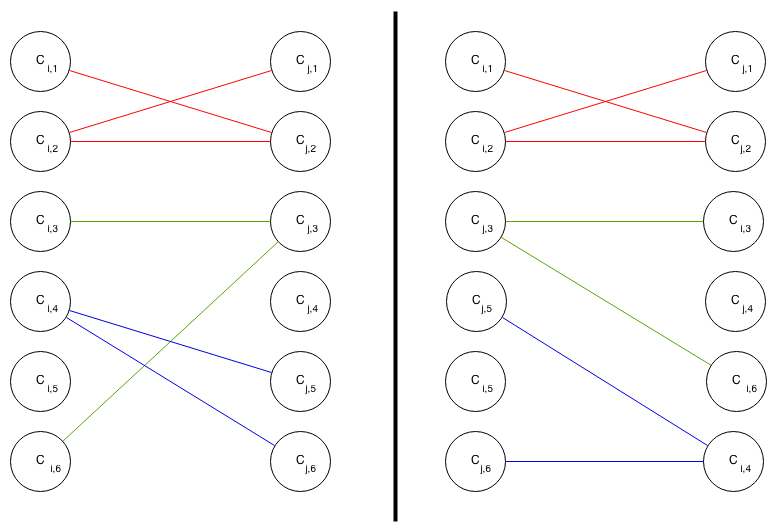
\includegraphics[height=10cm]{kempeSwap.png}\hfill
\centering

$t_i$\hspace{4.5cm}$t_j$\hspace{3.25cm}$t_i$\hspace{4.5cm}$t_j$ \\

\caption{Przykładowa zamiana łańcuchów Kempe: zielonego ($K_d$) i niebieskiego ($K_e$) dla okresów $t_i$ i $t_j$}
\label{fig:kempe_swap}
\end{figure}

\subparagraph{Przykład} 
Na rysunku \ref{fig:kempe_swap} po lewej stronie przedstawiono podgraf $G$, którego wierzchołkami są zajęcia, które zostały przydzielone do okresów $t_i$ i $t_j$, a krawędzie przedstawiają konflikty między kursami, do których należą te zajęcia. W podgrafie można wyróżnić 5 łańcuchów Kempe: $K_a = \{c_{i1}, c_{i2}, c_{j1}, c_{j2}\}$, $K_b = \{c_{i5}\}$, $K_c = \{c_{j4}\}$, $K_d = \{c_{i3}, c_{i6}, c_{j3}\}$, $K_e = \{c_{i4}, c_{j5}, c_{j6}\}$. Przykładowa zamiana dla łańcuchów $K_d$ i $K_e$ tworzy nowe przypasowanie (na rysunku \ref{fig:kempe_swap} po prawej stronie) przez przydzielenie $\{c_{i3}, c_{i4}, c_{i6}\}$ do $t_j$ i $\{c_{j3}, c_{i4}, c_{i6}\}$ do $t_i$.

\subparagraph{}Tak określony ruch można traktować jako rozszerzoną wersję podstawowej struktury sąsiedztwa, gdzie zamieniamy po kilka przypasowań na raz. Przy zamianie musimy uważać, aby nie wykonywać ruchów, które powodują przypasowanie do przedziałów czasowych większej liczby kursów, niż jest dostępnych sal. Dodatkowo nakładamy ograniczenia na liczbę kursów biorących udział w zamianie, tj. $|K_1|+ |K_2| \geq 3 $

%- room assignment
\par Po dokonaniu zamian w planie zajęć za pomocą łańcuchów Kempe następuje przypasowanie odpowiedniej sali do poszczególnych zajęć z danego okresu. Sale są przyporządkowywane do kursów metodą zachłanną, w każdym kroku wybieramy kurs, który nie ma przypisanej sali i jest kursem na który uczęszcza najwięcej studentów. Przypisujemy do kursu największą dostępną salę, sala zostaje oznaczona jako niedostępna.

\end{enumerate}
\paragraph{Lista tabu} służy do przechowywania informacji o ruchach tabu - ruchach, które nie mogą być wykonane przez określoną w tabu tenure dla kursu $c_{i}$ liczbę iteracji.
%-  dokłady opis tabu list
\subparagraph{}W przypadku sąsiedztwa prostego, jeśli zajęcia z kursu $c_i$ zostały przeniesione z okresu $t_j$ i sali $r_k$ w inne miejsce, wtedy przeniesienie jakichkolwiek zajęć z kursu $c_i$ do przedziału czasowego $t_j$ i sali $r_k$ przez kolejne $tt$ iteracji jest ruchem tabu. Podobnie dla sąsiedztwa zaawansowanego, jeśli zajęcia z kursu $c_i$ zostały przeniesione z przedziału czasowego $t_j$ do jakiegoś innego, wtedy przeniesienie jakichkolwiek zajęć z kursu $c_i$ do przedziału czasowego $t_j$ przez kolejne $tt$ iteracji jest ruchem tabu.\\

\subparagraph{Funkcja określająca liczbę iteracji, przez które ruch jest pamiętany na liście tabu} $tt(c_{i})$ obliczana jest na podstawie obecnie uzyskanego rozwiązania oraz częstotliwości przenoszenia zajęć z kursu $c_{i}$ oznaczonej przez $freq(c_{i})$. \\
Funkcję określono poniższym wzorem: 
 \[tt(c_{i}) = funkcja\ kary\ dla\ obecnego\ rozwiązania + \alpha * freq(c_{i}) \] 
gdzie ${\alpha = \frac{liczba\ konfliktujących\ kursów\ z\ c_{i}}{liczba\ kursów}}$ wobec tego wartość parametru ${\alpha \in [0, 1]}$ \\
gdyż ${liczba\ kursów \geq liczba\ konfliktujących\ kursów\ z\ c_{i}} $
\subparagraph{}Dzięki wprowadzeniu funkcji $tt(c_i)$ zróżnicowano czas, przez jaki różne ruchy są pamiętane na liście tabu. Ruchy wykonywane na początku przeszukiwania (kiedy funkcja kosztu jest wysoka) są pamiętane dłużej. Wprowadzenie czynnika zależnego od częstotliwości przenoszenia zajęć ma na celu przeciwdziałanie wielokrotnemu przenoszeniu zajęć tego samego kursu w to samo miejsce.

\paragraph{Procedura Tabu Search dla Adaptacyjnego Przeszukiwania Tabu}
\hfill
\begin{algorithm}[H]
    
    \begin{algorithmic}
    \STATE{$rozwiazanie_{najlepsze} = rozwiazanie_{aktualne}$}
    \WHILE{\emph{nie jest spełniony warunek stopu}}
    \STATE{$rozwiazanie_1 = tabu\_search\_proste\_sasiedztwo(rozwiazanie_{aktualne}, \theta)$}
    \STATE{$rozwiazanie_2 = tabu\_search\_zaawansowane\_sasiedztwo(rozwiazanie_1, \frac{\theta}{3})$}
    \IF	{$jakość(rozwiazanie_2)<jakość(rozwiazanie_{najlepsze})$}
    \STATE $rozwiazanie_{najlepsze} = rozwiazanie_2$
    \STATE $rozwiazanie_{aktualne} = rozwiazanie_2$
    \ENDIF

    \ENDWHILE
    \caption{Procedura $Tabu~search(rozwiazanie_{aktualne}, \theta)$}
    \label{tabusearch_tokenring}
    \end{algorithmic}
    \end{algorithm}
\par W algorytmie \ref{tabusearch_tokenring} $\theta$ oznacza głębokość przeszukiwania procedur $tabu\_search$ dla sąsiedztwa prostego i zaawansowanego.
\subsubsection{Faza dywersyfikacji}
\par Jeżeli rozwiązanie nie może zostać poprawione za pomocą algorytmu Tabu Search z \ref{tabusearch_tokenring} uruchamiana jest trzecia faza - faza dywersyfikacji. Głównym jej elementem jest losowy operator zaburzeń mający na celu opuszczenia osiągniętego lokalnego minimum. Początkowo identyfikowane są zajęcia z wysoką karą wynikającą z funkcji oceny  i losowo wybierane są zajęcia dla których zostaną dokonane zamiany sprecyzowane w poprzedniej fazie.
\par W momencie zakończenia fazy intensyfikacji, poszczególne zajęcia ustawiane są w kolejności malejącej ze względu na wysokość funkcji oceny. Z puli $q$ pierwszych zajęć wybierane jest $n$ zajęć, gdzie zajęcie będące na $k$ miejscu w rankingu wybierane zgodnie z normalizowanym rozkładem $P(k) = k^{-4.0}$. Następnie dokonywane jest $n$ losowych zamian pomiędzy zajęciami (sprecyzowanych w fazie intensyfikacji), ale tylko takich które zawierają przynajmniej jedno z wybranych z rankingu zajęć. \\
Przykład dla parametrów $q = 5$ i $n = 3$:
\begin{enumerate}
\item Po obliczeniu funkcji kary dla poszczególnych zajęć - ustawiamy zajęcia w kolejności nierosnącej pod względem funkcji kary (w $[\ ]$ podano przykładowe wartości funkcji kary)\\
\begin{enumerate}
 \item[(1)] $(t_{4}, fizyka, sala1)[127]$
 \item[(2)] $(t_{3}, religia, sala1)[89]$
 \item[(3)] $(t_{3}, język\ polski, sala2)[88]$
 \item[(4)] $(t_{4}, etyka, sala2)[80]$
 \item[(5)] $(t_{4}, język\ angielski, sala3)[77]$
 \item[(6)] $(t_{1}, język\ angielski, sala3)[52]$
 \item[(7)] $(t_{1}, biologia, sala2)[40]$
 \item[(8)] $(t_{2}, matematyka, sala2)[34]$
 \item[(9)] $(t_{2}, historia, sala1)[25]$
\end{enumerate}
\item Z puli wszystkich przedmiotów wybieramy $q = 5$ przedmiotów czyli przedmioty $(1) - (5)$ 
\item Rozkłady przed normalizacją dla wybranych $q$ zajęć:
	\begin{enumerate}
	\item[(1)] $P(1) = 1^{-4.0} = 1$
 	\item[(2)] $P(2) = 2^{-4.0} = \frac{1}{16}$
 	\item[(3)] $P(3) = 3^{-4.0} = \frac{1}{81}$
 	\item[(4)] $P(4) = 4^{-4.0} = \frac{1}{256}$
 	\item[(5)] $P(5) = 5^{-4.0} = \frac{1}{625}$
	\end{enumerate}
\item Losowane jest bez powtórzeń $n = 3$ zajęć zgodnie z powyższym rozkładem po dokonaniu normalizacji \\
	Przykłady wylosowanych zajęć [*]:
	\begin{enumerate}
	 \item[(1)] $(t_{4}, fizyka, sala1)[127]$
	 \item[(2)] $(t_{3}, religia, sala1)[89]$
	  \item[(4)] $(t_{4}, etyka, sala2)[80]$
	\end{enumerate}
\item Dla każdego z zajęć losujemy typ zamiany: podstawowa zamiana lub Kempe oraz znajdujemy wszystkie wykonywalne zamiany dla tego typu. Losowo wybieramy zamianę i przeprowadzamy ją. Odznaczając zajęcia, które są na liście [*], a dla których została już wykonana zamiana zawierająca te zajęcia.
\end{enumerate}




\subsection{Szczegóły implementacyjne}
\subsubsection{Struktury danych}
\paragraph{} Na potrzeby implementacji algorytmu plan zajęć został zamodelowany przy użyciu podstawowych struktur danych z języka Python. W pierwotnej wersji miał postać słownika, którego kluczami były kolejne numery przedziałów czasowych, a wartościami były listy, które przechowywały obiekty przypasowań zawierające identyfikatory kursu i sali. W trakcie implementacji okazało się, że kopiowanie takiej struktury wymaga korzystania z metody \verb#deepcopy# z modułu \verb#copy#, która przy wielu wywołaniach i dużej strukturze danych okazała się być nieefektywna. Ta obserwacja spowodowała, że w ostatecznej wersji obiekty przypasowań zastąpiono wbudowanym typem \verb#tuple#.
\subsubsection{Funkcja kosztu}
\paragraph{} Pomimo rozbudowanej matematycznej definicji funkcji kosztu w literaturze, efektywna implementacja okazała się być nietrywialna. Pierwsza wersja implementacji potrzebowała przejrzeć cały plan zajęć dla każdego ograniczenia miękkiego, w wersji ostatecznej wystarczą do tego tylko 2 przeglądy. Optymalizacja funkcji kosztu jest kluczowa dla czasu działania algorytmu. Korzystając z narzędzi do profilowania - moduł \verb#line_profile# - zauważyliśmy, że zdecydowaną większość czasu algorytm przeznacza na wykonanie funkcji kosztu.
\subsubsection{Optymalizacje językowe}
\paragraph{} Implementując algorytm staraliśmy się korzystać z funkcjonalnego paradygmatu programowania - funkcji \verb#map# i \verb#filter#, które w porównaniu ze zwykłymi pętlami w Pythonie nie mają dodatkowego narzutu przy iterowaniu. Ponadto korzystanie z elementów programowania funkcjonalnego spowodowało, że kod źródłowy jest w naszej ocenie bardziej zwięzły i czytelny.
\subsubsection{Test-Driven Development}
\paragraph{} Przy implementacji algorytmu staraliśmy wykorzystywać podejście TDD, czyli pisanie testów jednostkowych dla funkcji przed implementacją funkcji. ,,Szczelne'' pokrycie testami jednostkowymi podstawowych funkcji zdecydowanie ułatwiło późniejsze większe zmiany w logice i strukturze algorytmu.




\section{Particle Swarm Optimization (PSO)}
\author{Paweł Jastrzębski}
\subsection{Ogólny opis algorytmu}
\par Particle Swarm Optimaliation (PSO) lub optymalizacja rojem cząsteczek jest algorytmem zaproponowanym przez Jamesa Kennedy'ego oraz Russela Eberhart'a w roku 1995. Jest to technika wzorowana na zachowaniach występujących w przyrodzie. Algorytm naśladuje inteligencje i sposób poruszania się roju owadów poszukujących pożywienia. 
\par Zachowania te są w pewien sposób upraszczane, zamiast roju owadów mamy pewną liczbę cząsteczek (agentów) poruszających się w n-wymiarowej przestrzeni. Cząsteczki przemieszczają się w różnych kierunkach poszukując optymalnego rozwiązania. Korzystają przy tym ze swoich indywidualnych doświadczeń jak i doświadczenia ogółu.
\subsection{Działanie algorytmu}
\subsubsection{Oryginalna wersja}
\par W podstawowej wersji algorytmu używane są:
\begin{description}
  \item[Rój] \hfill \\
      Który posiada:
    \begin{itemize}
      \item Cząsteczki 
      \item Najlepszą pozycję (najlepsza pozycja osiągnięta dotychczas przez cząsteczki)
    \end{itemize}
  \item[Cząsteczki] \hfill \\
      Mające cechy:
    \begin{itemize}
      \item Pozycja (aktualna pozycja cząsteczki)
      \item Prędkość (wektor definiujący zmianę pozycji)
      \item Najlepsza pozycja (najlepsza pozycja osiągnięta przez tą konkretną cząsteczkę)
    \end{itemize}
\end{description}
\par Przebieg algorytmu można opisać poniższymi krokami:
\begin{description}
  \item[Krok 1:] 
     \par Stworzenie cząsteczek. Polega ono na ustawieniu ich pozycji i prędkości w sposób losowy. 
  \item[Krok 2:]
    \par Obliczenie prędkości dla każdej cząsteczki z osobna. 
  \item[Krok 3:]
        \par Zmiana pozycji każdej cząsteczki zgodnie z jej prędkością.
  \item[Krok 4:]
        \par Wyliczenie wartości funkcji dla aktualnych pozycji cząsteczek.
  \item[Krok 5:] 
      \par Sprawdzanie czy któraś cząsteczka poprawiła najlepszą pozycję roju lub samej siebie. Jeśli tak to aktualizujemy odpowiednią najlepszą pozycję.

\end{description}
    \par Kroki 2 - 5 są powtarzane aż do osiągnięcia wystarczająco dobrego wyniku lub maksymalnej liczby iteracji.
\subsubsection{PSO w problemie układania planu}
\par Modyfikacja PSO przedstawiona w tym rozdziale została zaczerpnięta z pracy ,,Timetable Scheduling Using Particle Swarm Optimization'' \cite{pso}
\par W tym podejściu każda cząsteczka posiada dwa kompletne plany zajęć. Jeden z nich jest przeznaczony do modyfikacji w każdej iteracji algorytmu (dalej nazywany planem aktualnym). Natomiast drugi plan jest używany do zapamiętywania dotychczas najlepszego planu znalezionego przez tą cząsteczkę (dalej nazywany lokalnie najlepszym planem). Obecny jest również globalny plan, którego zadaniem jest przechowywanie najlepszego planu znalezionego kiedykolwiek przez jakąkolwiek cząsteczkę (dalej nazywany globalnie najlepszym planem).  
\par Podczas każdej iteracji poszczególne cząsteczki będą poddawane trzem zmianom. Najpierw dwie losowe lekcje z planu aktualnego zostaną ze sobą zamienione. Potem jedna lekcja z lokalnie najlepszego planu zostanie skopiowana do aktualnego planu. Na koniec skopiujemy jedną lekcje z globalnie najlepszego planu do aktualnego planu. Kopia lekcji z innego planu wykonywana jest w następujący sposób. Wybierana jest lekcja z innego planu. Odszukujemy miejsce gdzie jest ta lekcja w aktualnym planie. Zamieniamy odszukaną lekcje z lekcją, która jest w miejscu do którego chcemy ją skopiować. 
\par Cały algorytm zaczynamy od stworzenia populacji dwudziestu cząsteczek. Każda z nich będzie posiadała losowo wygenerowany plan zajęć. Następnie dla każdej iteracji na każdej cząsteczce wykonywane będą poniższe kroki:
\begin{description}
  \item[Krok 1] \hfill \\
     \par Ocena rozwiązania. \hfill \\
   \par Oceniany zostaje aktualny plan. W tym momencie następuje aktualizacja lokalnie najlepszego planu oraz globalnie najlepszego planu.
  \item[Krok 2] \hfill \\
     \par Lokalna zamiana lekcji. \hfill \\
    \par Wykonana zostaje losowa zamiana dwóch lekcji w aktualnym planie.

  \item[Krok 3] \hfill \\
      \par Kopia lekcji z lokalnie najlepszego planu. \hfill \\
        \par Losowo wybrana lekcja z lokalnie najlepszego planu zostaje skopiowana do aktualnego planu 
  \item[Krok 4] \hfill \\
      \par Kopia lekcji z globalnie najlepszego planu. \hfill \\
        \par Losowo wybrana lekcja z globalnie najlepszego planu zostaje skopiowana do aktualnego planu 
\end{description}
\par Iteracje powtarzamy do czasu aż nie osiągniemy wystarczająco dobrego planu lub osiągniemy maksymalną liczbę iteracji albo skończy się nam limit czasu.
\subsection{Ścieżka dojścia do ostatecznego rozwiązania}
\subsubsection{Problem z proponowanym rozwiązaniem}
\par Podczas testowania proponowanego rozwiązania wystąpił problem. Algorytm wykazał się słabą skutecznością i nie był w stanie usunąć całkowicie problemów związanych z ograniczeniami "twardymi". Jak wiemy z rozdziału drugiego ograniczania "twarde" w ostatecznym rozwiązaniu nie mają prawa być łamane.
\par Aby algorytm brał pod uwagę w pierwszej kolejności ograniczenia "twarde", kary przydzielane za ich łamanie są mnożone przez milion.
Poniższy wykres pokazuje efektywność algorytmu. Uwagę należy zwrócić na skalę przyjętą na osi y. Wartości nie schodzą poniżej $10^{7}$ czyli wynik w najlepszym wypadku nadal łamie 10 ograniczeń "twardych".
\begin{figure}[H]
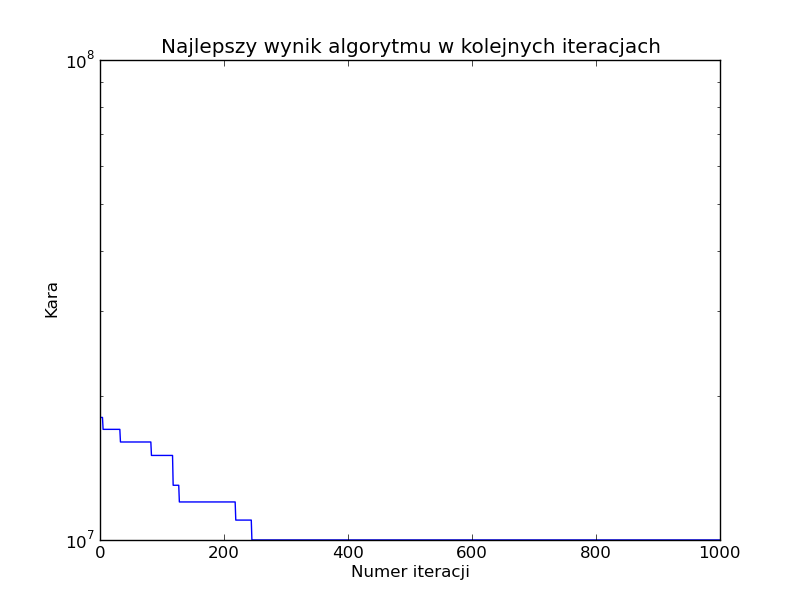
\includegraphics[width=10cm]{img/standard_penalty.png}
\centering
\end{figure}
\par Aby sprawdzić co się dzieje przyjrzałem się zachowaniu pojedynczej cząsteczki. Okazało się, że kara za kolejno generowane plany oscyluje wokół kary wyliczonej dla początkowego planu. Pokazuje to poniższy wykres.  
\begin{figure}[H]
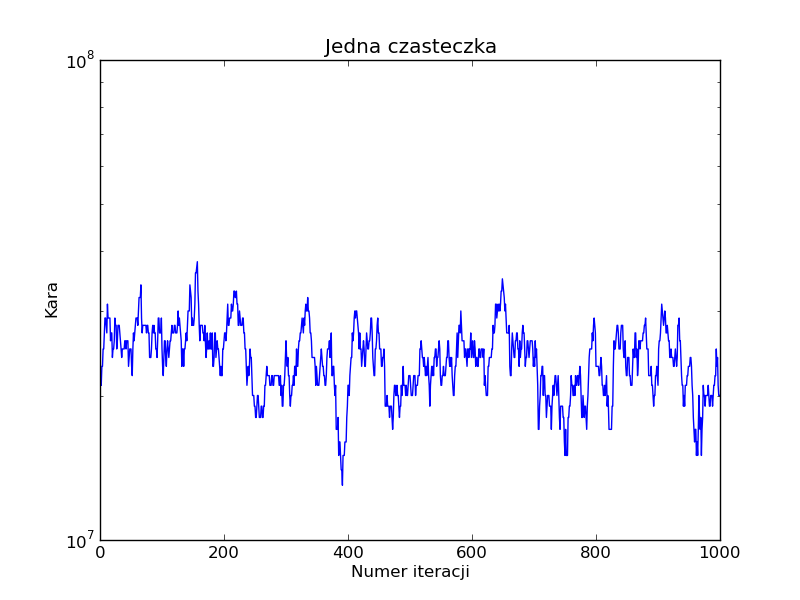
\includegraphics[width=10cm]{img/standard_particle.png}
\centering
\end{figure}
\par Na podstawie dalszej analizy okazało się, że wszystkie cząsteczki zachowują się bardzo podobnie. Widać to na poniższym wykresie.
\begin{figure}[H]
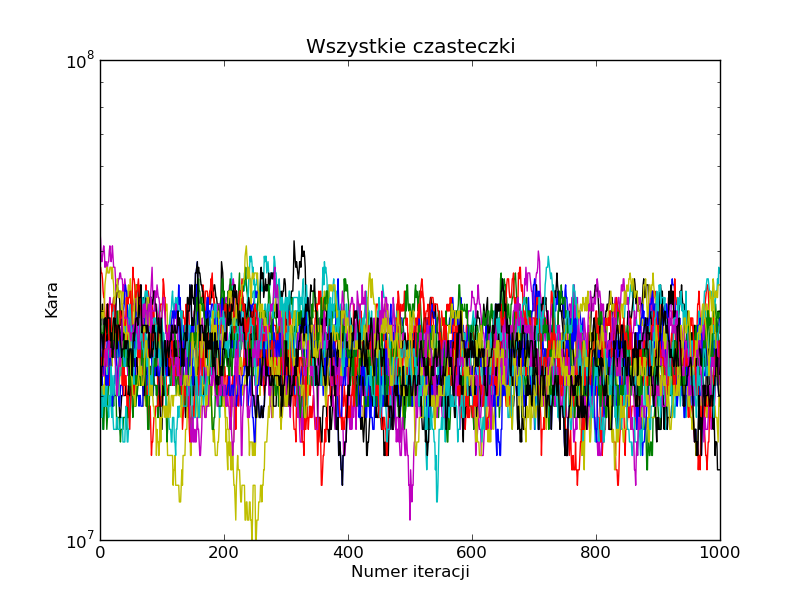
\includegraphics[width=10cm]{img/standard_particle_all.png}
\centering
\end{figure}
\subsubsection{Rozważane modyfikacje}
\par Rozważyłem dwie modyfikacje do aktualnego algorytmu. Jedną nazwałem podążaniem za lokalnie najlepszym planem, a drugą podążanie za globalnie najlepszym planem. Obie modyfikacje są względem siebie analogiczne, a różnią się tylko tym który plan bierzemy pod uwagę. Modyfikacją została objęta faza oceny aktualnego rozwiązania, która zachodzi na początku każdej iteracji. Dodany został warunek, że jeśli aktualny plan jest gorszy od najlepszego planu to zostaje on zamieniony na najlepszy plan. Usunięte też zostały kroki 3 i 4 czyli kopie z najlepszych planów.
\par W przypadku gdy każda cząsteczka podąża za swoim lokalnie najlepszym planem istnieje mniejsze ryzyko, że algorytm utknie w minimum lokalnym przestrzeni rozwiązań. Natomiast podczas podążania za globalnie najlepszym planem algorytm będzie znacznie szybciej dążył do najbliższego minimum.
\par Opcja podążania za lokalnie najlepszym planem okazała się być dużo efektywniejsza od podstawowego algorytmu. W tym przypadku ograniczenia "twarde" nie stanowiły problemu. Można to zobaczyć na poniższym wykresie.
\begin{figure}[H]
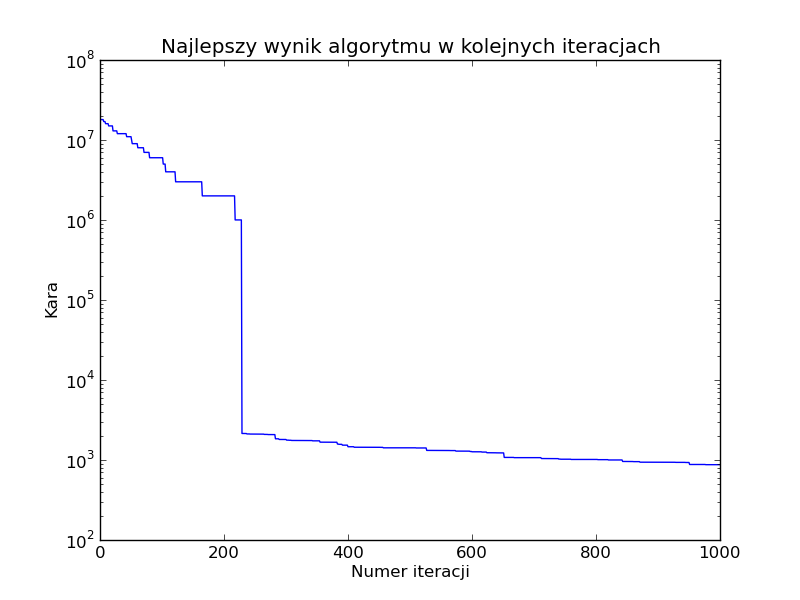
\includegraphics[width=10cm]{img/localbest_penalty.png}
\centering
\end{figure}
\par Analizując pojedynczą cząsteczkę można zauważyć, że często kara skacze od małych wartości do wartości milionowych. Jest to spowodowane tym, że w po zamianie dwóch lekcji w poprzedniej iteracji pojawił się konflikt z ograniczeniami "twardymi". Nie stanowi to problemu, ponieważ w takim przypadku wracamy do poprzedniego rozwiązania. Na poniższych wykresach widać zachowanie dla pojedynczej cząsteczki oraz dla wszystkich cząsteczek.
\begin{figure}[H]
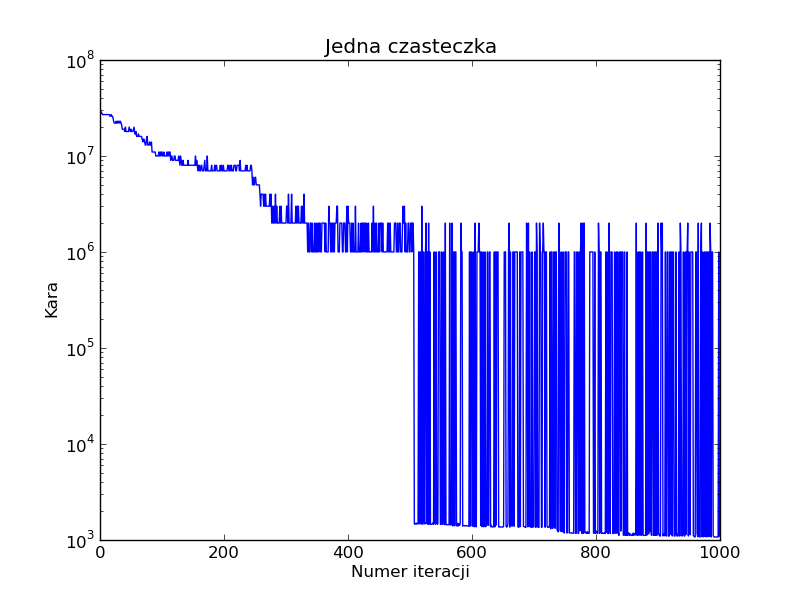
\includegraphics[width=10cm]{img/localbest_particle.png}
\centering
\end{figure}
\begin{figure}[H]
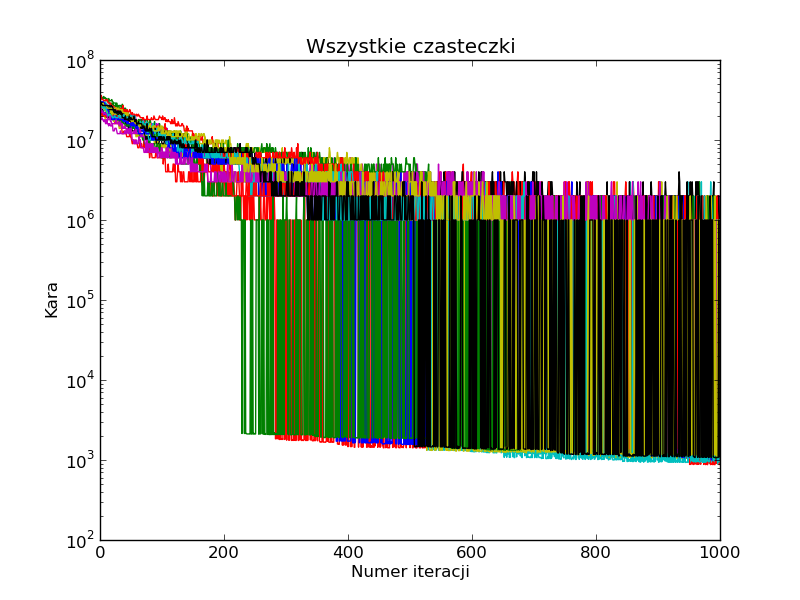
\includegraphics[width=10cm]{img/localbest_particle_all.png}
\centering
\end{figure}
\par Opcja podążania za globalnie najlepszym planem okazała się jeszcze bardziej efektywna. Sporym zaskoczeniem był brak problemów z lokalnymi minimami przestrzeni rozwiązań. Poniższy wykres pokazuje skuteczność modyfikacji.
\begin{figure}[H]
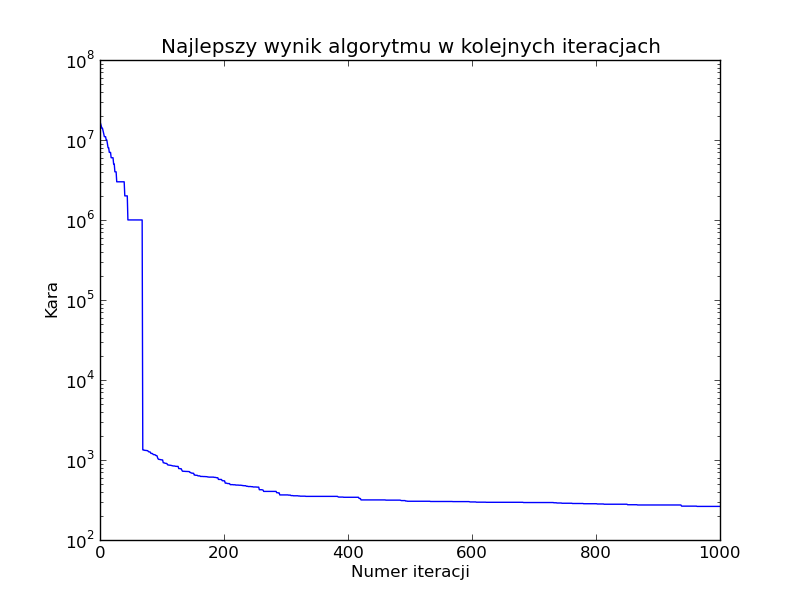
\includegraphics[width=10cm]{img/globalbest_penalty.png}
\centering
\end{figure}
\par W tym przypadku cząsteczki zachowywały się bardzo podobnie. Jedyną różnicą była prędkość z jaką spadała kara. Widać to na poniższych wykresach. 
\begin{figure}[H]
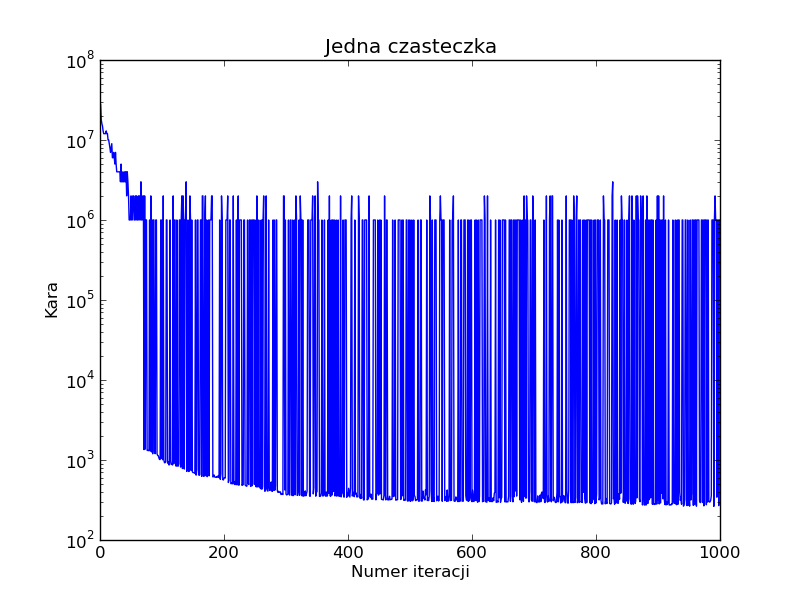
\includegraphics[width=10cm]{img/globalbest_particle.png}
\centering
\end{figure}
\begin{figure}[H]
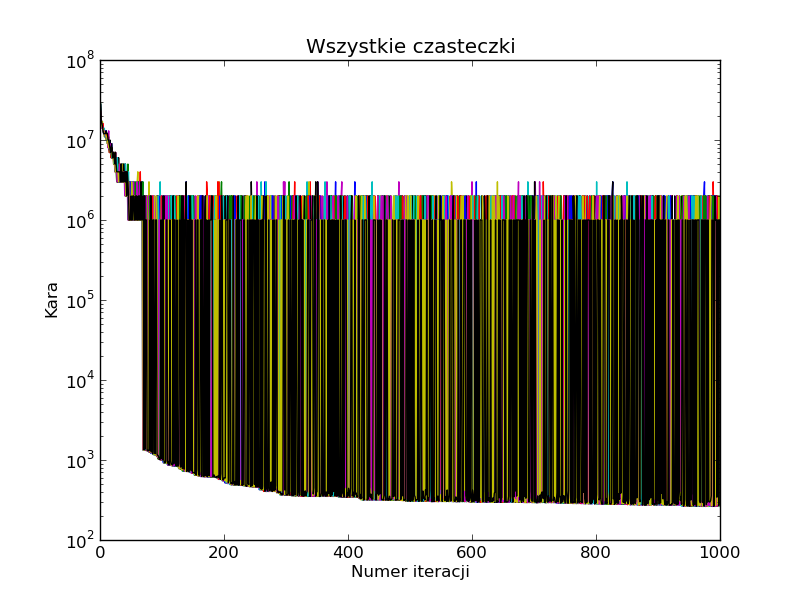
\includegraphics[width=10cm]{img/globalbest_particle_all.png}
\centering
\end{figure}
\subsubsection{Ostateczne rozwiązanie}
\par Jako ostateczne rozwiązanie wybrałem podążanie za globalnie najlepszym planem. Jest to spowodowane tym, że mimo wielu testów nie udało mi się znaleźć przypadku kiedy podążanie za lokalnie najlepszym planem wypadłoby lepiej. 

\section{Genetic Algorithm (GA)}
\author{Filip Czajkowski}
\subsection{Ogólny opis algorytmu}
\par Algorytm genetyczny jest heurystyką poszukującą rozwiązania problemu, która naśladuje proces naturalnej selekcji w procesie ewolucji. W informatyce należy do szerszej grupy algorytmów ewolucyjnych i zawiera się w dziedzinie sztucznej inteligencji. Jego działanie opiera się na przeszukiwaniu przestrzeń alternatywnych rozwiązań w problemach optymalizacyjnych w celu wyszukania rozwiązań najlepszych. Cały algorytm operuje na grupie (populacji) potencjalnych rozwiązań, których jakość (stopień, w jakim jest bliskie rozwiązania optymalnego) potrafimy ocenić i które zbliżają się w przypominającym ewolucyjny procesie do rozwiązania optymalnego. Tym, co go wyróżnia jest zastosowanie operacji zaczerpniętych z genetyki, takich jak selekcja, krzyżowanie czy mutacja.
\par Algorytmy genetyczne zajmują bardzo ważne miejsce w dziedzinie projektowania i analizy algorytmów. Doskonale sprawdzają się w sytuacji, gdy problem, z którym przychodzi nam się zmierzyć, jest nie do rozwiązania w sposób klasyczny w sensownym czasie. Pozwalają znaleźć sub-optymalne rozwiązanie problemów, których dziedziny nie są łatwe do wyznaczenia. Są powszechnie stosowane tam, gdzie do uzyskania rozwiązania korzystamy z zagadnień sztucznej inteligencji oraz tam, gdzie uzyskanie rozwiązania jest bardzo złożonym problem, natomiast jego ocena jest łatwa i błyskawiczna. Należy zaznaczyć, że algorytm genetyczny nie gwarantuje znalezienia rozwiązania optymalnego, lecz przybliżone. Dla żadnej ilości iteracji lub liczby osobników nie ma pewności, że algorytm osiągnie optymalne rozwiązanie. W zależności od implementacji istnieje większe lub mniejsze ryzyko, iż algorytm utknie w lokalnym minimum i nie będzie w stanie w pełni wyeksplorować przestrzeń rozwiązań. Z tego powodu w bardzo złożonych problemach niemal pewne jest, iż globalne maksimum nie zostanie osiągnięte. Dlatego też zastosowanie tego algorytmu wciąż się zawęża, gdyż wraz z powstawaniem rozwiązań dedykowanych dla konkretnych problemów, algorytm ten najczęściej okazuje się od nich mniej wydajny. Wciąż jednak pozostaje wiele zagadnień, dla których świat nauki nie znalazł jeszcze specjalistycznego rozwiązania, a w takich przypadkach algorytm genetyczny ciągle pozostaje w gronie heurystyk, które stają się pomocne.
\par Problem definiuje środowisko, w którym istnieje pewna populacja osobników. Każdy z nich posiada zestaw informacji, które tworzą określone struktury.
\begin {itemize}
\item \textbf{Genotyp} - przypisany każdemu osobnikowi ogólny zbiór informacji, które tworzą proponowane rozwiązanie oraz są podstawą do utworzenia fenotypu.
\item \textbf{Fenotyp} - to zbiór cech podlegających ocenie funkcji przystosowania modelującej środowisko, zatem określenia, jak dobre jest dane rozwiązanie.
\item \textbf{Chromosom} - to tutaj zakodowany jest fenotyp i ewentualnie dodatkowe informacje pomocnicze dla procesu tworzenia rozwiązania.
\item \textbf{Gen} - Pojedyncza jednostka informacji, z których zbudowany jest chromosom.
\end{itemize}
\par Schemat działania algorytmu prezentuje się w następujący sposób:
\begin{enumerate}
\item Losowana jest pewna populacja początkowa, każdy osobnik przydzielane ma wygenerowane w sposób możliwie losowy przykładowe rozwiązanie.
\item Populacja poddawana jest ocenie (selekcja). Najlepiej przystosowane osobniki biorą udział w procesie reprodukcji.
\item Wybrane osobniki biorą udział w etapie reprodukcji, który odbywa się poprzez  złączanie genotypów dwójki rodziców (krzyżowanie).
\item Przeprowadzana jest mutacja, czyli wprowadzenie drobnych losowych zmian u niektórych osobników.
\item Rodzi się kolejne pokolenie. Aby utrzymać stałą liczbę osobników w populacji te najlepsze według funkcji oceny przystosowania są powielane, a najsłabsze usuwane. Jeżeli nie znaleziono dostatecznie dobrego rozwiązania, algorytm powraca do kroku drugiego. W przeciwnym wypadku wybieramy najlepszego osobnika z populacji - jego genotyp to uzyskany wynik.
\end{enumerate}
\subsection{Historia i zastosowanie}
Sposób działania algorytmów genetycznych nieprzypadkowo przypomina zjawisko ewolucji biologicznej, ponieważ ich twórca John Henry Holland właśnie z biologii czerpał inspiracje do swoich prac. W 1975 roku wydał książkę \emph{"Adaptation in Natural and Artificial Systems"}, w której jako pierwszy wykazał, jak procesy genetyczne mogą mieć zastosowanie wśród rozwiązywania problemów optymalizacyjnych. Specyfika działania algorytmu czyni go bardzo uniwersalnym. Możliwości jego użycia wybiegają poza czystą algorytmikę i znajduje on zastosowanie w bioinformatyce, inżynierii, ekonomii, chemii, matematyce czy fizyce. Konkretnymi przykładami mogą być np. poszukiwanie najbardziej aerodynamicznego kształtu skrzydła samolotu, opracowanie kształtu anteny najlepiej odbierającej fale radiowe albo, tak jak w tym przypadku, problem układania planu zajęć.
\subsection{Fazy algorytmu w implementowanym rozwiązaniu}
\par Opisywany wcześniej schemat działania algorytmu należy przełożyć na problem układania planu zajęć i zdefiniować schematy danych a następnie operacje na nich wykonywane. Poniższa tabela ilustruje jak obiekty ze świata genetyki odwzorowują opisywany problem.
\begin{center}
\begin{tabular}{| l | p{10cm} |}
\hline
populacja & zbiór wszystkich planów zajęć \\ \hline
osobnik & pojedynczy rozkład zajęć wraz z ograniczeniami \\ \hline
genotyp & rozkład zajęć wszystkich kursów \\ \hline
funkcja przystosowania & funkcja oceny planu względem założeń \\ \hline
fenotyp & realna wartość rozwiązania \\ \hline
chromosom & tablica, której indeksy stanowią dostępne przedziały czasowe, a wartości to listy odbywających się wówczas zajęć w postaci pary (pomieszczenie, kurs) \\ \hline
gen & przyporządkowanie w tablicy o identyfikatorze "czas" pary  (pomieszczenie, kurs) \\ \hline
\end{tabular}
\end{center}
\subsubsection{Utworzenie rozwiązania początkowego}
\par Etap ten jest bardzo złożony i polega na stworzeniu przykładowego rozwiązania dla każdego osobnika populacji. Powinny one się różnić między sobą, lecz nie koniecznie muszą spełniać wszystkie twarde ograniczenia. Ponieważ niespełnianie podstawowych warunków jest sankcjonowane bardzo dużymi karami, w procesie ewolucji rozwiązania te zostaną wyparte lub poprawione.
\par Zatem dla każdego osobnika należy przyporządkować wszystkie zajęcia do jakichkolwiek sal i przedziałów czasowych starając się jednocześnie nie naruszać twardych ograniczeń. Losowana jest wpierw kolejność kursów, których zajęcia będą kolejno przyporządkowywane. Dla każdej lekcji staramy się znaleźć czas i miejsce wedle jednej ze strategii:
\begin{enumerate}
\item Wybierz najmniejsze możliwe pomieszczenie, w którym zmieszczą się wszyscy uczestnicy kursu. Jeśli zajęcia należące do kursu nie odbywają się jeszcze w minimalną zakładaną ilość dni, szukaj wolnego terminu wśród pozostałych dni. Jeśli nie udało się, spróbuj z pomieszczeniem następnym w kolejności pod względem rozmiaru. Powtarzaj ten proces dopóki nie znajdziesz wolnego terminu lub nie sprawdzisz wszystkich pomieszczeń.
\item Podobnie jak w pierwszym przypadku, szukaj wolnych terminów dla pomieszczeń, w których pomieszczą się wszyscy studenci, lecz nie bierz pod uwagę dni, w które odbywają się zajęcia. Tutaj także szukamy wolnego terminu aż sprawdzimy wszystkie pomieszczenia, których pojemność jest niemniejsza niż ilość osób biorących udział w zajęciach.
\item Zastosowanie trzeciej strategii jest rozwiązaniem ostatecznym, ponieważ najczęściej wiąże się z naruszeniem twardych ograniczeń.  Wylosuj przedział czasowy i sprawdź, czy istnieje pokój, wolny pokój, który może pomieścić daną grupę. Nie bierz pod uwagę ograniczeń dostępności prowadzącego. W razie niepowodzenia, poszukaj jakiegokolwiek wolnego pomieszczenia w danym przedziale czasowym. Operacje te powtarzaj losując terminy aż znajdziesz wolny pokój.
\end{enumerate}
\par Ostatnią operacją do wykonania w tym kroku jest ocenienie wszystkich wygenerowanych rozwiązań i zapisaniu najlepszego wyniku. Proces ten sprowadza się do sprawdzenia naruszeń ograniczeń twardych i stopnia spełnialności ograniczeń miękkich poprzez nakładanie odpowiednich kar. W ten sposób najlepszym rozwiązaniem staje się to, dla którego suma kar jest najmniejsza.
\subsubsection{Selekcja}
Etap ten polega na dokonaniu wyboru, które osobnika zostaną poddane krzyżowaniu. Zaimplementowane w celu porównania zostały 3 metody selekcji:
\begin{enumerate}
\item \textbf{Selekcja losowa} - rozwiązanie to jest bardzo proste, a mianowicie polega na losowym wybraniu dwóch różnych od siebie osobników. Taki model powoduje, iż rozwiązania gorsze i słabsze mają taką samą szansę na reprodukcję, zatem nie sprzyja to tworzeniu coraz to lepszych potomków.
\item \textbf{Selekcja ruletkowa} - jej nazwa pochodzi od popularnej gry w ruletkę i sposób wyłaniania osobnika bardzo ją przypomina. Można ją zilustrować jako poruszenie "kołem fortuny", w którym każdemu osobnikowi przypisany jest wycinek, którego wielkość jest odwrotnie proporcjonalna do wartości funkcji przystosowania. Dzieję się tak, ponieważ chcemy aby osobniki o mniejszej wartości funkcji oceny miały większą szansę na wylosowanie.
\item \textbf{Selekcja turniejowa} - wyłanianie osobników do procesu krzyżowania odbywa się poprzez pewną formę konkursu. Losowanych jest kilku uczestników (ich ilość jest jednym z parametrów algorytmu, wartość nominalna to 4), a wybierany jest ten spośród nich, który jest najlepiej przystosowany do środowiska. Zawodnicy w danym turnieju oczywiście muszą być różni, lecz po przeprowadzeniu wielu takich rozgrywek, najlepsi z nich powinni zostać wybierani najczęściej.
\end{enumerate}
\par Etap selekcji zostanie przeprowadzony na połowie wszystkich uczestników, co oznacza, że krzyżowaniu zostanie poddana tylko połowa z nich.
\subsubsection{Krzyżowanie}
Proces ten polega na złączeniu w sposób losowy genotypu dwóch rodziców wybranych w poprzednim kroku w celu stworzenie potomka, który będzie dziedziczył po nich wszystkie cechy. Ilość materiału genetycznego każdego z rodziców powinna być jednakowa. W naszym rozwiązaniu, z danej pary rodziców tworzona jest dwójka dzieci będących początkowo kopiami swoich rodziców. Następnie część genotypu pierwszego dziecka jest zastępowana genotypem drugiego rodzica, a drugiemu dziecku wprowadzane są informacje dziedziczone po pierwszym rodzicu. Schemat krzyżowania w kontekście planu zajęć przestawia się w następujący sposób:
\begin{enumerate}
\item Tworzymy kopie rodziców \emph{child1 = mother} oraz \emph{child2 = father}
\item Losujemy kursy, których zajęcia zawarte u rodzica będą wprowadzane do drugiego dziecka w miejsce zajmowane w genotypie rodzica. Ponieważ nie wszystkie zajęcia będzie dało się przenieść tak, aby nie powodowały konfliktów, kryterium końca tego procesu będzie jakiekolwiek przeniesienie połowy sumarycznej ilości kursów.
\item 
\begin{itemize}
\item Dla każdego przenoszonego zajęcia sprawdź, czy dane zajęcia i odpowiadające mu zajęcie u dziecka są identyczne. W takim wypadku nic nie rób i oznacz zamianę jako udaną.
\item Jeśli pomieszczenie jest już zajęte, oznacz operację jako nieudaną.
\item Jeśli pomieszczenie jest wolne i wprowadzenie zajęć w tym terminie nie narusza żadnych ograniczeń twardych, to oznacz operację jako pozytywną, w przeciwnym razie jako negatywną.
\end{itemize}
\item Jeśli wynik poprzedniego kroku jest negatywny postępują według następujących scenariuszy:
\begin{itemize}
\item Jeśli gen, który chcemy wprowadzić nie jest pusty, to usuń jego dowolnego reprezentanta w genotypie dziecka.
\item Jeśli pomieszczenie jest wolne, spróbuj wprowadzić lekcję w wybranym terminie, pod warunkiem, że ta operacja nie narusza ograniczeń twardych. Jeśli się powiedzie, oznacz operację jako udaną, jeśli nie, podążaj dalej.
\item Spróbuj znaleźć inny termin z wolnym tym samym pokojem oraz dla którego operacja wprowadzenia genu nie powoduje konfliktów. W przypadku niepowodzenia, przejdź do kolejnego kroku.
\item Poszukuj jakichkolwiek wolnych pomieszczeń, w których mogą odbyć się dane zajęcia i szukaj dla niego wolnego terminu. Jeśli taka para się nie znajdzie, operacja zostaje ostatecznie oznaczona jako nieudana i należy spróbować ją powtórzyć dla innego kursu i zajęć.
\end{itemize}
\end{enumerate}
\par Cały opisany powyżej schemat zostaje powtórzony w analogiczny sposób dla drugiego dziecka. Umożliwia on losowe wymieszanie genów rodziców przy jednoczesnym zachowaniu ważności rozwiązania. Wiąże się to jednak z koniecznością długich poszukiwań terminów dla wprowadzanych genów. Z każdej pary rodziców powstaje dwójka potomstwa. Zgodnie z zasadami ewolucji, gdzie przetrwać mogą tylko najlepiej przystosowani, do następnego pokolenia przejdzie lepsza połowa osobników z poprzedniego pokolenia, która zostanie uzupełniona dziećmi powstałymi właśnie dziećmi.
\subsubsection{Mutacja}
Podobnie jak w naturalnym procesie mutacji, tutaj też polega on na wprowadzeniu losowych zmian w powstałym kompletnym potomku. Prawdopodobieństwo jego zajścia jest niewielkie (domyślnie 1\%), więc dotyczyć on będzie jednego bądź kilku genów. W tym przypadku skasowane zostaną wszystkie zajęcia z wybranego kursu i algorytm spróbuje na nowo je przyporządkować. Proces ten jest identyczny jak w przypadku generowania rozwiązania początkowego.
\subsubsection{Elityzm}
\par Jest to zagadnienie związane z etapem mutacji. Ponieważ rezultat tego działania może polepszyć lub pogorszyć wcześniejsze rozwiązanie, nie będziemy mu poddawać jednego (domyślnie) lub kilku najlepszych rozwiązań, aby nie utracić ich wyniku. Elityzmem nazywamy więc ochronę najlepszego rozwiązania przed możliwą regresją podczas mutacji.
\subsection{Istniejące implementacje}
\begin{itemize}
\item{FET - Free Evolutionary Timetable}
Jest to program darmowy, stworzony dla platformy Linux, rozpowszechniany na zasadach licencji GNU GPL. Napisany w C++ z wykorzystaniem biblioteki Qt, dane pobiera z plików w formacie XML. Rozbudowany interfejs umożliwia śledzenie procesu ewolucji.
\item{Tablix}
Jest to polski produkt typu \emph{open source}, jego autorem jest Tomasz Solc. Program powstał w technologii języka C z użyciem pakietu PVM, który umożliwia zrównoleglenie obliczeń, co znacząco przyspiesza działanie algorytmu. Dane wejściowe muszą znajdować się w plikach XML. Nie posiada natomiast interfejsu graficznego, który umożliwiałby edycję danych lub wizualizację wyników.
\end{itemize}



\chapter{Etapy przetwarzania danych szkolnych}
\textit{Katarzyna Śmietanka} \\
Ważnym etapem pracy nas systemem okazało się być przystosowanie algorytmów do realnych danych uzyskanych z jednej ze szkoł ponadgimnazjalnych. Proces ten wymagał przeprowadzenia różnych działań związanych z eksploracją danych, czyli przetworzenia danych oraz wyodrębnienia istotnych danych dla zdefiniowanego przez nas problemu. Na proces obróbki danych składało się kilka etapów: analiza danych, wybór istotnych danych, transformacje danych, czyszczenie i uzupełnienie brakujących danych oraz stworzenie wizualizacji danych.
\section{Opis danych szkolnych}
Uzyskane dane szkolne są plikami tekstowymi w formacie CSV. \\
W sekcji tej poniższe pojęcia będą używane synonimicznie: \\
kurs - przedmiot \\
program nauczania - klasa \\
Rodzaje plików z danymi:
\begin{enumerate}
\item[1.] Dla każdej klasy nauczane przedmioty oraz uczący nauczyciele.
\begin{verbatim}
Format:
<Nazwa przedmiotu><Prowadzący przedmiot>
\end{verbatim}
\item[2.] Grupy występujace w szkole
\begin{verbatim}
Format:
<Kod grupy> <Grupa nadrzędna> <Nazwa grupy> <Rodzaj grupy> 
<Opiekun grupy><Liczba uczniów><Rok szkolny><Status grupy>
<Inkrementować numer><Osoba wprowadzająca><Data wprowadzenia>
\end{verbatim}
\item[3.] Słownik godzin lekcyjnych
\begin{verbatim}
Format:
<ID>	<Nazwa><Godzina rozpoczęcia><Godzina zakończenia><Aktywny>
\end{verbatim}
\item[4.] Lista miejsc
\begin{verbatim}
Format:
<ID><Miejsce><Aktywny>
\end{verbatim}
\item[5.] Zestawienie planu
\begin{verbatim}
Format:
<Plan zajęć><Rok szkolny><Grupa uczniów><Cykl><Data zajęć>
<Okres cyklu od><Okres cyklu do><Termin><Godzina lekcyjna>
<Godzina rozpoczęcia> <Godzina zakończenia><Zajęcia><Miejsce><Prowadzący>
\end{verbatim}
\end{enumerate}
\section{Etapy przetwarzania danych}
\begin{figure}[H]
  \centering
    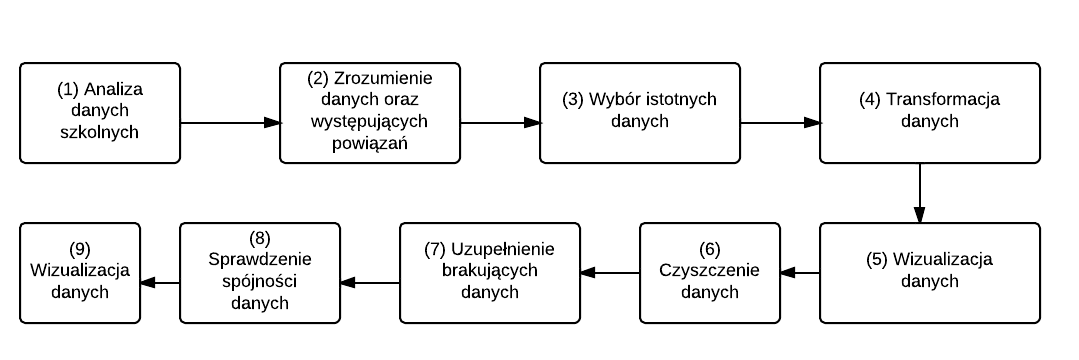
\includegraphics[width=0.8\textwidth]{proces_przetwarzania.png}
  \caption{Szkip etapów przetwarzania danych}
\end{figure}
\begin{enumerate}
\item[(1)] \textbf{Analiza danych szkolnych} - zapoznanie się z danymi oraz analiza w jaki sposób efektywnie i racjonalnie wykorzystać nagromadzoną wiedzę, poznanie struktury danych.
\item[(2)] \textbf{Zrozumienie danych oraz identyfikacja występujących powiązań} - szczegółowe poznanie zależności pomiędzy poszczególnymi danymi występującymi m.in. grupami uczniów a klasami, przedmiotami a nauczycielami prowadzącymi zajęcia.
\item[(3)] \textbf{Wybór istotnych danych} - wyodrębnienie istotnych danych niezbędnych do stworzenia wykonywalnego planu zajęć: klasy, przedmioty, które są nauczane w danej klasie, liczba uczniów uczestniczących w danych zajęciach, informacje o przedmiotach międzyklasowych, liczbie godzin realizowanego przedmiotu oraz prowadzących dany przedmiot.
\item[(4)] \textbf{Transformacja danych} - wykonane transformacje opisane w sekcji ,,Transformacje''
\item[(5)] \textbf{Wizualizacja danych} - wykonanie grafów przedstawiających zależności pomiędzy danymi, szczegółowy opis w sekcji ,,Wizualizacja danych szkolnych''
\item[(6)] \textbf{Czyszczenie danych}  - usunięcie niepełnych, niepoprawnych oraz nieistotnych danych np. kursy (przedmioty), które mają niepełne dane zaburzające działanie algorytmu, usunięcie zbędnych kursów m.in. $Biblioteka\ szkolna$, który w znacznym stopniu utrudniał ułożenie planu poprzez zwiększenie liczby konfliktów pomiędzy zajęciami.
\item[(7)] \textbf{Uzupełnienie brakujących danych} - dane uzyskane ze szkoły nie zawierały informacji o maksymalnej liczbie osób, która może się zmieścić w danej sali, typach sal szkolnych - co jest dość istotnym elementem, który wpływa na realność ułożonego planu. Nie uzwględnienie tego czynnika może powodować, że np. zajęcia z matematyki będą musiały odbywać się na sali gimnastycznej. 
\item[(8)] \textbf{Sprawdzenie spójności danych} - wczytanie danych do struktury początkowej dla zaimplementowanych algorytmów.
\item[(9)] \textbf{Wizualizacja danych} - w celu łatwiejszej identyfikacji występujących błędów oraz sprecyzowanie trudności ułożenia planu zajęć dla tych danych.
\end{enumerate}
\subsection{Transformacje}
Przetworzenie danych szkolnych do formatu konkursowego wymagało przeprowadzenia kilku transformacji danych, które zostały wymienione poniżej:
\begin{enumerate}
\item Odczytanie istniejących grup w szkole i przypisanie tych grup do poszczególnych klas, wyodrębnienie klas na podstawie \verb#<Grupa nadrzędna> <Nazwa grupy>#
\item Identyfikacja grup międzyklasowych z dokumentu ,, Zestawienie planu'' przy pomocy funkcji \verb#groupby()#  na podstawie wspólnych kluczy: 
\begin{verbatim}
<Termin><Godzina lekcyjna><Zajęcia>
	<Godzina rozpoczęcia><Godzina zakończenia><Prowadzący>
\end{verbatim}
Po reformie oświaty w szkołach ponadgimnazjalnych uczniowie uzyskali możliwość wyboru nauczanych przedmiotów na poziomie rozszerzonym, co spowodowało powstanie grup międzyklasowych realizujących ten sam przedmiot. \\
Jako, że grupy międzyklasowe nie posiadały jednego wspólnego identyfikatora, który był taki dla sam dla kilku klas, konieczne było przeprowadzenie operacji grupowania. \\
Przykład:
\begin{verbatim}
Dane z dokumentu "Zestawienie planu":
>>>2013/2014 Wrzesień;2013/2014 aktywny;2 LW Chemia;Tygodniowy;;
	2013-09-16;2014-01-31;Poniedziałek;Lekcja 1;08:00;08:45;
	Chemia CHEM;Sala 119;ŚaAa
>>>2013/2014 Wrzesień;2013/2014 aktywny;2 LP Chemia;Tygodniowy;;
	2013-09-16;2014-01-31;Poniedziałek;Lekcja 1;08:00;08:45;
	Chemia CHEM;Sala 119;ŚaAa
Występujące identyfikatory grup: 
2 LW Chemia
2 LP Chemia
\end{verbatim}
Pomimo różnych identyfikatorów można zauwazyć, że  grupy \verb#2 LW Chemia# oraz 
\verb#2 LP Chemia# tworzą jedną z grup międzyklasowych, ponieważ są nauczane przez tego samego nauczyciela oraz odbywają się dokładnie w tym samym czasie.
\item Przypisanie identyfikatorów grup międzyklasowych do odpowiednich klas (stworzenie międzyklasowych kursów), dla których dany przedmiot jest nauczany. Zliczenie liczby godzin realizowanego kursu międzyklasowego i liczby studentów uczęszczających na dany kurs.
\item Wyodrębnienie wszystkich przedmiotów nauczanych w szkole (nauczanych tylko w obrębie jednej klasy) oraz przypisanie ich do opowiednich klas.
\item Zgrupowanie danych z dokumentu ,,Zestawienie planu'' na podstawie kluczy: \\
\verb#<Zajęcia><Grupa uczniów># w celu zliczenia liczby godzin realizowanego przedmiotu w danej klasie oraz przypisania identyfikora nauczyciela. \\
Dokument ,,Zestawienie planu'' zawiera aktualnie ułożony plan szkolny, w którym każde zajęcia przyporządkowane są do dnia tygodnia i godziny lekcyjnej oraz klasy. Aby uzyskać liczbę godzin nauczanego przedmiotu lub liczbę uczniów, konieczne było przeprowadzenie operacji grupowania.
\end{enumerate}
\subsection{Specyfikacja uzyskanych danych}
\begin{table}[H]
\begin{center}

\begin{tabular}{ |c|c|c| }
\multicolumn{1}{r}{}
 &  \multicolumn{1}{c}{$$}
 & \multicolumn{1}{c}{$$} 
 \\
\cline{1-2}
$Liczba\ przedmiotów\ (kursów)$ & $373$\\
\cline{1-2}
$Liczba\ klas\ (programów\ nauczania)$ & $22$\\
\cline{1-2}
$Liczba\ dni$ & $5$ \\
\cline{1-2}
$Licza\ przedziałów\ czasowych$ & $15$ \\
\cline{1-2}
$Liczba\ ograniczeń$ & $0$ \\
\cline{1-2}
\end{tabular}
\end{center}
\caption {Opis przetworzonych danych}
\end{table}
Dla przypadku testowego ,,Dane szkolne'' nie zostały wprowadzone żadne ograniczenia, ponadto rozszerzono $Licza\ przedziałów\ czasowych$ z $11$ na $15$. \\
Uzasadnienie rozszerzenia liczby przedziałów czasowych: \\
Zaimplementowane przez nas algorytmy nie uwzględniają możliwości przydzielenia zajęć, które należącą do tego samego programu nauczania, do jednakowego przedziału czasowego w planie zajęć. Co w obecnej specyfikacji problemu byłoby jednoznaczne z naruszeniem ograniczeń twardych\\
Przykład wyjaśniający problem dla klasy o identyfikatorze \verb#2 LW#:
\begin{verbatim}
Do programu nauczania dla tej klas należą kursy:
2 LW WF Dziewczęta
2 LW WF Chłopcy
\end{verbatim}
Osoba układająca plan posiada wiedzę, które zajęcia będące w programie nauczania dla danej klasy mogą odbywać się w tym samym czasie. Konieczne jest tu sprawdzenie czy zbiory uczęszczających uczniów na te zajęcia są rozłączne oraz nauczane są przez innego nauczyciela. \\
Z uzyskanych danych nie jesteśmy w stanie jednoznacznie wywnioskować rozłączności zbiorów, choć intuicyjnie wydaje się to oczywiste dla przypadku przedmiotu: $Wychowanie\ fizyczne$, że grupy uczniów uczęszczających na zajęcia  \verb#2 LW WF Dziewczęta# i \verb#2 LW WF Chłopcy# są zbiorami rozłącznymi.
Mniej intuicyjny przykład dla klasy o identyfikatorze \verb#1 4A#:
\begin{verbatim}
Do programu nauczania dla tej klasy należą kursy:
1 4A Warsztaty A
1 4A Warsztaty B
1 4A Warsztaty C
1 4A Warsztaty D
\end{verbatim} 
Prawdopodobnie klasa podzielona jest na 4 rozłączne grupy albo na 2 różne grupy, a każdy uczeń należy do dwóch z czterech grup. Precyzyjne stwierdzenie wymagałoby szczegółowej konsultacji z osobami układającymi plan w szkole. \\
Dlatego też zdecydowaliśmy się na uproszczenie problemu, poprzez przyporządkowanie wszystkich grup należących do danej klasy, w wyniku czego zajęcia dla każdej z grup muszą odbywać się w różnym czasie, stąd wynika konieczność rozszerzenia przedziałów czasowych. 
\subsection{Wizualizacje danych szkolnych}
\par Poniższe grafy zostały stworzone przy pomocy biblioteki JavaScript, D3.js. Wierzchołki oznaczają kursy (przedmioty) zaś krawędzie w grafie konflikty pomiędzy kursami. Konflikty pomiędzy kursami występują, kiedy dany kurs należy do tego samego programu nauczania co kurs połączony z nim bezpośrednio krawędzią, bądź oba kursy prowadzone są przez tego samego wykładowcę.
Zajęcia połączone krawędzią nie mogą być przeprowadzane w tym samym czasie. 
\par Stworzenie wizualizacji danych dało możliwość obejrzenia struktury danych wejściowych, sprawdzenia ich poprawności oraz identyfikację nieprawidłowych zależności pomiędzy kursami. Naniesienie wszystkich organiczeń na graf dało bardzo nieczytelną strukturę grafu, dlatego też zdecydowano się na rozdzielenie poszczególnych ograniczeń i przedstawienie uzyskanych zależności pomiędzy kursami.
\begin{figure}[H]
  \centering
  
    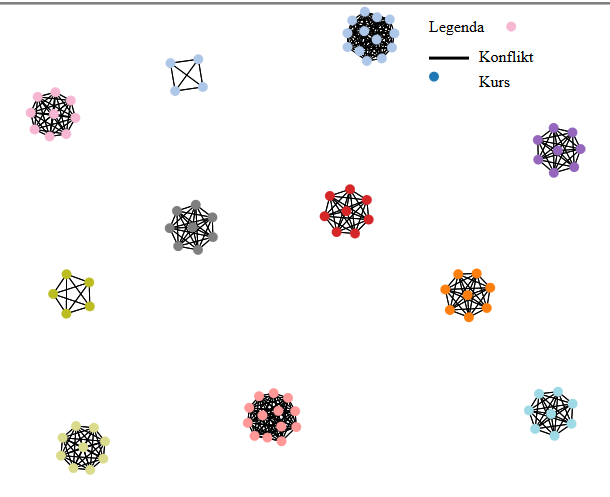
\includegraphics[width=10cm]{szkola1.PNG}
    \caption{Fragment grafu przedstawiający konflikty pomiędzy pomiędzy kursami, uwzględniając zależności związane z tym samym prowadzącym zajęcia. Grafy pełne.}
\end{figure}
\par Graf pokazuje konflikty pomiędzy zajęciami, po uwzględnieniu ograniczeń dotyczących tego samego prowadzącego nauczyciela, który uczy w kilku grupach przedmiotowych. Uzyskana struktura grafu jest prawiłowa, ponieważ w danym czasie nauczyciel jest w stanie prowadzić zajęcia tylko w jednej grupie przedmiotowej. Na wizualizację składają się grafy pełne zawierające wszystkie zależności dotyczące konfliktów uwzględniających tego samego wykładowcę.
\begin{figure}[H]
  \centering
  
   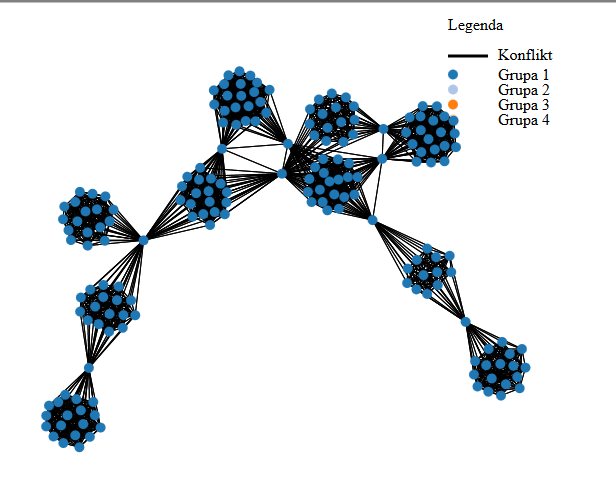
\includegraphics[width=10cm]{fragmentszkola.PNG}
    \caption{Fragment grafu przedstawiający grupy konfliktujących ze sobą kursów ze względu na należenie do tych samych programów nauczania}
\end{figure}
\par Na grafie została pokazana część zależności pomiędzy kursami uwzględniając ograniczenie dotyczące tylko przynależenia kursów do tego samego programu nauczania. Zagnieżdżone grupy kursów reprezentują programy nauczania, zaś wierzchołki łączące te grupy są to zajęcia międzyklasowe.

\subsection{Implementacja}
Projekt został napisany w Python 2.7 \\
Wizualizacje zostały stworzone z wykorzystaniem biblioteki JavaScript D3.js \cite{wiz}
\section{Trudności w analizie i przetwarzaniu danych}
\begin{enumerate}
\item \textbf{Nadmiarowość danych} - po wstępnej analizie okazało się, że część z uzyskanych danych nie jest potrzeba do wyodrębniania istotnych dla algorytmów danych. Uzyskane pliki z danymi zawierające informacje o przedmiotach nauczanych w każdej klasie i nauczycielach prowadzących okazały się być zbędne. W tych danych nie było dołączonej informacji o liczbie godzin realizowanego przedmiotu ani liczbie uczniów uczęszczających na ten przedmiot. 
\item \textbf{Niespójność konwencji nazewnictwa w danych} - utrudniało to w znacznym stopniu analizę danych i powiązań pomiędzy występującymi grupami wchodzącymi w skład klasy. Grupy międzyklasowe mimo tego, że miały dokładnie te same zajęcia w tym samym czasiem i prowadzone były przez tego samego nauczyciela, identyfikatory tych grup były różne dla każdej z klas.
\item \textbf{Niepełne i czasami niepoprawne dane} - brak danych o nauczycielu uczącym danego przedmiotu, brak informacji o liczbie osób uczęszczających na dane zajęcia. Niepełne dane powodowały błędne działanie algorytmu. Uzupełnienie brakujących danych domyślnymi danymi wprowadzało kolejne konflikty pomiędzy kursami, które znacznie utrudniały oraz modyfikowały problem ułożenia planu dla tej szkoły.
\item \textbf{Integracja danych} - konieczność łączenia danych w celu wyodrębnienia informacji o poszczególnych przedmiotach i grupach uczniów. W celu uzyskania danych niezbędnych do specyfikacji problemu koniecznym było połączenie danych z kilku plików, dotyczy to głównie grup międzyklasowych, które występują dla tej szkoły.
\item \textbf{Odtworzenie danych} - konieczność odtworzenia niektórych danych z istniejącego planu zajęć dla szkoły zdefiniowanego pliku ,,Zestawienie planu''. Dane nie zawierały ściśle określonej liczby godzin realizowanego przedmiotu przez daną klasę, dlatego też trzeba było to uzyskać, zliczając poszczególne wystąpienia zajęć w istniejącym planie ułożonym przez szkołę.
\item \textbf{Dostosowanie danych do formatu} - dostosowanie danych szkolnych do formatu zdefiniowanego w danych konkursowych. Narzucony ściśle format danych wejściowych znacznie utrudniał problem przetworzenia danych, gdyż związane było to koniecznością zdefiniowania poszczególnych zajęć, w szczególności zajęć międzyklasowych w zadanej konwencji przez organizatorów konkursu.
\item \textbf{Brakujące dane} - uzupełnienie brakujących danych (typ sali, w jakim typie sali mogą odbywać się zajęcia z danego przedmiotu, wielkość sali).  Dane nie zawierały istotnej informacji o pojemności sali oraz typie sali. Dane te zostały uzupełnione po konsultacji z osobą pracującą w tej szkole i posiadającą wiedzę na ten temat.
\end{enumerate}




\chapter{Testy i porównanie algorytmów}
\section{Analiza działania poszczególnych algorytmów}
\subsection{Algorytm Roju Cząsteczek}
\subsubsection{Problemy związane z rozwiązaniem}
\par Podczas analizy oraz testowania zaimplementowanego rozwiązania, okazało się, że algorytm jest mało skuteczny, gdyż nie był w stanie usunąć całkowicie naruszeń ograniczeń twardych. Ograniczenia te w bezpośredni sposób wpływają na prawidłowość wygenerowanego planu zajęć.
\par W związku z tym zdecydowałem się na wprowadzenie dodatkowej kary: do kary za ograniczenia miękkie dodaję za każde naruszenie ograniczenia twardego 1 milion punktów kary. Dzięki temu, algorytm w pierwszej kolejności bierze pod uwagę ograniczenia twarde, próbując je wyeliminować, a potem dopiero ograniczenia miękkie. \\

Poniższy wykres pokazuje efektywność algorytmu. Uwagę należy zwrócić na skalę przyjętą na osi y. Wartości nie schodzą poniżej $10^{7}$ czyli wynik w najlepszym wypadku nadal łamie 10 twardych ograniczeń.

\begin{figure}[H]
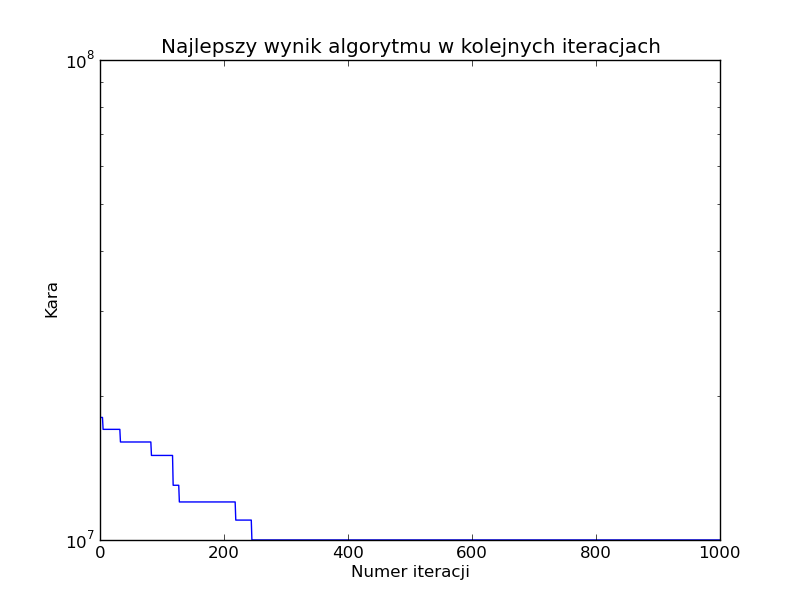
\includegraphics[width=10cm]{img/standard_penalty.png}
\centering
\end{figure}
\par W celu sprawdzenia przyczyny tego zachowania przyjrzałem się zachowaniu pojedynczej cząsteczki. Okazało się, że kara za kolejno generowane plany oscyluje wokół kary wyliczonej dla początkowego planu, co potwierdza poniższy wykres.  
\begin{figure}[H]
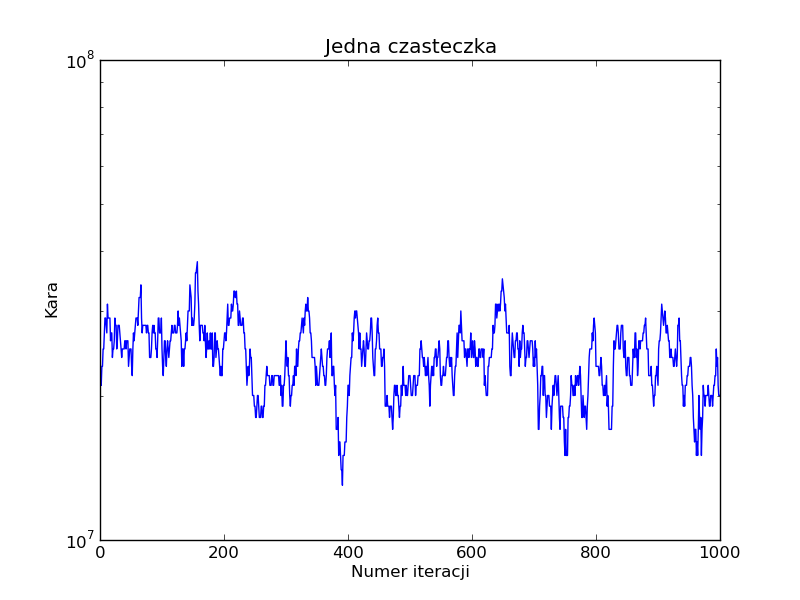
\includegraphics[width=10cm]{img/standard_particle.png}
\centering
\end{figure}
\par Na podstawie dalszej analizy okazało się, że wszystkie cząsteczki zachowują się bardzo podobnie, co można zaobserwować na wykresie. 
\begin{figure}[H]
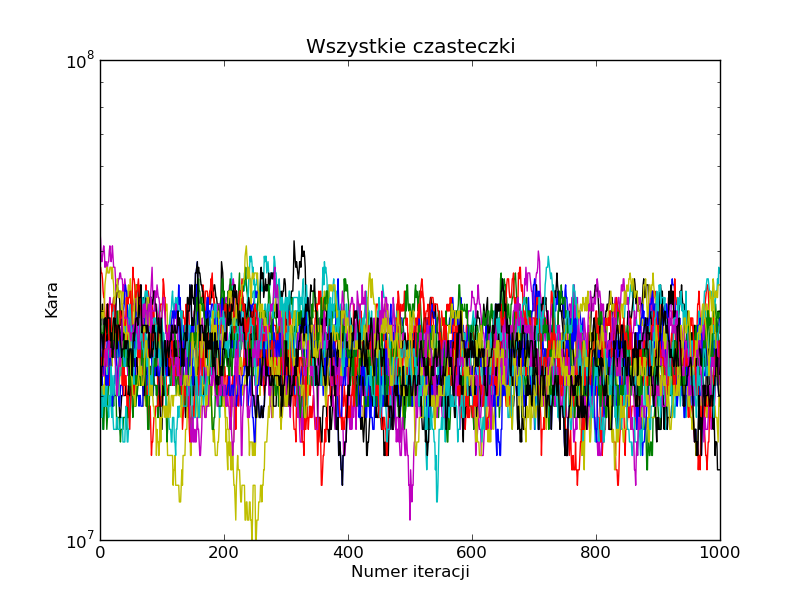
\includegraphics[width=10cm]{img/standard_particle_all.png}
\centering
\end{figure}
\subsubsection{Modyfikacje}
\par W celu dojścia do lepszego rozwiązania problemu układania planu zajęć za pomocą algorytmu PSO, rozważyłem dwie modyfikacje zaproponowanego wcześniej algorytmu.Pierwsza z nich to  ,,podążanie za lokalnie najlepszym planem'', a druga zaś ,,podążanie za globalnie najlepszym planem''. Obie modyfikacje są analogiczne do siebie, jedyną ich różnicą jest tylko plan, który jest brany pod uwagę. Dokonałem również modyfikacji fazy dotyczącej oceny aktualnego rozwiązania, która jest przeprowadzana na początku każdej iteracji. Ponadto został dodany warunek, że jeśli aktualny plan jest gorszy od najlepszego planu to zostaje on zamieniony na najlepszy plan. Zrezygnowałem również z realizacji krotów 3 i 4, opisanych w algorytmie PSO.

\par W przypadku gdy każda cząsteczka ,,podąża za swoim lokalnie najlepszym planem'' istnieje mniejsze ryzyko, że algorytm pozostanie w lokalnym minimum przestrzeni rozwiązań. Natomiast podczas ,,podążania za globalnie najlepszym planem'' algorytm będzie znacznie szybciej dążył do najbliższego minimum.

\par Opcja ,,podążania za lokalnie najlepszym planem'' okazała się być dużo efektywniejsza od podstawowego algorytmu. W tym przypadku twarde ograniczenia nie były naruszone, co potwierdza poniższy wykres.
\begin{figure}[H]
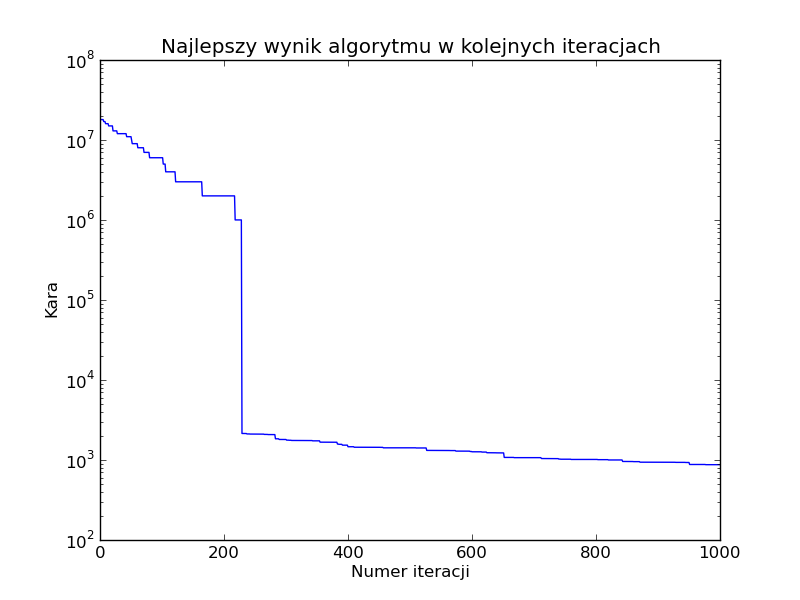
\includegraphics[width=10cm]{img/localbest_penalty.png}
\centering
\end{figure}
\par Analizując pojedynczą cząsteczkę można zauważyć, że kara często zmienia się od małych wartości do wartości powyżej miliona. Spowodowane jest to tym, że po zamianie dwóch lekcji w poprzedniej iteracji pojawił się konflikt z twardymi ograniczeniami. W tej sytuacji algorytm powraca do poprzedniego rozwiązania. Na poniższych wykresach widać zachowanie dla pojedynczej cząsteczki oraz dla wszystkich cząsteczek.
\begin{figure}[H]
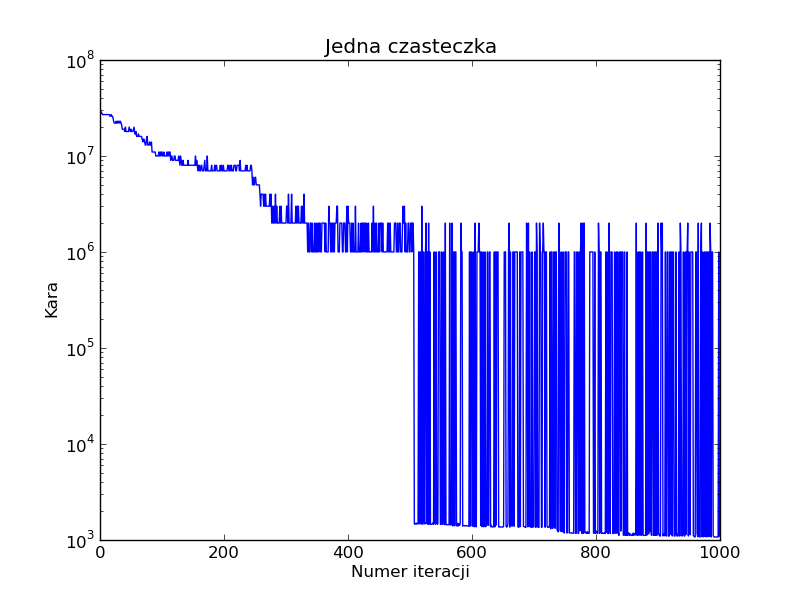
\includegraphics[width=10cm]{img/localbest_particle.png}
\centering
\end{figure}
\begin{figure}[H]
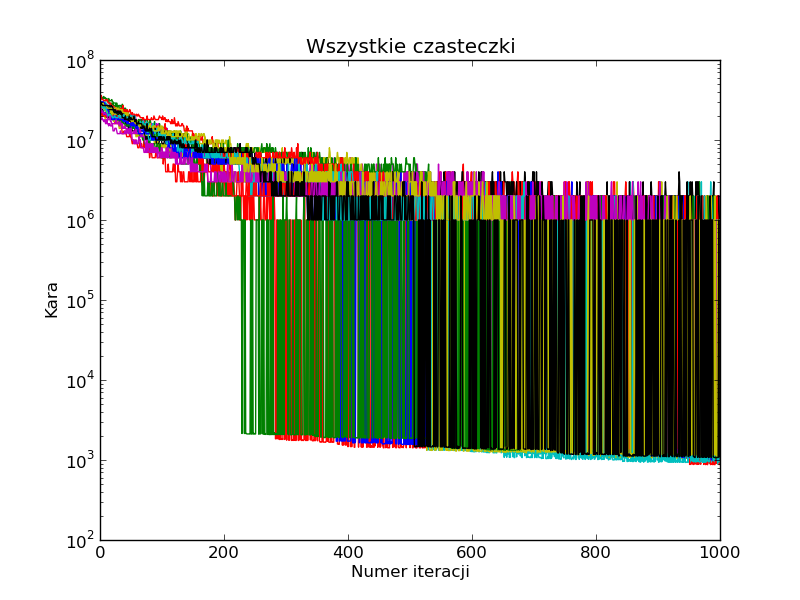
\includegraphics[width=10cm]{img/localbest_particle_all.png}
\centering
\end{figure}
\par Opcja podążania za globalnie najlepszym planem okazała się być bardziej efektywna. Sporym zaskoczeniem był brak problemów z lokalnymi minimami przestrzeni rozwiązań. Poniższy wykres pokazuje skuteczność modyfikacji.
\begin{figure}[H]
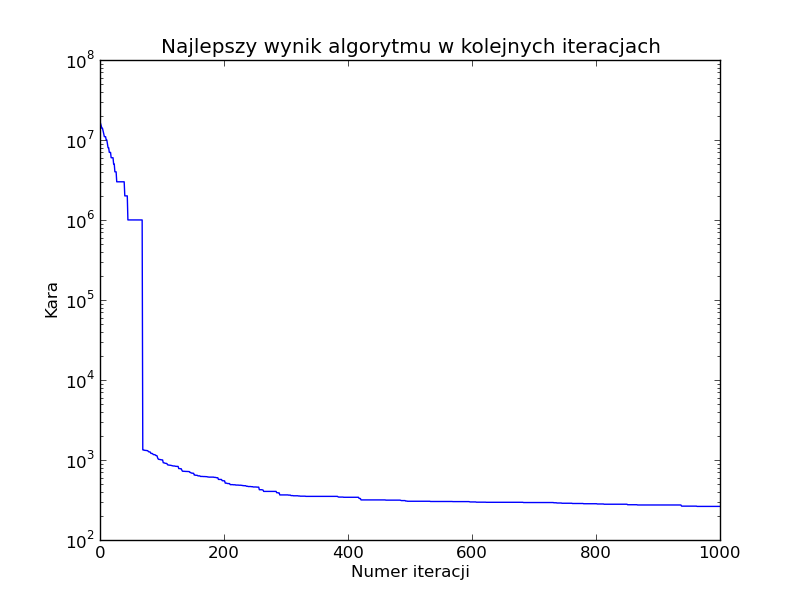
\includegraphics[width=10cm]{img/globalbest_penalty.png}
\centering
\end{figure}
\par W tym przypadku cząsteczki zachowywały się bardzo podobnie. Jedyną różnicą była prędkość z jaką malała funkcja kary, można to zauważyć na poniższych wykresach. 

\begin{figure}[H]
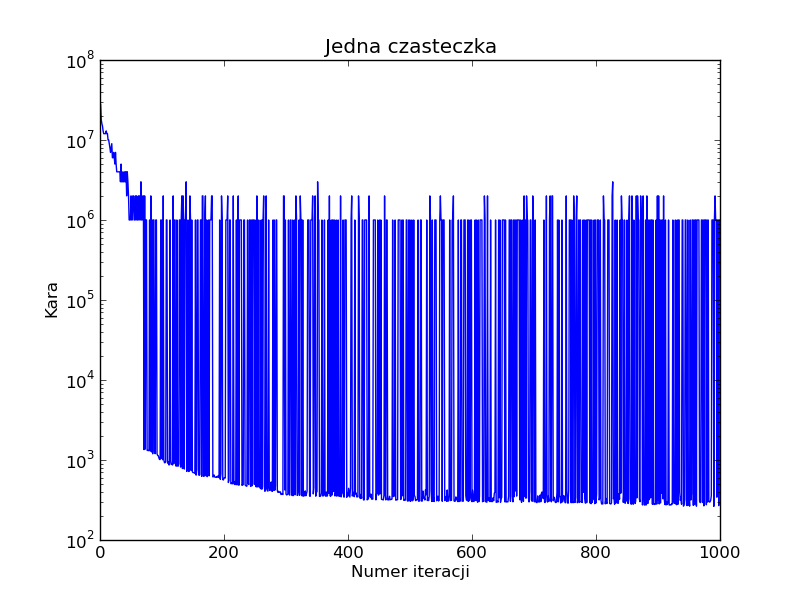
\includegraphics[width=10cm]{img/globalbest_particle.png}
\centering
\end{figure}

\begin{figure}[H]
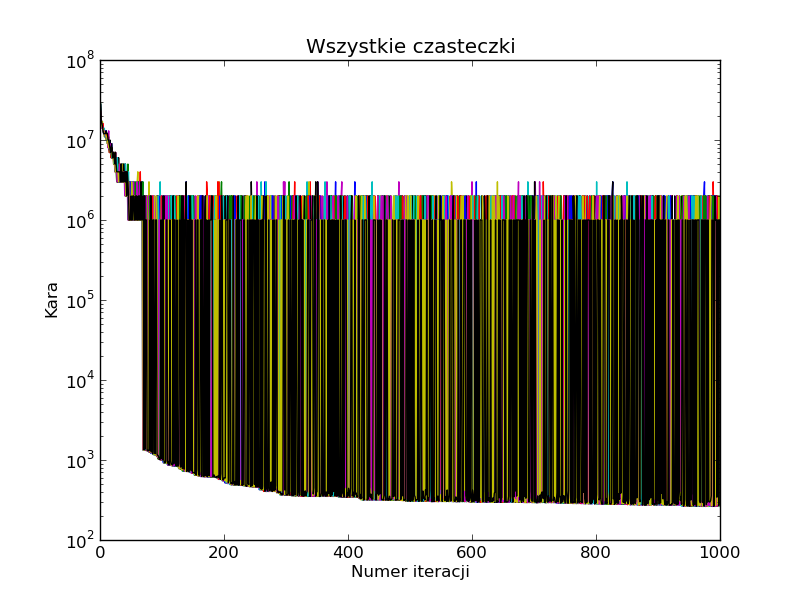
\includegraphics[width=10cm]{img/globalbest_particle_all.png}
\centering
\end{figure}

\subsubsection{Ostateczne rozwiązanie}

-\par Jako ostateczne rozwiązanie wybrałem podążanie za globalnie najlepszym planem. Jest to spowodowane tym, że mimo wielu testów nie udało mi się znaleźć przypadku kiedy podążanie za lokalnie najlepszym planem wypadłoby lepiej. 
\subsection{Algorytm Adaptacyjny Tabu}
Przedstawienie działania algorytmu dla wybranych testów.
\par \textbf{Test 1}
\begin{figure}[H]
  \caption{Wykres zależności funkcji oceny od czasu}
  \centering
    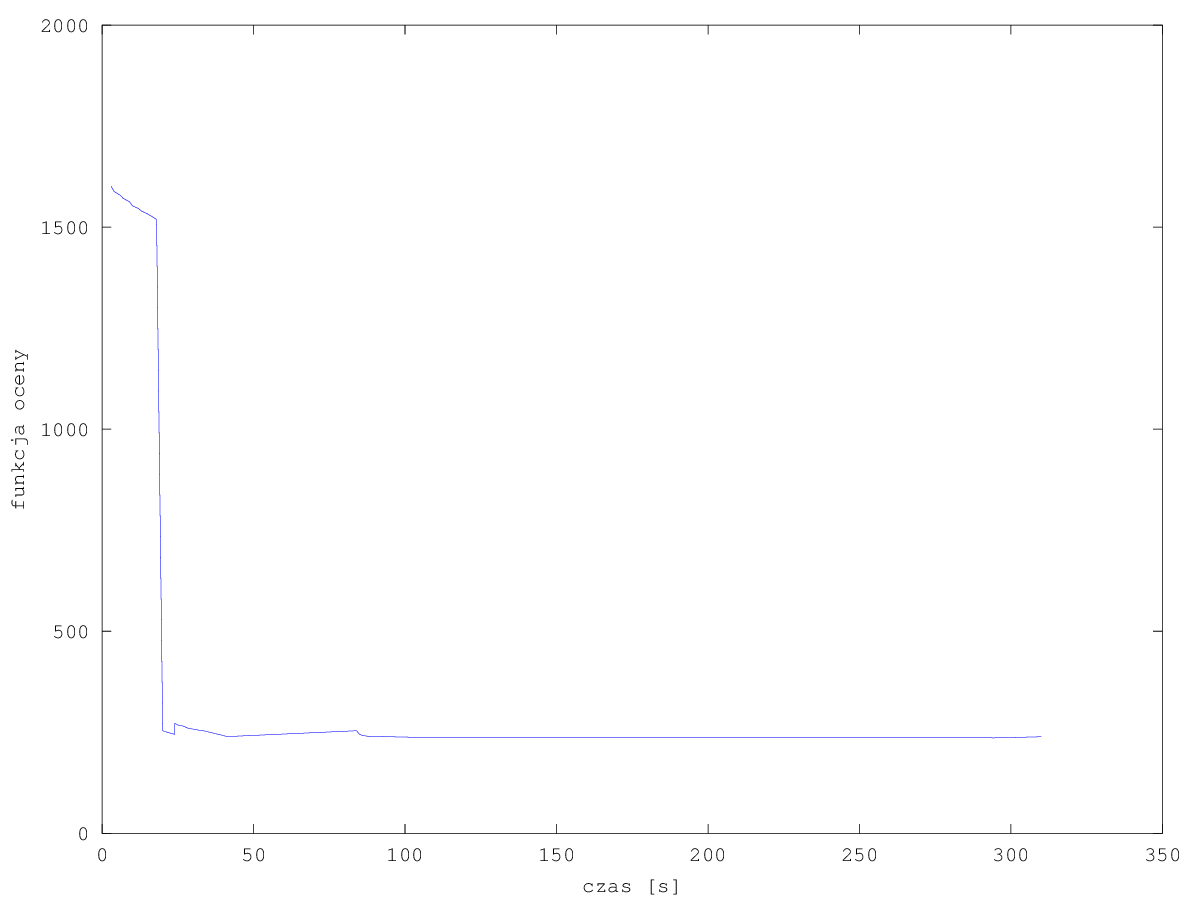
\includegraphics[width=10cm]{ogolny.png}
\end{figure}
\begin{figure}[H]
  \caption{Wykres zależności funkcji oceny od czasu, bez uwzględnienia fazy inicjalizacji}
  \centering
    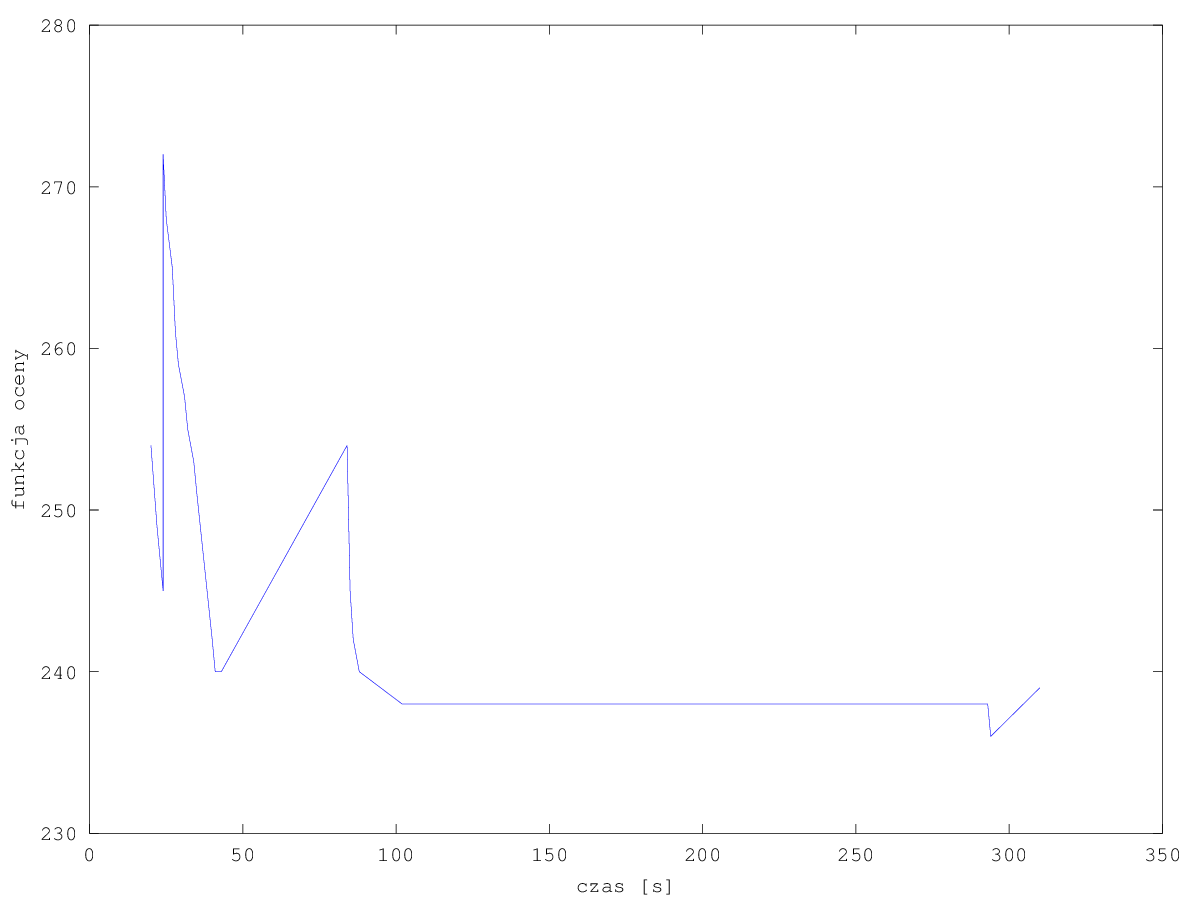
\includegraphics[width=10cm]{szczeg.png}
\end{figure}
\par \textbf{Test 2}
\begin{figure}[H]
  \caption{Wykres zależności funkcji oceny od czasu}
  \centering
    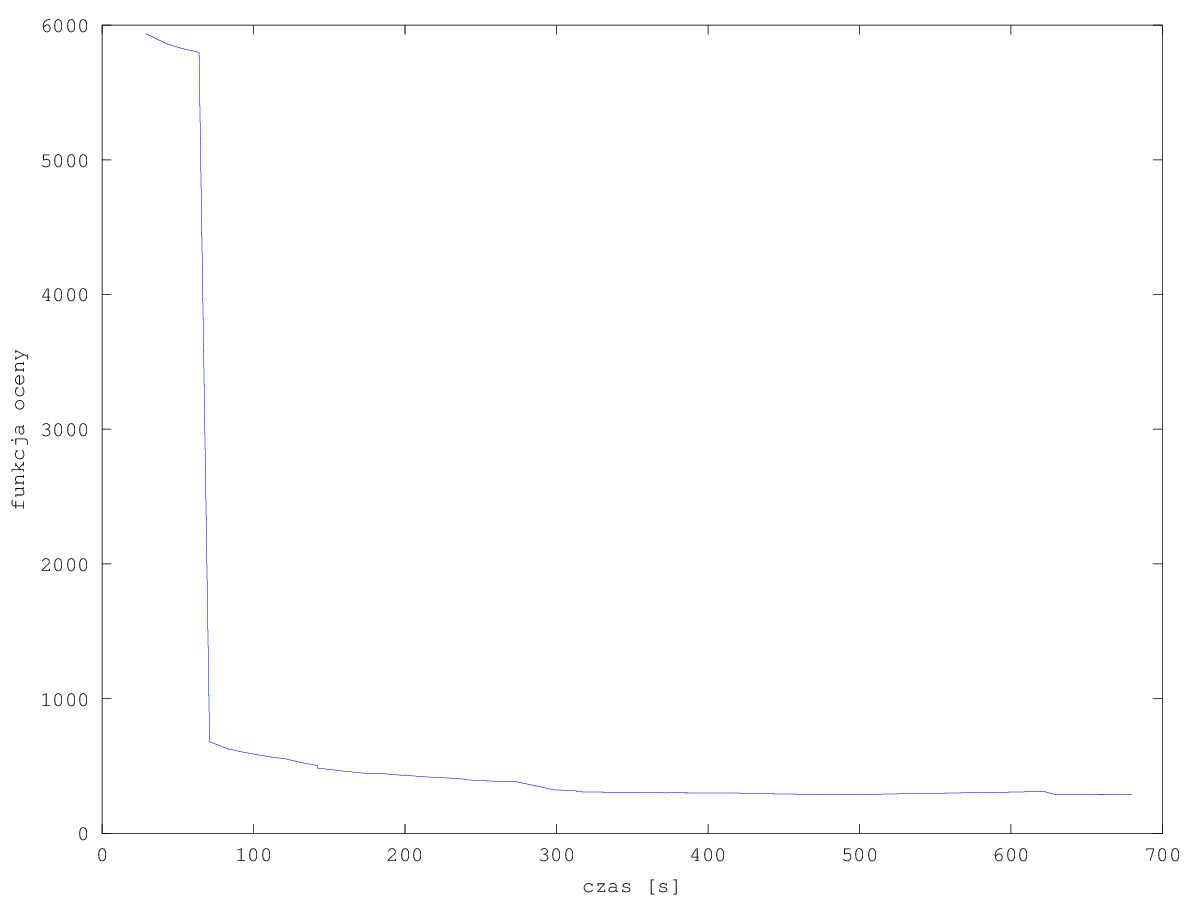
\includegraphics[width=10cm]{ogolny2_instancja.png}
\end{figure}
\begin{figure}[H]
  \caption{Wykres zależności funkcji oceny od czasu, bez uwzględnienia fazy inicjalizacji}
  \centering
    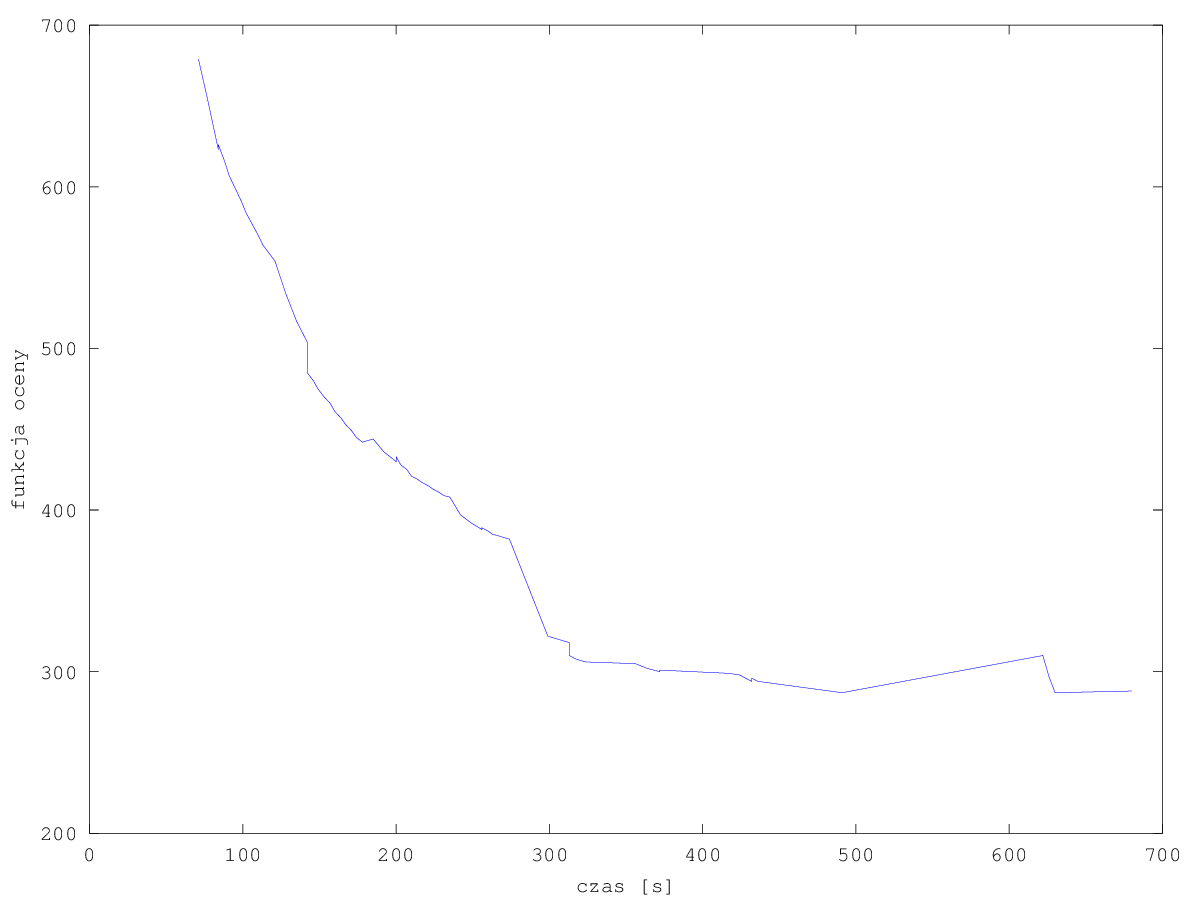
\includegraphics[width=10cm]{szczegolowy2_instancja.png}
\end{figure}
\subsection{Algorytm Genetyczny}
\section{Specyfikacja testów}
Dane testowe pobrane zostały z konkursu ,,International Timetabling Competition 2007''. Do oceny rozwiązań używany jest oryginalny walidator rozwiązań, zapewniony przez organizatorów konkursu.
\subsection{Test 1}
\begin{table}[H]
\begin{center}
 
\begin{tabular}{ |l|l| }
\hline
$Liczba\ kursów$ & $30$\\
\hline
$Liczba\ programów\ nauczania$ & $14$\\
\hline
$Liczba\ dni$ & $5$ \\
\hline
$Licza\ przedziałów\ czasowych$ & $6$ \\
\hline
$Liczba\ ograniczeń$ & $53$ \\
\hline
$Liczba\ sal$ & $6$ \\
\hline
\end{tabular}
\end{center}
\end{table}
\par Wyniki działania algorytmów- ocena wygenerowanych planów zajęć: \\
Parametry dla algorytmów:
\begin{enumerate}
\item GA - liczba osobników: 100, liczba iteracji: 500, szacowany czas działania algorytmu: 150 s
\item PSO - liczba cząsteczek: 20, liczba iteracji 10000, szacowany czas działania algorytmu: 40 min
\item ATS - czas działania: 120 s
\end{enumerate}
\begin{table}[H]
\begin{center}

\begin{tabular}{ |l|l|l|l| }
\hline
 & $GA$ & $PSO$ & $ATS$\\
\hline
${H}_{1}\ Wykłady$ & $0$ & $0$ & $0$\\
\hline
$H_{2}\ Zajętość\ sali$ & $0$ & $0$ & $0$\\
\hline
$H_{3}\ Konflikty\ pomiędzy\ kursami$ & $0$ & $0$ & $0$ \\
\hline
$H_{4}\ Dostępność\ wykładowcy$ & $0$ & $0$ & $0$ \\
\hline
$S_{1}\ Wielkość\ sali$ & $4$ & $5$ & $205$ \\
\hline
$S_{2}\ Stabilność\ pomieszczenia$ & $14$ & $24$ & $32$ \\
\hline
$S_{3}\ Minimalna\ liczba\ dni$ & $0$ & $0$ & $0$ \\
\hline
$S_{4}\ Zwartość\ zajęć$ & $56$ & $8$ & $6$ \\
\hline
$Funkcja\ oceny$ & $74$ & $37$ & $243$ \\
\hline
\end{tabular}
\end{center}
\caption {Wyniki uzyskane przez poszczególne algorytm}
\end{table}

\par  Wykresy zmiany funkcji oceny w zależności od liczby odwołań do funkcji oceny dla poszczególnych algorytmów.
\begin{figure}[H]
  \caption{Algorytm Genetyczny}
  \centering
    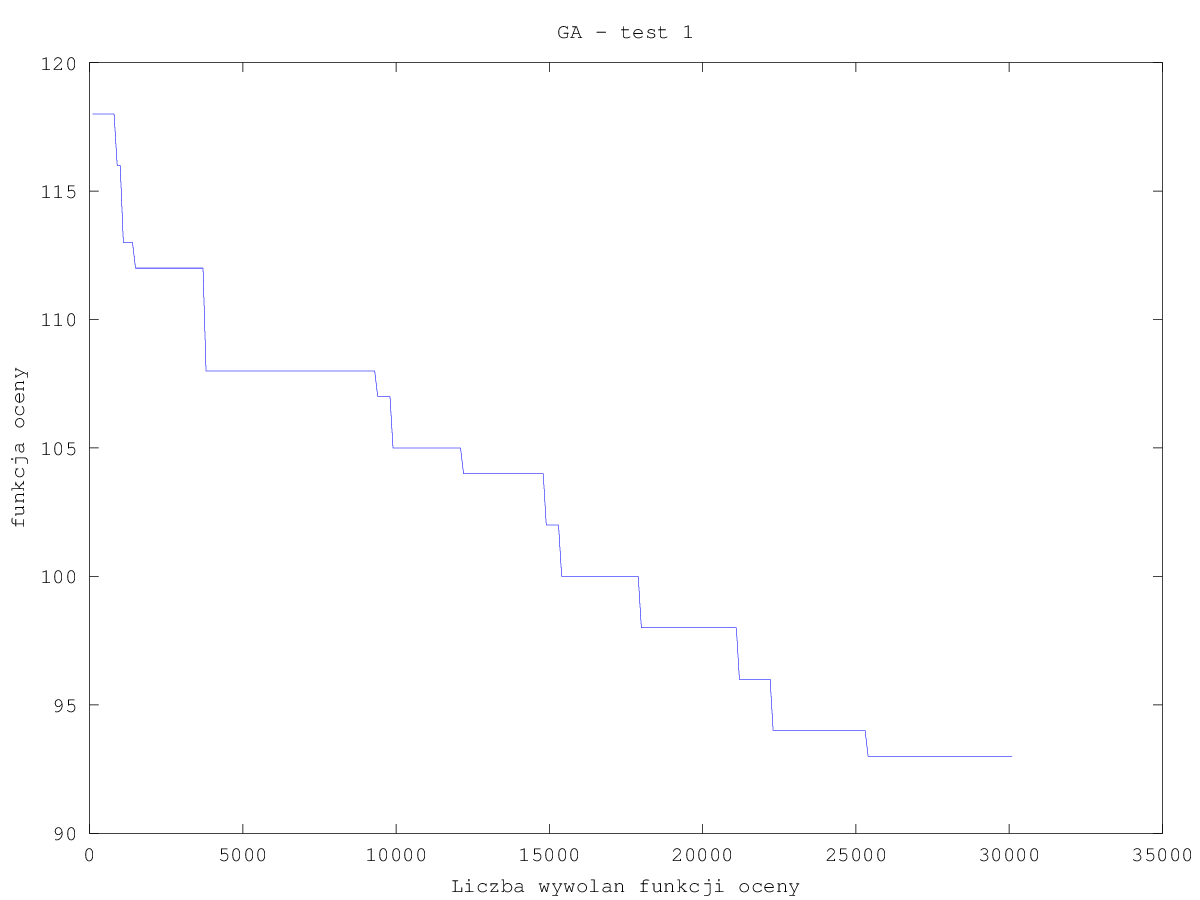
\includegraphics[width=10cm]{ga_test_1.png}
\end{figure}
\begin{figure}[H]
  \caption{Algorytm Roju Cząsteczek}
  \centering
    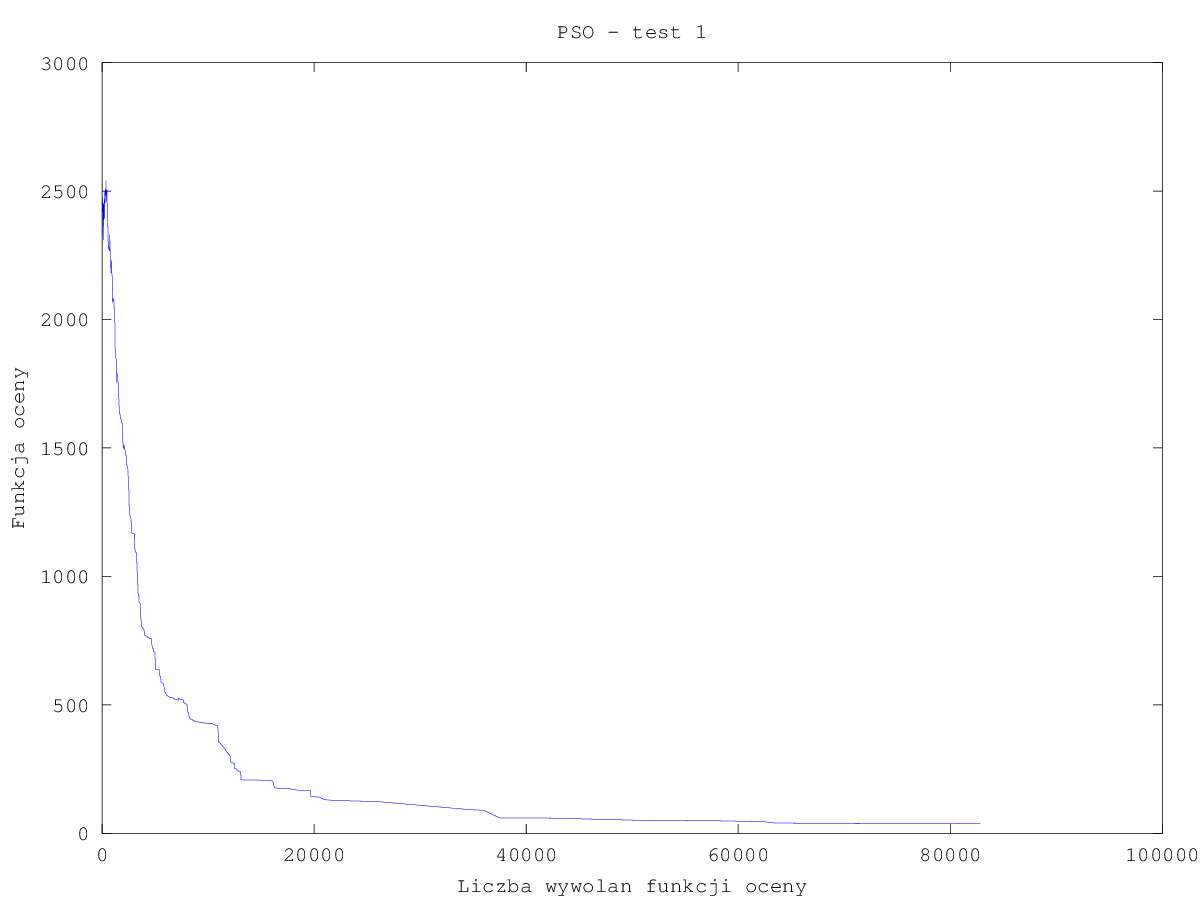
\includegraphics[width=10cm]{pso_1.png}
\end{figure}
\begin{figure}[H]
  \caption{Algorytm Adaptacyjny Tabu}
  \centering
    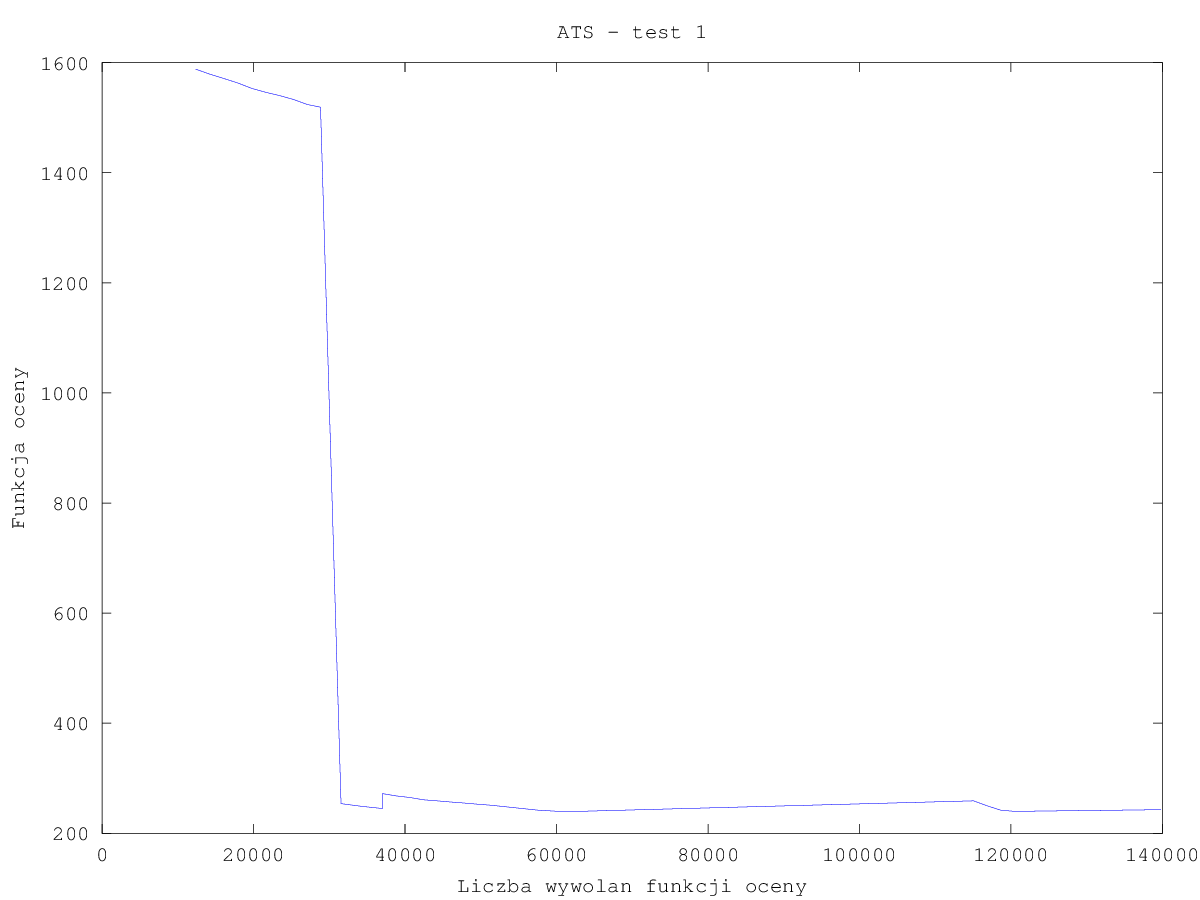
\includegraphics[width=10cm]{ats_test_1.png}
\end{figure}

\subsubsection{Test 1 - wizualizacja}
\begin{figure}[H]
  \caption{Graf przedstawiający wszystkie zależności pomiędzy kursami (uwzględniając tych samych prowadzących nauczycieli oraz należenie kursu do tego samego programu nauczania) }
  \centering
    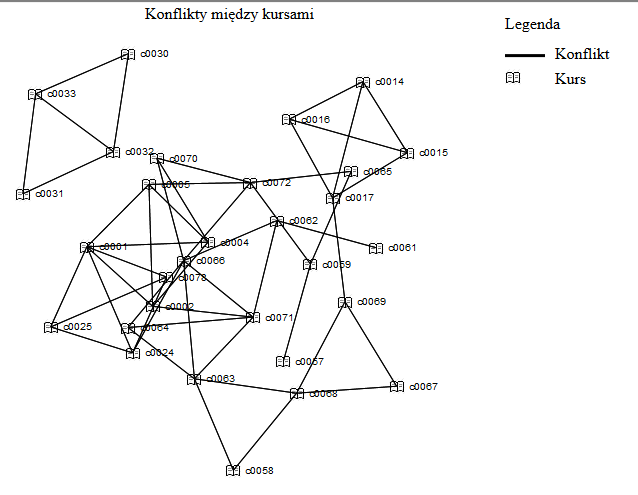
\includegraphics[width=0.8\textwidth]{test1.PNG}
\end{figure}


\begin{figure}[H]
  \caption{Graf uwzględniający zależności pomiędzy kursami uwzględniając prowadzących dane kursy}
  \centering
    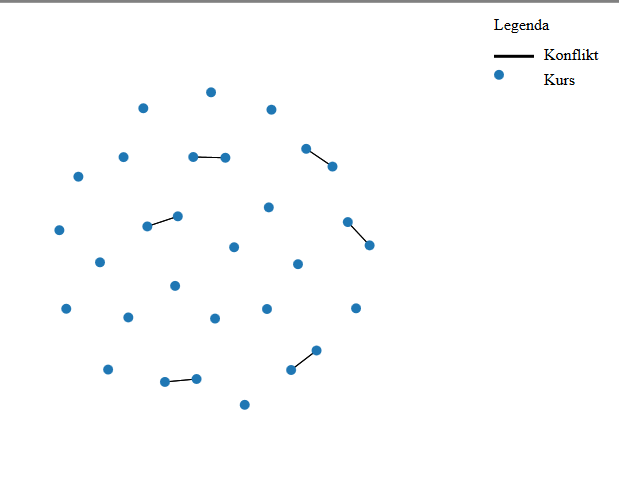
\includegraphics[width=0.8\textwidth]{test1_teach.PNG}
\end{figure}
\begin{figure}[H]
  \caption{Graf uwględniający grupy zależnych od siebie kursów wchodzących w skład tego samego programu nauczania}
  \centering
    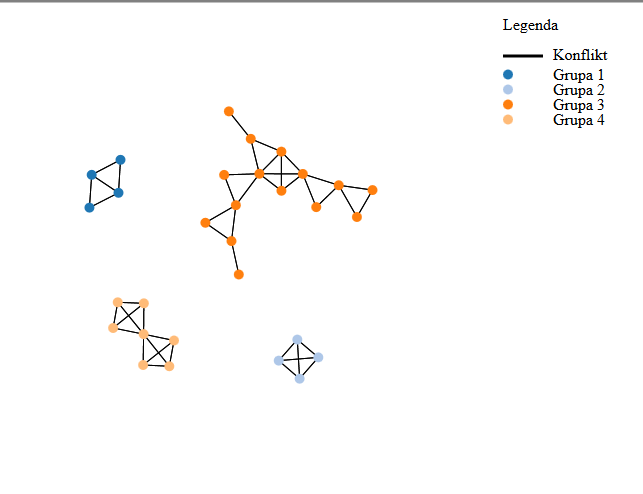
\includegraphics[width=0.8\textwidth]{test1_con.PNG}
\end{figure}
\subsection{Test 2}
\begin{table}[H]
\begin{center}

\begin{tabular}{ |c|c|c|c| }
\multicolumn{1}{r}{}
 &  \multicolumn{1}{c}{$$}
 & \multicolumn{1}{c}{$$} 
 \\
\cline{1-2}
$Liczba\ kursów$ & $82$\\
\cline{1-2}
$Liczba\ programów\ nauczania$ & $70$\\
\cline{1-2}
$Liczba\ dni$ & $5$ \\
\cline{1-2}
$Licza\ przedziałów\ czasowych$ & $5$ \\
\cline{1-2}
$Liczba\ ograniczeń$ & $513$ \\
\cline{1-2}
$Liczba\ sal$ & $16$ \\
\cline{1-2}
\end{tabular}
\end{center}
\caption {Specyfikacja danych - Test 2}
\end{table}
\par Wyniki działania algorytmów- ocena wygenerowanych planów zajęć: \\
Parametry dla algorytmów:
\begin{enumerate}
\item GA - liczba osobników: 200, liczba iteracji: 1000, szacowany czas działania algorytmu: 33 min
\item PSO - liczba cząsteczek: 20, liczba iteracji 10000, szacowany czas działania algorytmu: 180 min
\item ATS - czas działania: 480 s
\end{enumerate}
\begin{table}[H]
\begin{center}

\begin{tabular}{ |l|l|l|l| }
\hline
 & $GA$ & $PSO$ & $ATS$\\
\hline
${H}_{1}\ Wykłady$ & $0$ & $1$ & $0$\\
\hline
$H_{2}\ Zajętość\ sali$ & $0$ & $0$ & $0$\\
\hline
$H_{3}\ Konflikty\ pomiędzy\ kursami$ & $0$ & $0$ & $0$ \\
\hline
$H_{4}\ Dostępność\ wykładowcy$ & $0$ & $2$ & $0$ \\
\hline
$S_{1}\ Wielkość\ sali$ & $119$ & $54$ & $0$ \\
\hline
$S_{2}\ Stabilność\ pomieszczenia$ & $63$ & $51$ & $143$ \\
\hline
$S_{3}\ Minimalna\ liczba\ dni$ & $70$ & $74$ & $40$ \\
\hline
$S_{4}\ Zwartość\ zajęć$ & $424$ & $150$ & $104$ \\
\hline
$Funkcja\ oceny$ & $676$ & $330$ & $287$ \\
\hline
\end{tabular}
\end{center}
\caption {Wyniki uzyskane przez poszczególne algorytmy}
\end{table}

\par  Wykresy zmiany funkcji oceny w zależności od liczby odwołań do funkcji oceny dla poszczególnych algorytmów.
\begin{figure}[H]
  \caption{Algorytm Genetyczny}
  \centering
    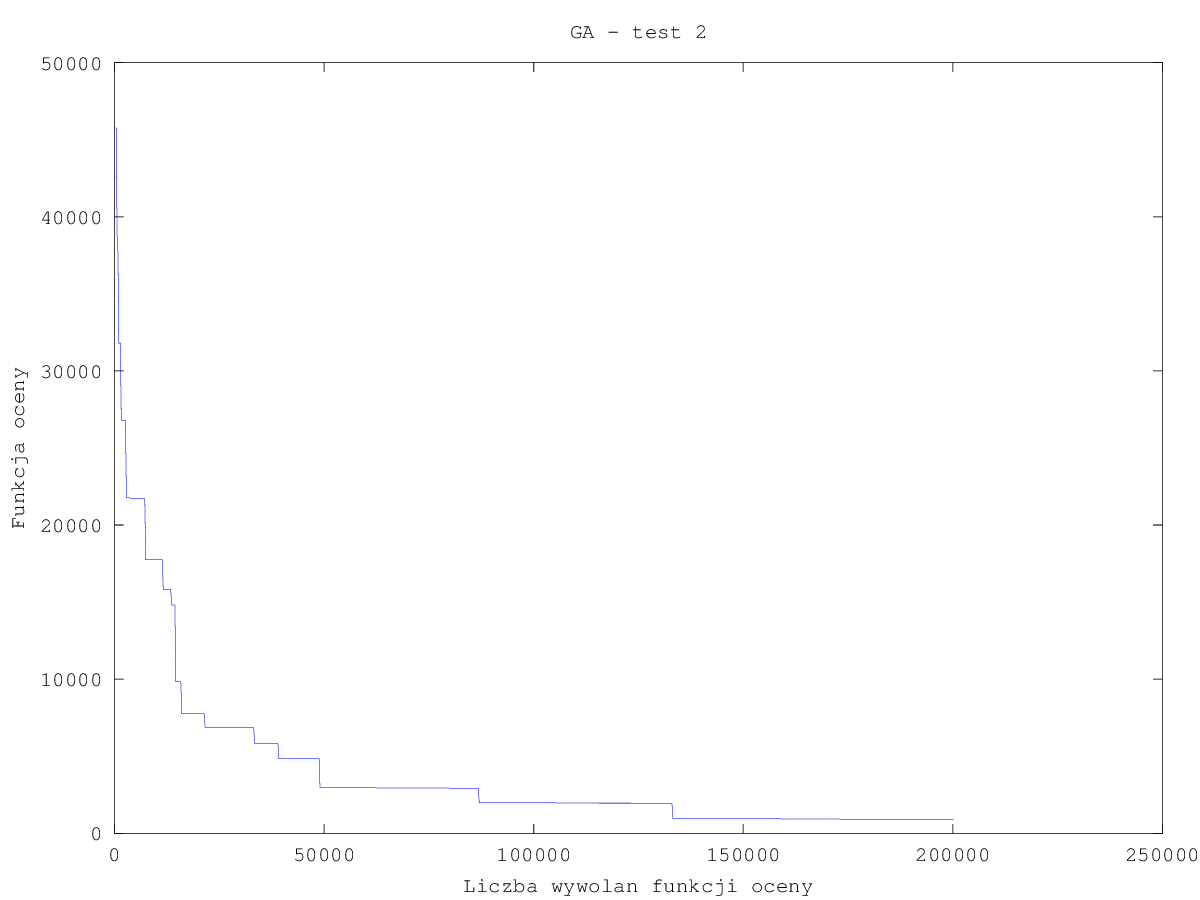
\includegraphics[width=10cm]{ga_test_2.png}
\end{figure}
\begin{figure}[H]
  \caption{Algorytm Roju Cząsteczek}
  \centering
    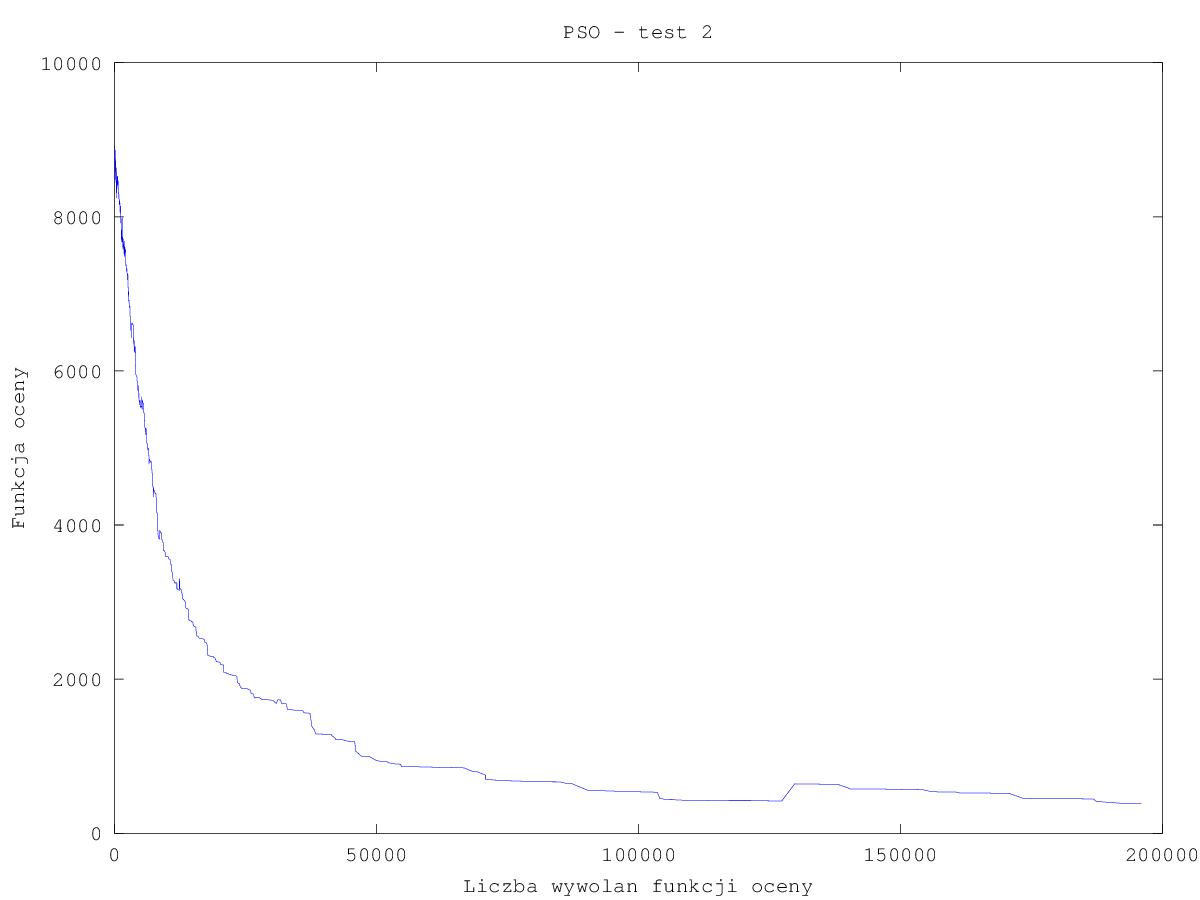
\includegraphics[width=10cm]{pso_2.png}
\end{figure}
\begin{figure}[H]
  \caption{Algorytm Adaptacyjny Tabu}
  \centering
    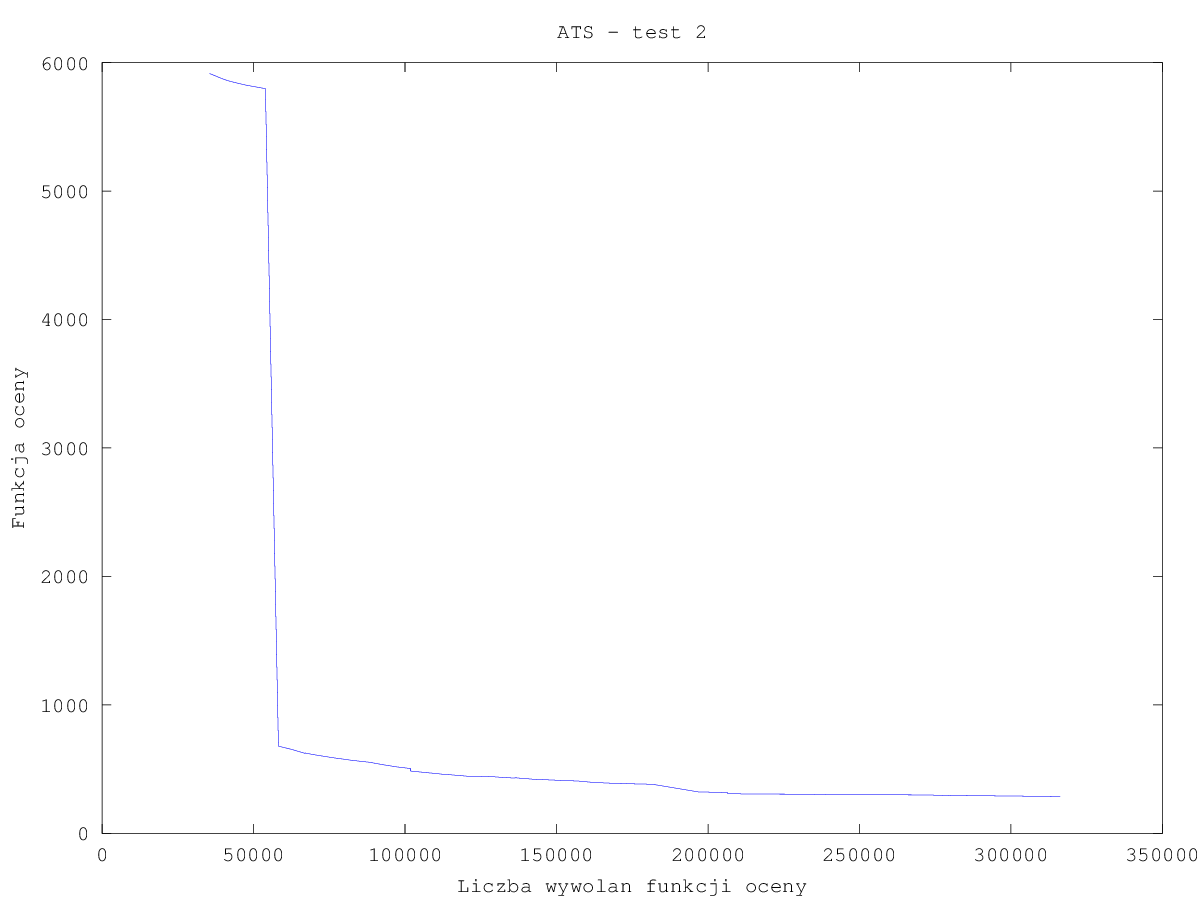
\includegraphics[width=10cm]{ats_test_2.png}
\end{figure}
\subsection{Test 3}
\begin{table}[H]
\begin{center}

\begin{tabular}{ |c|c|c|c| }
\multicolumn{1}{r}{}
 &  \multicolumn{1}{c}{$$}
 & \multicolumn{1}{c}{$$} 
 \\
\cline{1-2}
$Liczba\ kursów$ & $72$\\
\cline{1-2}
$Liczba\ programów\ nauczania$ & $68$\\
\cline{1-2}
$Liczba\ dni$ & $5$ \\
\cline{1-2}
$Licza\ przedziałów\ czasowych$ & $5$ \\
\cline{1-2}
$Liczba\ ograniczeń$ & $382$ \\
\cline{1-2}
$Liczba\ sal$ & $16$ \\
\cline{1-2}
\end{tabular}
\end{center}
\caption {Specyfikacja danych - Test 3}
\end{table}
\par Wyniki działania algorytmów- ocena wygenerowanych planów zajęć: \\
Parametry dla algorytmów:
\begin{enumerate}
\item GA - liczba osobników: 200, liczba iteracji: 1000, szacowany czas działania algorytmu: 33 min
\item PSO - liczba cząsteczek: 20, liczba iteracji 5000, szacowany czas działania algorytmu: 90 min
\item ATS - czas działania: 16min
\end{enumerate}
\begin{table}[H]
\begin{center}

\begin{tabular}{ |l|l|l|l| }
\hline
 & $GA$ & $PSO$ & $ATS$\\
\hline
${H}_{1}\ Wykłady$ & $0$ & $0$ & $0$\\
\hline
$H_{2}\ Zajętość\ sali$ & $0$ & $0$ & $0$\\
\hline
$H_{3}\ Konflikty\ pomiędzy\ kursami$ & $0$ & $0$ & $0$ \\
\hline
$H_{4}\ Dostępność\ wykładowcy$ & $0$ & $1$ & $0$ \\
\hline
$S_{1}\ Wielkość\ sali$ & $82$ & $109$ & $12$ \\
\hline
$S_{2}\ Stabilność\ pomieszczenia$ & $50$ & $57$ & $125$ \\
\hline
$S_{3}\ Minimalna\ liczba\ dni$ & $20$ & $70$ & $40$ \\
\hline
$S_{4}\ Zwartość\ zajęć$ & $412$ & $202$ & $102$ \\
\hline
$Funkcja\ oceny$ & $564$ & $438$ & $279$ \\
\hline
\end{tabular}
\end{center}
\caption {Wyniki uzyskane przez poszczególne algorytmy}
\end{table}
\par  Wykresy zmiany funkcji oceny w zależności od liczby odwołań do funkcji oceny dla poszczególnych algorytmów.
\begin{figure}[H]
  \caption{Algorytm Genetyczny}
  \centering
    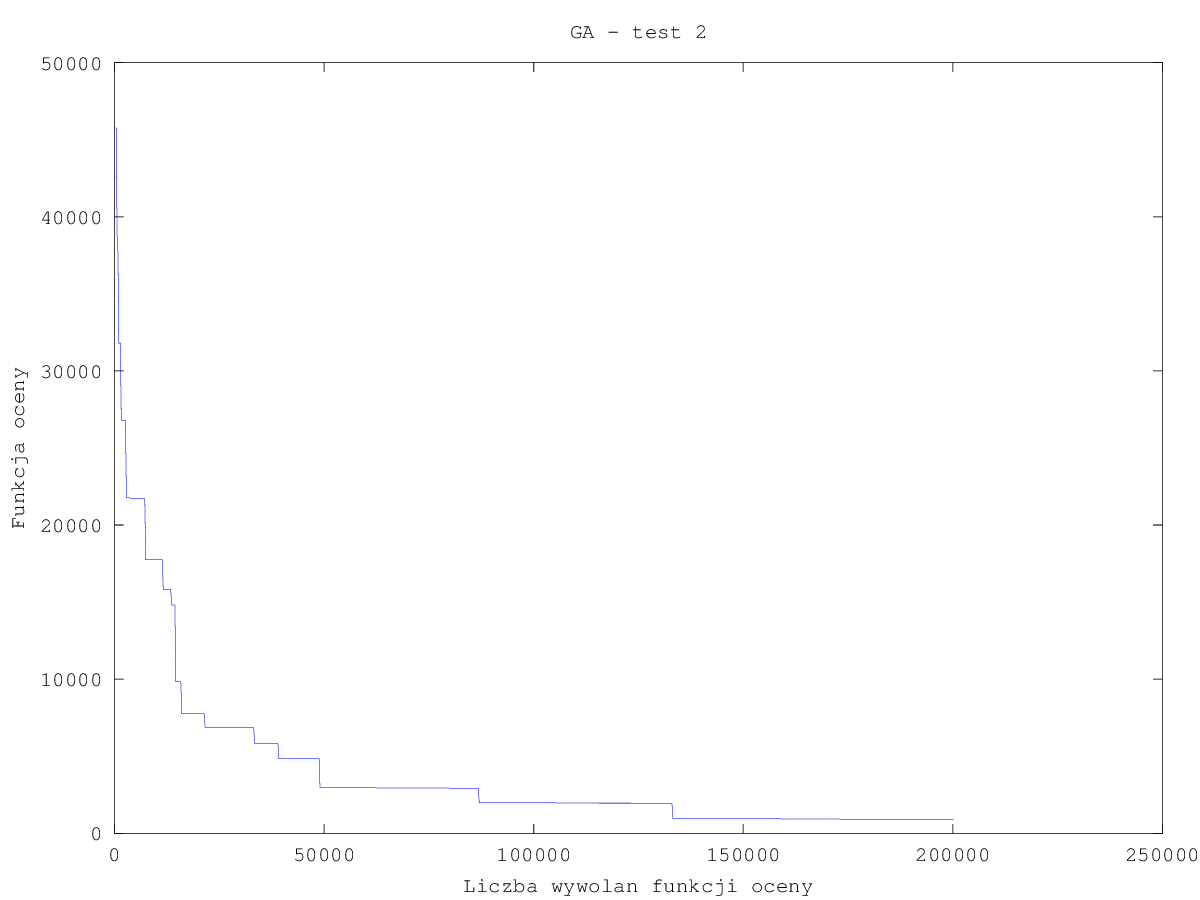
\includegraphics[width=10cm]{ga_test_2.png}
\end{figure}
\begin{figure}[H]
  \caption{Algorytm Roju Cząsteczek}
  \centering
    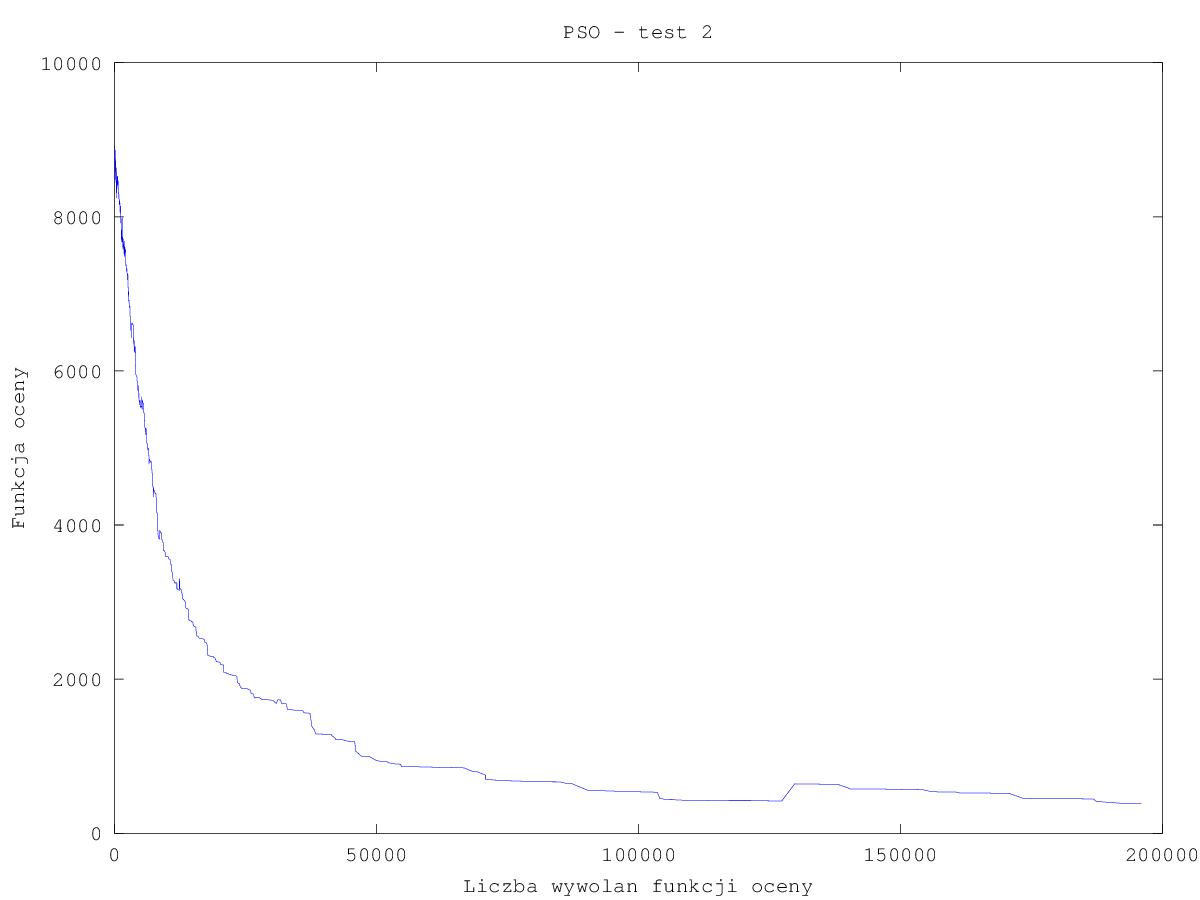
\includegraphics[width=10cm]{pso_2.png}
\end{figure}
\begin{figure}[H]
  \caption{Algorytm Adaptacyjny Tabu}
  \centering
    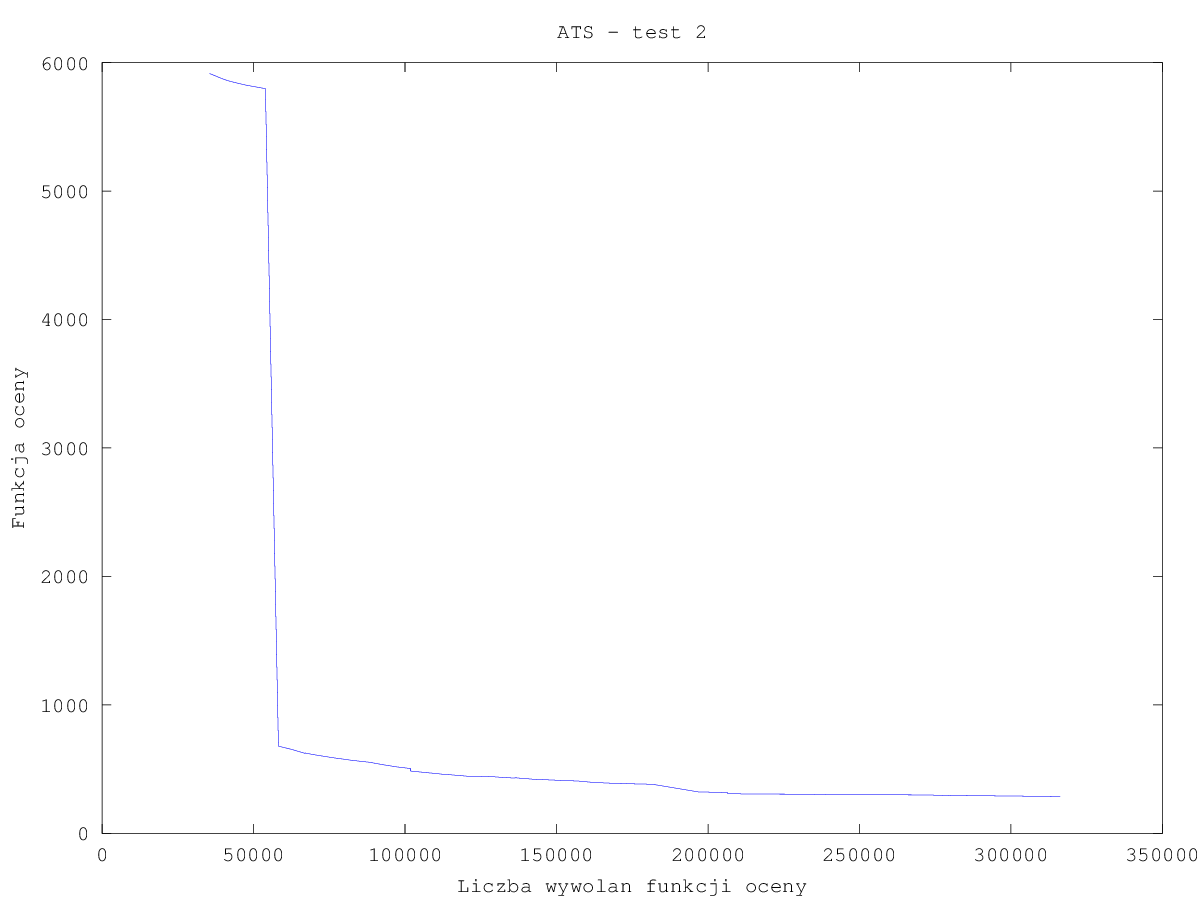
\includegraphics[width=10cm]{ats_test_2.png}
\end{figure}

\par PSO nie usuwan hardów (wybrana metoda nie odporna na lokane minima), . Ostateczne rozw jest najprostsze - to slabo dziala
\par badawczo 
GA - niepewne rozw element losow (roznie generuje poczatkowe rozwiazania), duza liczba osobnikow, upodobniaja zwiekszenie wspolczynnika mutacji do wyjscia z lokalnego minimum
\par system prosty do wykorzystania alg, otwarty na rozbudowe: rezcna edycja planu, wprowadzenie przez nuczycieli 









\chapter{Sposób użytkowania systemu}

\chapter{Podsumowanie}
\paragraph{}
\par Realizacja projektu inżynierskiego postawiła nas przed ciekawą możliwością głębszego zapoznania się z problemem układania planów zajęć, zagłębienia się w literaturę tematu oraz implementację wybranych przez nas algorytmów: Algorytmu Genetycznego, Algorytmu Adaptacyjnego Tabu oraz Algorytmu Roju Cząsteczek. Zagadnienie naszej pracy inżynierskiej poszerzyliśmy o te dwa dodatkowe algorytmy, dzięki którym mogliśmy porównać działanie Algorytmu Genetycznego w stosunku do innych podejść również nakierowanych na znalezienie opytmalnego, wykonywalnego planu zajęć
\par Pierwotną, planowaną wizją było przystosowanie zaimplementowanych algorytmów do systemu Politechniki Gdańskiej moja.pg. Niestety mimo licznych trudności związanych z prawem dotyczącym ochrony danych osobowych nie udało się uzyskać niezbędnych danych do realizacji projektu. W konsekwencji zdecydowaliśmy się na przystosowanie naszych algorytmów do danych uzyskanych z jednej ze szkół ponadgimnazjalnej, w celu urealnienia tego problemu. Większość wstępnych założeń dotycząca implementacji algorytmów została zrealizowana, a uzyskane przez nas wyniki potwierdziły nasze przypuszczenia co do skuteczności poszczególnych algorytmów. 
\paragraph{}Głównym celem projektu inżynierskiego było stworzenie systemu do automatyzacji procesu układania planu zajęć. W naszej pracy większy nacisk położyliśmy na porównanie trzech algorytmów, które miały w zamyśle służyć jako podstawa systemu. Stworzony przez nas system posiada założone przez nas wymagania, jednak patrząc pod kątem biznesowym, jego funkcjonalność jest dosyć ograniczona. Struktura projektu umożliwia rozbudowanie go w przyszłości o dodatkowe funkcjonalności przydatne potencjalnym użytkownikom końcowym (np. dyrektorom szkół, administratorom uczelni), takimi jak: możliwość edycji wygenerowanego planu, rozproszone zbieranie wymagań od nauczycieli, eksport do większej liczby formatów. Poprzez wydzielenie modułu algorytmów istnieje również możliwość rozbudowania systemu o większą liczbę algorytmów, jak i modyfikacji parametrów działania. 



\begin{thebibliography}{2}
\bibitem{itc2007} \url{http://www.cs.qub.ac.uk/itc2007}
\bibitem{tabu} Zhipeng Lu, Jin-Kao Hao. Adaptive TabuSearch for Course Timetabling.  \emph{European Journal of Operational Research}, 200(1):235-244, 2010.
\bibitem{com} U. Brannlund, P. O. Lindberg, A. Nou, J. E. Nilsson. ,,Railway Timetabling using Lagrangian Relaxation'' \emph{Transportation Science 32}, 358-369, 1998
\bibitem{sport} J. A. M. Schreuder. ,,Constructing timetables for sport competitions''. \emph{Mathematical Programming Study 13}, 58-67, 1980
\bibitem{worker} M. Chiarandini, A. Schaerf, F. Tiozzo. ,,Solving employee timetabling problems with flexible workload using tabu search''. \emph{Proceedings of the 3rd PATAT Conference}, 2013
\bibitem{pso} Shu-Chuan Chu, Yi-Tin Chen, Jiun-Huei Ho. ,,Timetable Scheduling Using Particle Swarm Optimization''. 
\bibitem{glover} Fred Glover (1986). ,,Future Paths for Integer Programming and Links to Artificial Intelligence'' \emph{Computers and Operations Research}, 13 (5): 533–549.
\bibitem{npcomplete} Tim B. Cooper, Jeffrey H. Kingston ,,The complexity of timetable construction problems''  \emph{Lecture Notes in Computer Science} Volume 1153, 1996, pp 281-295 
\bibitem{gbhh}  E. Burke, B.McCollum, A. Meisels, S. Petrovic, R. Qu ,,A Graph-Based Hyper-Heuristic for Educational Timetabling Problems '' \emph{European Journal of Operational Research} 176: 177-192, 2007

\bibitem{hyperheuristic} E. K. Burke, E. Hart, G. Kendall, J. Newall, P. Ross, and S. Schulenburg, ,,Hyper-heuristics: An emerging direction in modern search technology'', \emph{Handbook of Metaheuristics } 2003, pp. 457–474
\bibitem{kostuch} P.Kostuch ,,The University Course Timetabling Problem with a Three-Phase Approach'' \emph{
Lecture Notes in Computer Science} Volume 3616, 2005, pp 109-125
\bibitem{simulated_annealing} D. Abramson: ,,Constructing School Timetables using Simulated Annealing: Sequential and Parallel Algorithms'', \emph{Management Science} Volume 37, pp 98-113
\bibitem{harmony_search}  Mohammed Azmi Al-Betar, Ahamad Tajudin Khader ,,A harmony search algorithm for university course timetabling'',  
\emph{Annals of Operations Research} Volume 194, Issue 1, pp 3-31 
\bibitem{Mitchell} Mitchell Melanie (1999). \emph{An Introduction to Genetic Algorithms}, A Bradford Book The MIT Press, ISBN 0-262-63185-7, 2,3,
\bibitem{implementacjeGA} Marek Jaszuk. \emph{Zastosowanie algorytmów genetycznych do układania planu zajęć}, dostępne pod adresem, \url{http://www.kmis.pwsz.chelm.pl/publikacje/III/Jaszuk.pdf}
\bibitem{ga2003} Branimir Sigl, Marin Golub, Vedran Mornar \emph{Solving Timetable Scheduling Problem by Using Genetic Algorithms} ISBN 953-96769-6-7, 2003
\bibitem{wiz} \url{http://d3js.org/}
\bibitem{FET} \url{http://www.lalescu.ro/liviu/fet}
\bibitem{Tablix} \url{http://www.tablix.org}
\bibitem{github} \url{https://github.com/tomecki/cats}
\bibitem{travis} \url{http://travis.com}
\bibitem{celery} \url{http://www.celeryproject.org/}
\bibitem{pso2} \url{http://jakubniwa.pl/pso-optymalizacja-za-pomoca-roju-czasteczek/}
\bibitem{itc} \url{http://www.cs.qub.ac.uk/itc2007/}
\end{thebibliography}

\end{document}
